\documentclass[12pt]{article}\usepackage[]{graphicx}\usepackage[]{color}
%% maxwidth is the original width if it is less than linewidth
%% otherwise use linewidth (to make sure the graphics do not exceed the margin)
\makeatletter
\def\maxwidth{ %
  \ifdim\Gin@nat@width>\linewidth
    \linewidth
  \else
    \Gin@nat@width
  \fi
}
\makeatother

\definecolor{fgcolor}{rgb}{0.345, 0.345, 0.345}
\newcommand{\hlnum}[1]{\textcolor[rgb]{0.686,0.059,0.569}{#1}}%
\newcommand{\hlstr}[1]{\textcolor[rgb]{0.192,0.494,0.8}{#1}}%
\newcommand{\hlcom}[1]{\textcolor[rgb]{0.678,0.584,0.686}{\textit{#1}}}%
\newcommand{\hlopt}[1]{\textcolor[rgb]{0,0,0}{#1}}%
\newcommand{\hlstd}[1]{\textcolor[rgb]{0.345,0.345,0.345}{#1}}%
\newcommand{\hlkwa}[1]{\textcolor[rgb]{0.161,0.373,0.58}{\textbf{#1}}}%
\newcommand{\hlkwb}[1]{\textcolor[rgb]{0.69,0.353,0.396}{#1}}%
\newcommand{\hlkwc}[1]{\textcolor[rgb]{0.333,0.667,0.333}{#1}}%
\newcommand{\hlkwd}[1]{\textcolor[rgb]{0.737,0.353,0.396}{\textbf{#1}}}%
\let\hlipl\hlkwb

\usepackage{framed}
\makeatletter
\newenvironment{kframe}{%
 \def\at@end@of@kframe{}%
 \ifinner\ifhmode%
  \def\at@end@of@kframe{\end{minipage}}%
  \begin{minipage}{\columnwidth}%
 \fi\fi%
 \def\FrameCommand##1{\hskip\@totalleftmargin \hskip-\fboxsep
 \colorbox{shadecolor}{##1}\hskip-\fboxsep
     % There is no \\@totalrightmargin, so:
     \hskip-\linewidth \hskip-\@totalleftmargin \hskip\columnwidth}%
 \MakeFramed {\advance\hsize-\width
   \@totalleftmargin\z@ \linewidth\hsize
   \@setminipage}}%
 {\par\unskip\endMakeFramed%
 \at@end@of@kframe}
\makeatother

\definecolor{shadecolor}{rgb}{.97, .97, .97}
\definecolor{messagecolor}{rgb}{0, 0, 0}
\definecolor{warningcolor}{rgb}{1, 0, 1}
\definecolor{errorcolor}{rgb}{1, 0, 0}
\newenvironment{knitrout}{}{} % an empty environment to be redefined in TeX

\usepackage{alltt}
\usepackage[toc,page]{appendix}
\usepackage{booktabs}
\usepackage{longtable}
\usepackage{pdflscape}
\usepackage{caption}
\usepackage{rotating}
\usepackage{hyperref}
\usepackage[numbers]{natbib}
\usepackage[affil-it]{authblk}

%% adapted from BiocStyle
\newcommand{\Rpackage}[1]{\texttt{#1}}
\newcommand\Biocpkg[1]{%
  {\href{http://bioconductor.org/packages/#1}%
    {\Rpackage{#1}}}}
\newcommand\Biocannopkg[1]{\Biocpkg{#1}}
\newcommand\Biocexptpkg[1]{\Biocpkg{#1}}

\title{Assessing sub-cellular resolution in  spatial proteomics experiments}

\author[1,2]{Laurent Gatto\thanks{\url{lg390@cam.ac.uk}}~}
\author[1,2]{Lisa M. Breckels}
\author[2]{Kathryn S. Lilley}

\affil[1]{\small Computational Proteomics Unit, Department of Biochemistry,
University of Cambridge, Tennis Court Road, Cambridge, CB2 1QR, UK}
\affil[2]{\small Cambridge Centre for Proteomics, Department of Biochemistry,
University of Cambridge, Tennis Court Road, Cambridge, CB2 1QR, UK}
\IfFileExists{upquote.sty}{\usepackage{upquote}}{}
\begin{document}
\maketitle

\begin{abstract}
  The sub-cellular localisation of a protein is paramount in defining
  its function, and a protein's mis-localisation is known to lead to
  adverse effect. As a result, numerous experimental techniques and
  datasets have been published, with the aim to decipher localisation
  of proteins at various scales and resolutions, including high
  profile mass spectrometry-based efforts. Here, we present a tool,
  termed $QSep$, and a meta-analysis assessing and comparing the
  sub-cellular resolution of 28 such mass spectrometry-based spatial
  proteomics experiments.
\end{abstract}

\newpage







\section{Introduction}

In biology, the localisation of a protein to its intended sub-cellular
niche is a necessary condition for it to assume its biological
function. Indeed, the localisation of a protein will determine its
specific biochemical environment and its unique set of interaction
partners. As a result, the same protein can assume different functions
in different biological contexts and its mis-localisation can lead to
adverse effects and has been implicated in multiple
diseases~\citep{Shin:2013,Cody:2013,Siljee:2018}.


Spatial proteomics is the systematic and high-throughput study of
protein sub-cellular localisation. A wide range of techniques
(reviewed in \citep{Gatto:2010,Tharkeshwar:2018}) and computational
methods \citep{Gatto:2014} have been documented, that confidently
infer the localisation of thousands of proteins. Most techniques rely
on some form of sub-cellular fractionation, many employing
differential centrifugation or separation along density gradients, and
the subsequent quantitative assessment of relative protein occupancy
profiles in these sub-cellular fractions. Reciprocally, a broad array
of computational methods have been applied, ranging from unsupervised
learning e.g. clustering \citep{Tomizioli:2014} and dimensionality
reduction, and supervised learning e.g. classification (reviewed in
\citep{Gatto:2014}), semi-supervised learning and novelty detection
\citep{Breckels:2013} and, more recently, transfer learning
\citep{Breckels:2016} and Bayesian modelling \citep{Crook:2018}.

Despite these advances, there is surprisingly little agreement in the
community as to what constitutes a reliable spatial proteomics
experiment, i.e a dataset that generates confident protein assignment
results. Is is however implicit that reliability and trust in the
results is dependent on adequate sub-cellular resolution,
i.e. \textit{enough} separation between the different sub-cellular
niches being studied to be able to confidently discern protein profiles
originating from different sub-cellular niches. And yet, every spatial
proteomics publication will somehow arbitrarily claim to have obtained
satisfactory resolution.

The importance of adequate sub-cellular resolution reaches beyond the
generation of reliable static spatial maps. It is a necessary property
of the data to consider tackling more subtle sub-cellular patterns
such as multi- and trans-localisation, i.e. the localisation of
proteins in multiple sub-cellular niches and the relocation of
proteins upon perturbation \citep{Gatto:2014}.

\bigskip

In this work, we describe how to understand and interpret widely used
dimensionality reduction methods and visualise spatial
proteomics data to critically assess their resolution. We propose a
simple, yet effective method to quantitatively measure resolution and
compare it across different experiments. Our recommendations should be
useful to spatial proteomics practitioners, to assess the sub-cellular
resolution of their experiments and compare it to similar studies
while setting up and optimising their experiments, as well biologists
interested in critically assessing spatial proteomics studies and
their claims.

All the data and software used in this work is available in the
\Biocpkg{pRoloc} and \Biocexptpkg{pRolocdata} packages
\citep{Gatto:2014a}. The code to reproduce all results and figures
presented here are available in the source of the document, available
in the manuscript public repository~\cite{qseprepo}.

\section{Spatial proteomics datasets}\label{sec:pdata}



For this meta-analysis, we make use of 29 spatial
proteomics datasets, summarised in table~\ref{tab:pdtab}. These data
represent a diverse range of species, sample types, instruments and
quantification methodologies.

\begin{footnotesize}
\begin{landscape}
  \captionsetup{width=\textwidth}
% latex table generated in R 3.6.0 by xtable 1.8-2 package
% Wed Jul 25 22:12:23 2018
\begin{longtable}{lrrrrp{8cm}}
  \toprule
Data & Proteins & Fractions & Clusters & PC var (\%) & Title \\ 
  \midrule
hyperLOPIT2015 & 5032 &  20 &  14 & 72.26 & Protein and PMS-level hyperLOPIT datasets on Mouse E14TG2a embryonic stem cells from Christoforou et al. (2016). \citep{Christoforou:2016} \\ 
  hyperLOPIT2015ms2 & 7114 &  10 &  14 & 74.72 & Protein and PMS-level hyperLOPIT datasets on Mouse E14TG2a embryonic stem cells from Christoforou et al. (2016). \citep{Christoforou:2016} \\ 
  HEK293T2011 & 1371 &   8 &  12 & 65.04 & LOPIT experiment on Human Embryonic Kidney fibroblast HEK293T cells from Breckels et al. (2013) \citep{Breckels:2013} \\ 
  hirst2018 & 2046 &  15 &  12 & 82.50 & Data from Hirst et al. 2018 \citep{Hirst:2018} \\ 
  hyperLOPITU2OS2017 & 5020 &  40 &  12 & 63.29 & 2017 hyperLOPIT on U2OS cells \citep{Thul:2017} (all fractions) \\ 
  hyperLOPITU2OS2017b & 5020 &  37 &  12 & 67.68 & 2017 hyperLOPIT on U2OS cells \citep{Thul:2017} (cleaned) \\ 
  itzhak2016stcSILAC & 5265 &  30 &  12 & 70.61 & Data from Itzhak et al. (2016) \citep{Itzhak:2016} \\ 
  itzhak2017 & 9201 &  30 &  12 & 31.39 & Data from Itzhak et al. 2017 \citep{Itzhak:2017} \\ 
  rodriguez2012r1 & 2215 &  11 &  12 & 38.95 & Spatial proteomics of human inducible goblet-like LS174T cells from Rodriguez-Pineiro et al. (2012) \citep{RodriguezPineiro:2012} \\ 
  tan2009r1 & 888 &   4 &  11 & 88.49 & LOPIT data from Tan et al. (2009) \citep{Tan:2009} \\ 
  E14TG2aS1 & 1109 &   8 &  10 & 65.98 & LOPIT experiment on Mouse E14TG2a Embryonic Stem Cells from Breckels et al. (2016) \citep{Breckels:2016} \\ 
  trotter2010 & 347 &  16 &  10 & 81.14 & LOPIT data sets used in Trotter et al. (2010) \citep{Trotter:2010} \\ 
  beltran2016HCMV120 & 2045 &   6 &   9 & 79.36 & Data from Beltran et al. 2016 \citep{JeanBeltran:2016} HCMV infection, 120 hpi (hours post-infection) \\ 
  beltran2016HCMV24 & 2196 &   6 &   9 & 77.18 & Data from Beltran et al. 2016 \citep{JeanBeltran:2016} HCMV infection, 24 hpi \\ 
  beltran2016HCMV48 & 2206 &   6 &   9 & 74.95 & Data from Beltran et al. 2016 \citep{JeanBeltran:2016} HCMV infection, 48 hpi \\ 
  beltran2016HCMV72 & 2062 &   6 &   9 & 75.32 & Data from Beltran et al. 2016 \citep{JeanBeltran:2016} HCMV infection, 72 hpi \\ 
  beltran2016HCMV96 & 1868 &   6 &   9 & 76.59 & Data from Beltran et al. 2016 \citep{JeanBeltran:2016} HCMV infection, 96 hpi \\ 
  beltran2016MOCK120 & 1757 &   6 &   9 & 71.84 & Data from Beltran et al. 2016 \citep{JeanBeltran:2016} MOCK, 120 hpi \\ 
  beltran2016MOCK24 & 2220 &   6 &   9 & 80.12 & Data from Beltran et al. 2016 \citep{JeanBeltran:2016} MOCK, 24 hpi \\ 
  beltran2016MOCK48 & 2181 &   6 &   9 & 68.90 & Data from Beltran et al. 2016 \citep{JeanBeltran:2016} MOCK, 48 hpi \\ 
  beltran2016MOCK72 & 2161 &   6 &   9 & 68.83 & Data from Beltran et al. 2016 \citep{JeanBeltran:2016} MOCK, 72 hpi \\ 
  beltran2016MOCK96 & 1748 &   6 &   9 & 73.24 & Data from Beltran et al. 2016 \citep{JeanBeltran:2016} MOCK, 96 hpi \\ 
  dunkley2006 & 689 &  16 &   9 & 86.70 & LOPIT data from Dunkley et al. (2006) \citep{Dunkley:2006} \\ 
  foster2006 & 1555 &  26 &   8 & 53.13 & PCP data from Foster et al. (2006) \citep{Foster:2006} \\ 
  nikolovski2014 & 1385 &  20 &   8 & 67.97 & LOPIMS data from Nikolovski et al. (2014) \citep{Nikolovski:2014} \\ 
  groen2014cmb & 424 &  18 &   7 & 64.30 & LOPIT experiments on Arabidopsis thaliana roots, from Groen et al. (2014) \citep{Groen:2014} \\ 
  nikolovski2012imp & 1385 &  32 &   7 & 77.82 & Meta-analysis from Nikolovski et al. (2012) \citep{Nikolovski:2012} \\ 
  andreyev2010rest & 2642 &  36 &   6 & 25.39 & Six sub-cellular fraction data from mouse macrophage-like RAW264.7 cells from Andreyev et al. (2009) \citep{Andreyev:2010} \\ 
  hall2009 & 1090 &  16 &   5 & 63.45 & LOPIT data from Hall et al. (2009) \citep{Hall:2009} \\ 
   \bottomrule
\caption{Summary of the datasets used in this study. The percentage of variance along the principal components (PC) is related to the PCA plots on figure~\ref{fig:pca}. All datasets are available in the \Biocexptpkg{pRolocdata} package.} 
\label{tab:pdtab}
\end{longtable}

\end{landscape}
\end{footnotesize}


We have applied minimal post-processing to the data and have used, as
far as possible, the data and annotation provided by the original
authors. The data from \citet{Foster:2006} have been annotated using
the curated marker list from \citet{Christoforou:2016}, as only a
limited number of markers were provided by the authors\footnote{This
  results from the fact that they used a simple distance measurement,
  termed $\chi^2$, against very few markers to base their sub-cellular
  localisation prediction}. We have also only considered sub-cellular
niches (also referred to as protein clusters, or clusters) that were
defined by at least 7 protein markers\footnote{This number is
  relatively low, and we would typically recommend at least 13 markers
  per class to perform cross-validation when optimising classifier
  parameters. See \citet{Gatto:2014} and the main \Biocpkg{pRoloc}
  tutorial for details.}. We used combined dataset of multiple
replicated experiments, when provided by the original authors, rather
than individual replicates, as combining data often leads to better
sub-cellular resolution \citep{Trotter:2010}.  In addition, for
dimensionality reduction and visualisation, we have systematically
replaced missing values by zeros. When calculating distances between
protein profiles (see section~\ref{sec:qsep}), however, missing values
were retained.






It is important to highlight that not all experiments used in this
study have as main goal the generation of a global (or near global)
sub-cellular map. While the works of \citet{Dunkley:2006}
(\textit{Mapping the Arabidopsis organelle proteome}),
\citet{Tan:2009} (\textit{Mapping organelle proteins and protein
  complexes in Drosophila melanogaster}) and more recently
\citet{Christoforou:2016} (\textit{A draft map of the mouse
  pluripotent stem cell spatial proteome}) and \citet{Itzhak:2016}
(\textit{Global, quantitative and dynamic mapping of protein
  subcellular localization}) explicitly state such goal, other
experiments such as \citet{Groen:2014} (\textit{Identification of
  trans-golgi network proteins in Arabidopsis thaliana root tissue})
or \citet{Nikolovski:2014} (\textit{Label free protein quantification
  for plant Golgi protein localisation and abundance}) have a
more targeted goal (identification of trans-Golgi -network and Golgi
apparatus proteins, respectively). When an experiment is targeted at
resolving a particular niche, it is often the case that other
sub-compartments are less well-resolved and hence, it is important to
keep the overall aim of the studies in mind when assessing their
resolution.

\section{Assessment}

\subsection{Sub-cellular diversity}\label{sec:sub-cell-divers}

A first assessment that provides an important indication of the
resolution of the data concerns the number and diversity of
sub-cellular niches that are annotated. In the 29
datasets used in this study, this number ranged from
5 (dataset
\textit{hall2009}) to
14 (dataset
\textit{hyperLOPIT2015}). These numbers should be
assessed in the light of about 25 different sub-cellular niches that
are documented in all 29 datasets, which are still
underestimating the biological sub-cellular diversity.

\subsection{Dimensionality reduction and visualisation}\label{sec:vis}

Principal component analysis (PCA) is a widely used dimensionality
reduction technique in spatial proteomics. It projects the protein
occupancy profiles into a new space in such a way as to maximise the
spread of all points (i.e. labelled and unlabelled proteins) along the
first new dimension (principal component, PC). The second PC is then
chosen to be perpendicular to the first one while still maximising the
remaining variability. Each PC (there are as many as there are
channels) accounts for a percentage of the total variability and it is
not uncommon, in well executed experiments, that the two first PCs
summarise over 70\% of the total variance in the data, confirming that
the resulting visualisation remains a reliable and useful
simplification of the original multidimensional data.

By firstly summarising the occupancy profiles along PC1 and PC2 (and,
possibly, other PCs of interest if necessary), it becomes
possible to visualise the complete dataset in a single figure (as
opposed to individual sets of profiles - see for example figure 5 in
\citet{Gatto:2010}). In a first instance, it is advised to visualise
the data without annotation to confirm the presence of discrete
clusters, i.e. dense clouds of points that are well separated from the
rest of the data (see for example data from \citet{Christoforou:2016}
on figure~\ref{fig:density}, left). Such patterns can further be
emphasised by using transparency (figure~\ref{fig:density}, centre) or
binned hexagon plots (figure~\ref{fig:density}, right) to highlight
density.



\begin{figure}[ht]
  \centering
  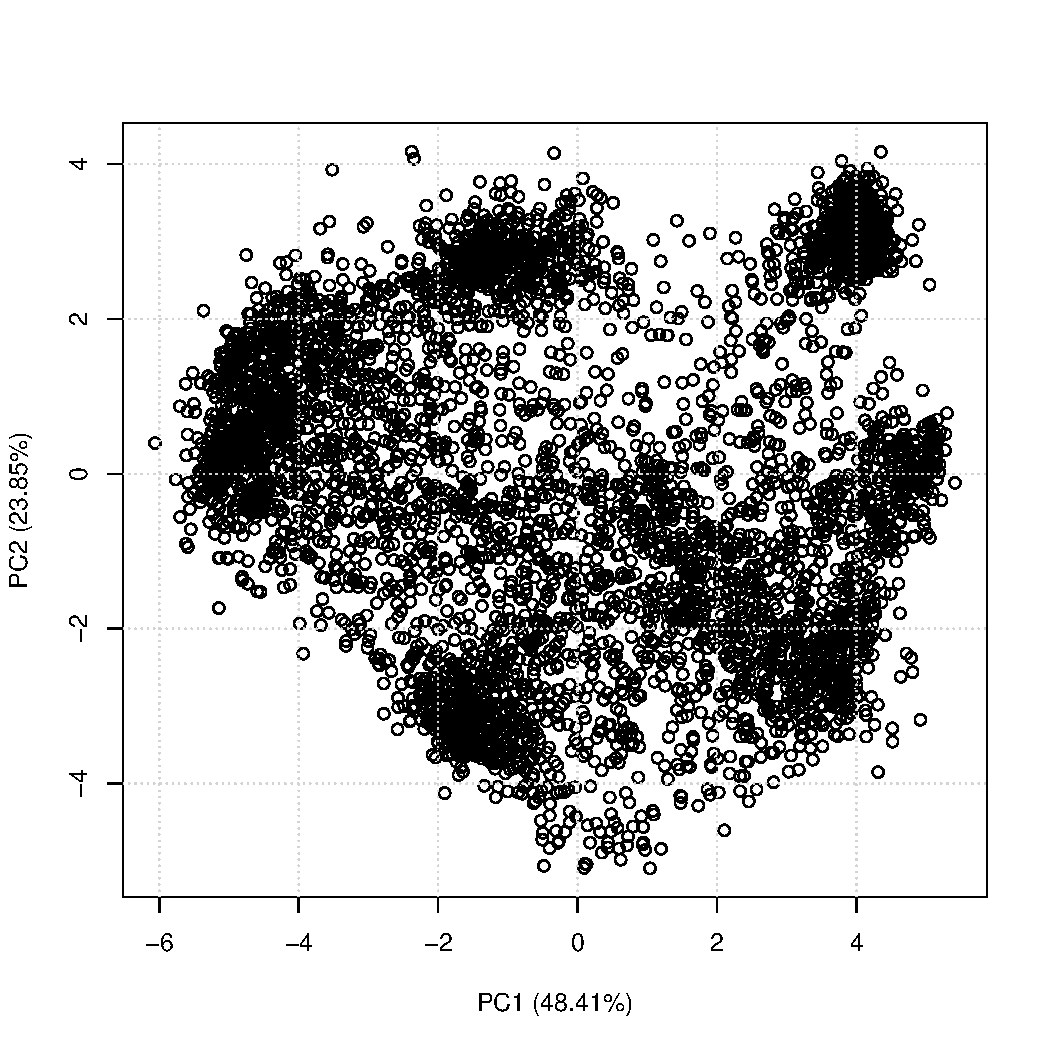
\includegraphics[width = 0.3\textwidth]{./figure/density-1.pdf}
  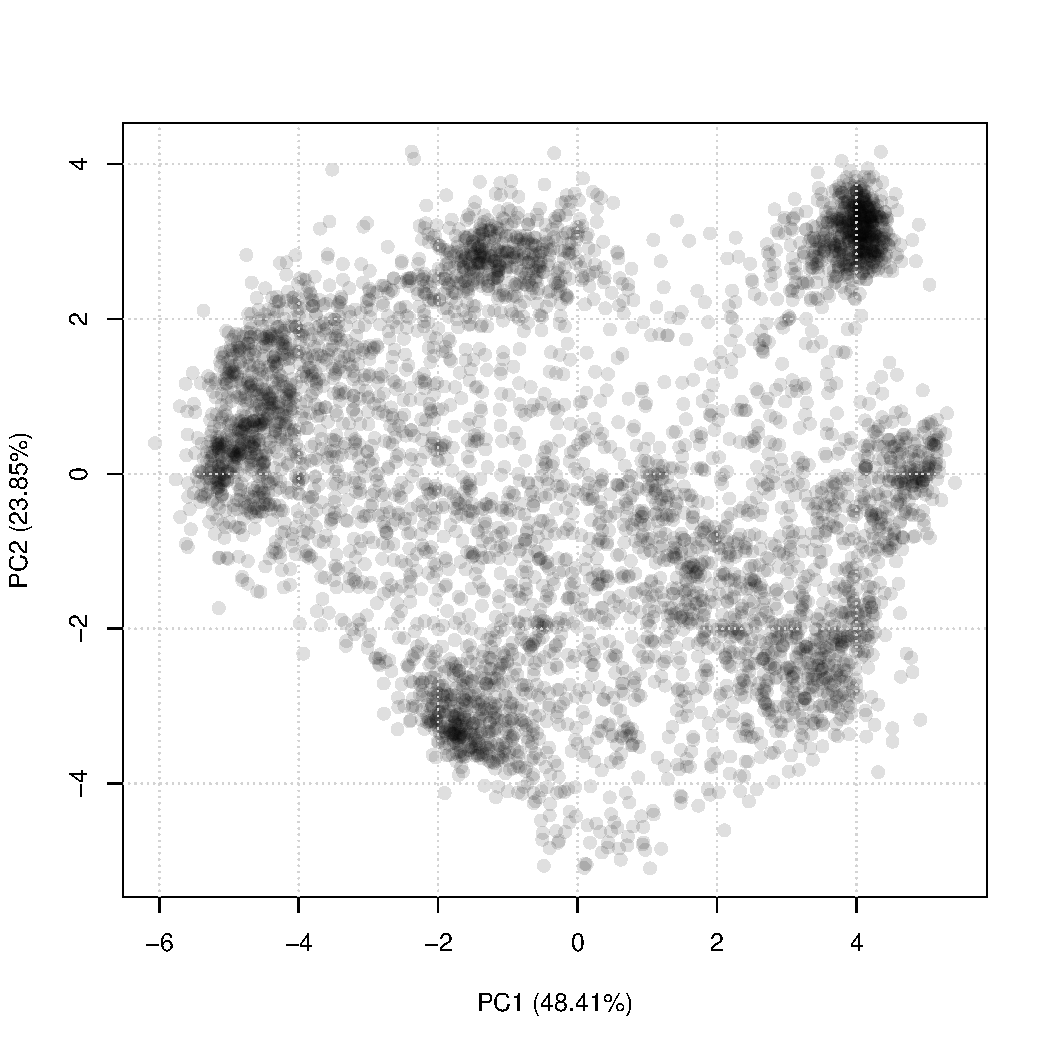
\includegraphics[width = 0.3\textwidth]{./figure/density-2.pdf}
  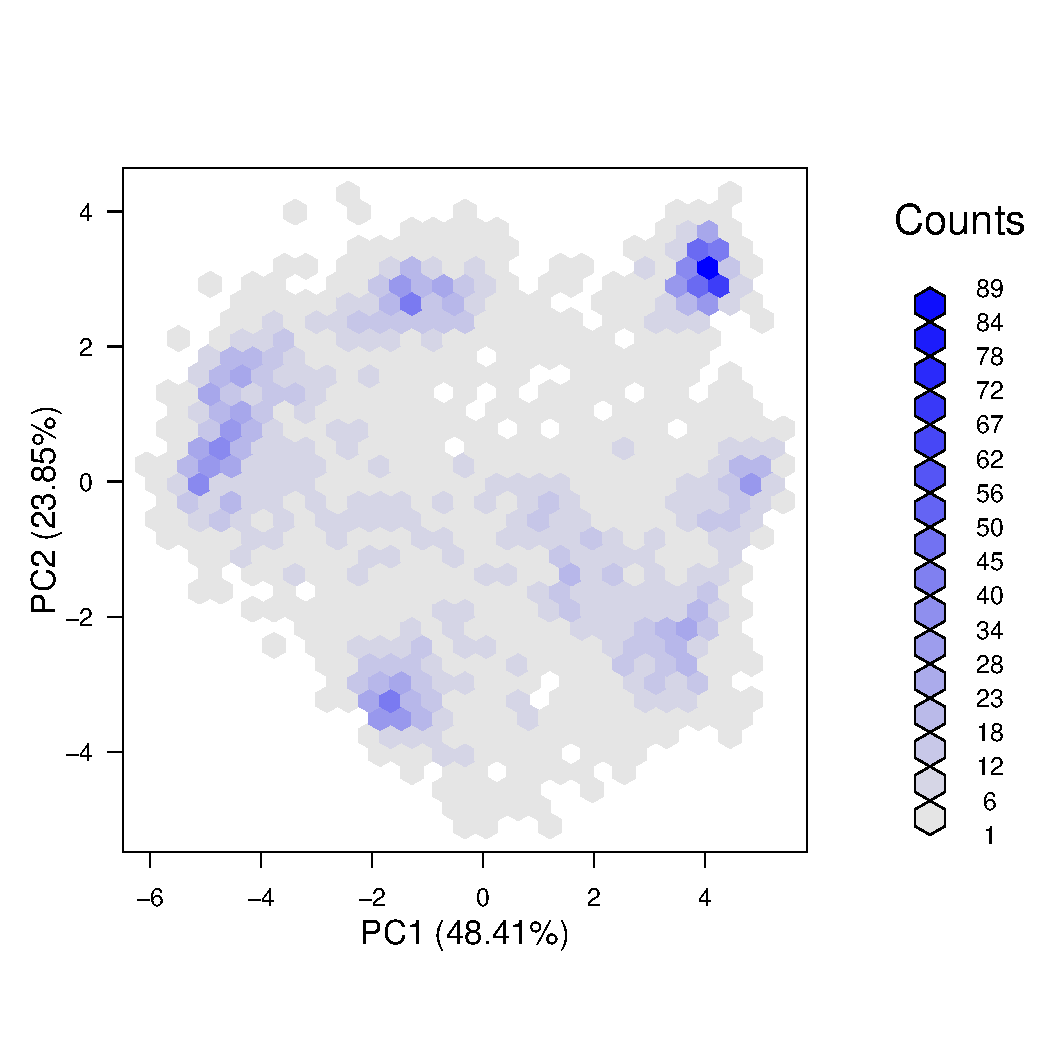
\includegraphics[width = 0.3\textwidth]{./figure/density-3.pdf}
  \caption{Unsupervised visualisation of spatial resolution using the
    \texttt{plot2D} function from the \Biocpkg{pRoloc} package. }
  \label{fig:density}
\end{figure}



In figure~\ref{fig:hexbin1} we compare three datasets to illustrate
different levels of cluster density and separation. We see
areas of high density (many proteins per hexagon)
are highlighted by dark blue, and less
dense areas are white/grey, as indicated by the count key on
the right-hand side of each plot. The figure on the
left is the hyperLOPIT data from \citet{Christoforou:2016} (as on
figure~\ref{fig:density}) that used synchronous precursor selection
(SPS) MS$^3$ on an Orbitrap Fusion. The middle figure represents the
same experiment and same proteins, analysed using conventional MS$^2$,
illustrating the effect of reduced quantitation accuracy. Finally, on
the right, an experiment with considerable less resolution
\citep{Hall:2009}.

\begin{figure}[ht]
  \centering
  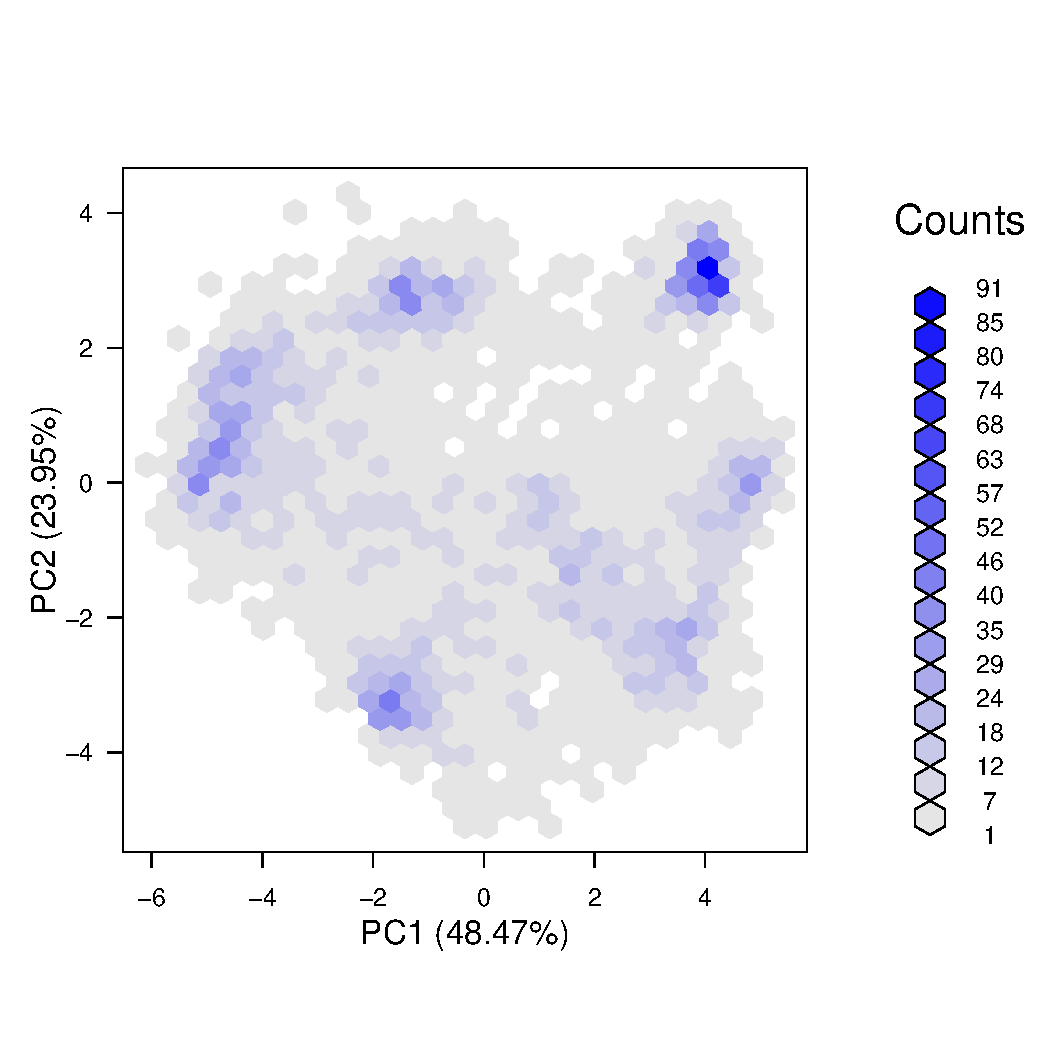
\includegraphics[width = 0.3\textwidth]{./figure/hexbin-1.pdf}
  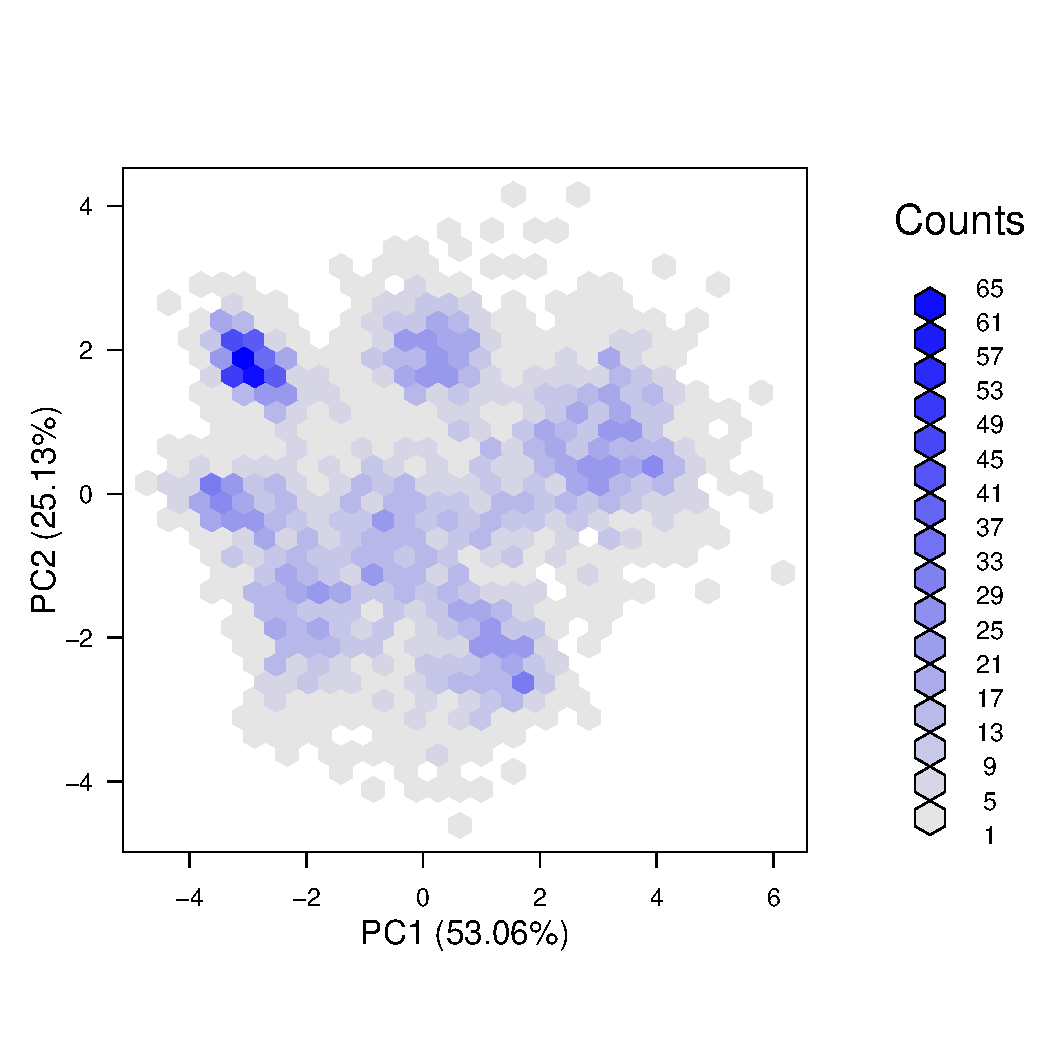
\includegraphics[width = 0.3\textwidth]{./figure/hexbin-2.pdf}
  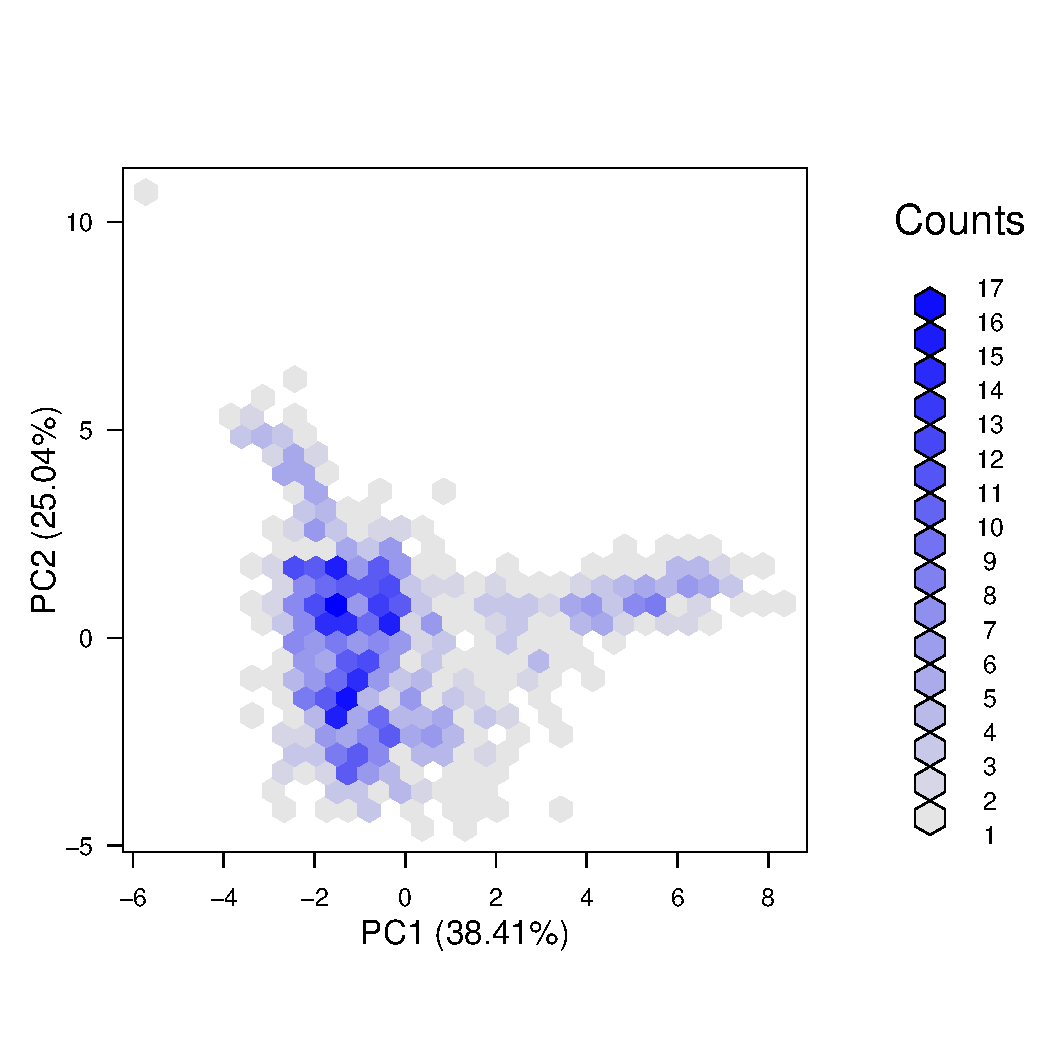
\includegraphics[width = 0.3\textwidth]{./figure/hexbin-3.pdf}
  \caption{Comparing the cluster density and separation of experiments
    with excellent (left), intermediate (centre) and poor (right)
    resolution.}
  \label{fig:hexbin1}
\end{figure}

Considering that the aim of sub-cellular fractionation is to maximise
separation of sub-cellular niches, one would expect sub-cellular
clusters to be separated optimally in a successful spatial proteomics
experiment. In PCA space, this would equate to the location of the
annotated spatial clusters along the periphery of the data points. In
other words, the maximum variability of a successful spatial
proteomics experiments should be reflected by the separation of the
expected/annotated spatial clusters, as illustrated on figure
\ref{fig:pcahl}.

As already mentioned in section~\ref{sec:sub-cell-divers},
sub-cellular niches observed in spatial proteomics are usually
annotated. This annotation comes in the form of marker proteins,
i.e. well-known and trusted residents of a specific niche, for the
species and condition of interest.

\begin{figure}[ht]
  \centering
\begin{knitrout}
\definecolor{shadecolor}{rgb}{0.969, 0.969, 0.969}\color{fgcolor}
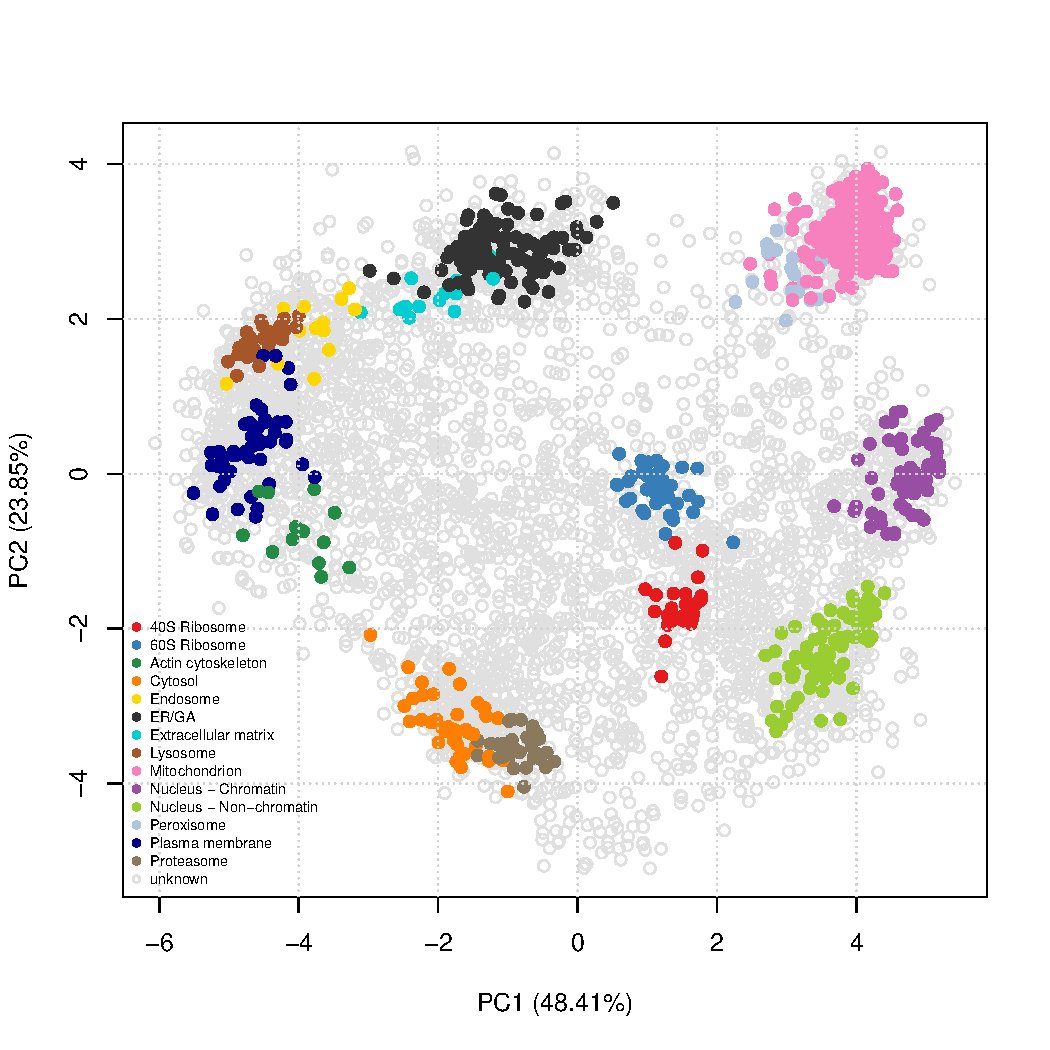
\includegraphics[width=0.75\linewidth]{figure/pcahl-1} 

\end{knitrout}
  \caption{Annotated PCA plot of the \textit{hyperLOPIT2015} dataset.}
  \label{fig:pcahl}
\end{figure}

Another dimensionality reduction method that is worth mentioning here
is linear discriminant analysis (LDA). LDA will project the protein
occupancy profiles in a new set of dimensions using as a criterion the
separation of marker classes by maximising the between class variance
to the within class variance ratio. As opposed to the
\textit{unsupervised} PCA, the \textit{supervised} LDA should not be
used as an experiment quality control, but can be useful to assess if
one or more organelles have been preferentially separated.

\bigskip

It is important to highlight that these representations, while
reflecting a major fraction of the variability in the data, are only a
summary of the total variability. Some sub-cellular niches that
overlap in 2 dimensions can be separated along further components. It
is sometimes useful to visualise data in three dimensions (using for
example the \texttt{plot3D} function in the \Biocpkg{pRoloc} package),
which still, however, only reflect part of the total variability. When
assessing the resolution of some organelles of interest, one should
compare the full protein profiles of the marker proteins
(\Biocpkg{pRoloc}'s \texttt{plotDist} function can be used for this, or
the interactive application \texttt{pRolocVis} in the \Biocpkg{pRolocGUI}
package) or visualise a dendrogram representing the average distance between
cluster profiles (the \texttt{mrkHClust} function from
\Biocpkg{pRoloc} offers this functionality). While detailed
exploration of a dataset using these and other visualisation
approaches is crucial before analysing and interpreting a new spatial
proteomics experiment, a detailed exploration of each of the
29 datasets used in this meta-analysis is out of the
scope of this analysis.

\subsection{Quantifying resolution}\label{sec:qsep}

While visualisation of spatial proteomics data remains essential to
assess the resolution, and hence the success, of a spatial proteomics
experiment, it is useful to be able to objectively quantify the
resolution and directly compare different experiments. Here, we
present a new infrastructure, termed \texttt{QSep}, available in the
\Biocpkg{pRoloc} package \citet{Gatto:2014a}, to quantify the
separation of clusters in spatial proteomics experiments. It relies on
the comparison of the average euclidean distance \textit{within} and
\textit{between} sub-cellular clusters. As illustrated on the heatmaps
in figure~\ref{fig:qsep0} for the \textit{hyperLOPIT2015} data, these
distances always refer to one reference marker cluster.

The raw distance matrix (figure~\ref{fig:qsep0}, top-left) is
symmetrical (i.e. the distance between cluster 1 and 2 is the same as
between cluster 2 and 1). Within distances are generally the smallest
ones, except when two clusters overlap, as the lysosome and endosome
in our example. To enable the comparison of these distances within and
between experiments (see section~\ref{sec:compara} for the latter), we
further divide each distance by the reference within cluster average
distance (figure~\ref{fig:qsep0}, top-right). This thus informs us as
how much the average distance between cluster 1 and 2 is greater than
the average distance within cluster 1 (i.e. the tightness of that
cluster). At this stage, the distance matrix is no longer
symmetrical. To facilitate the comparison of distances between
organelles, the distance distributions can also be visualised as
boxplots (figure~\ref{fig:qsep0}, bottom).









\begin{figure}[!ht]
  \centering
  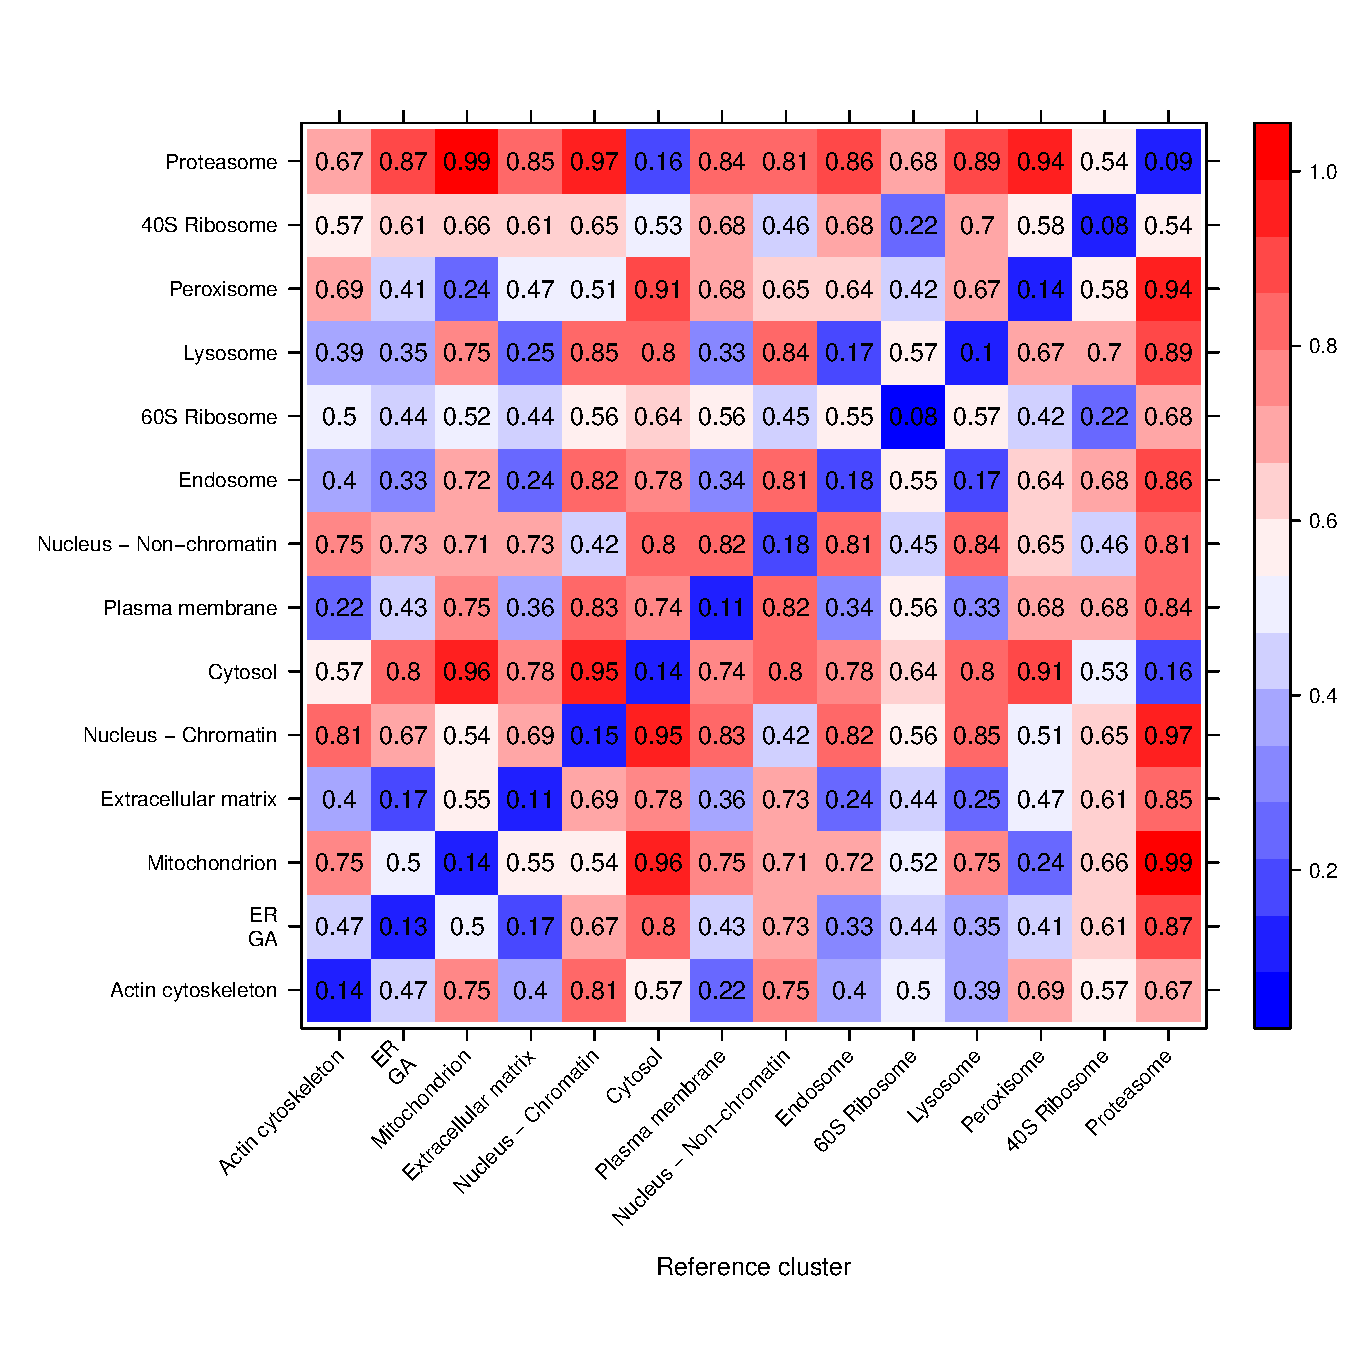
\includegraphics[width = 0.45\textwidth]{./figure/qsep0lv-1.pdf}
  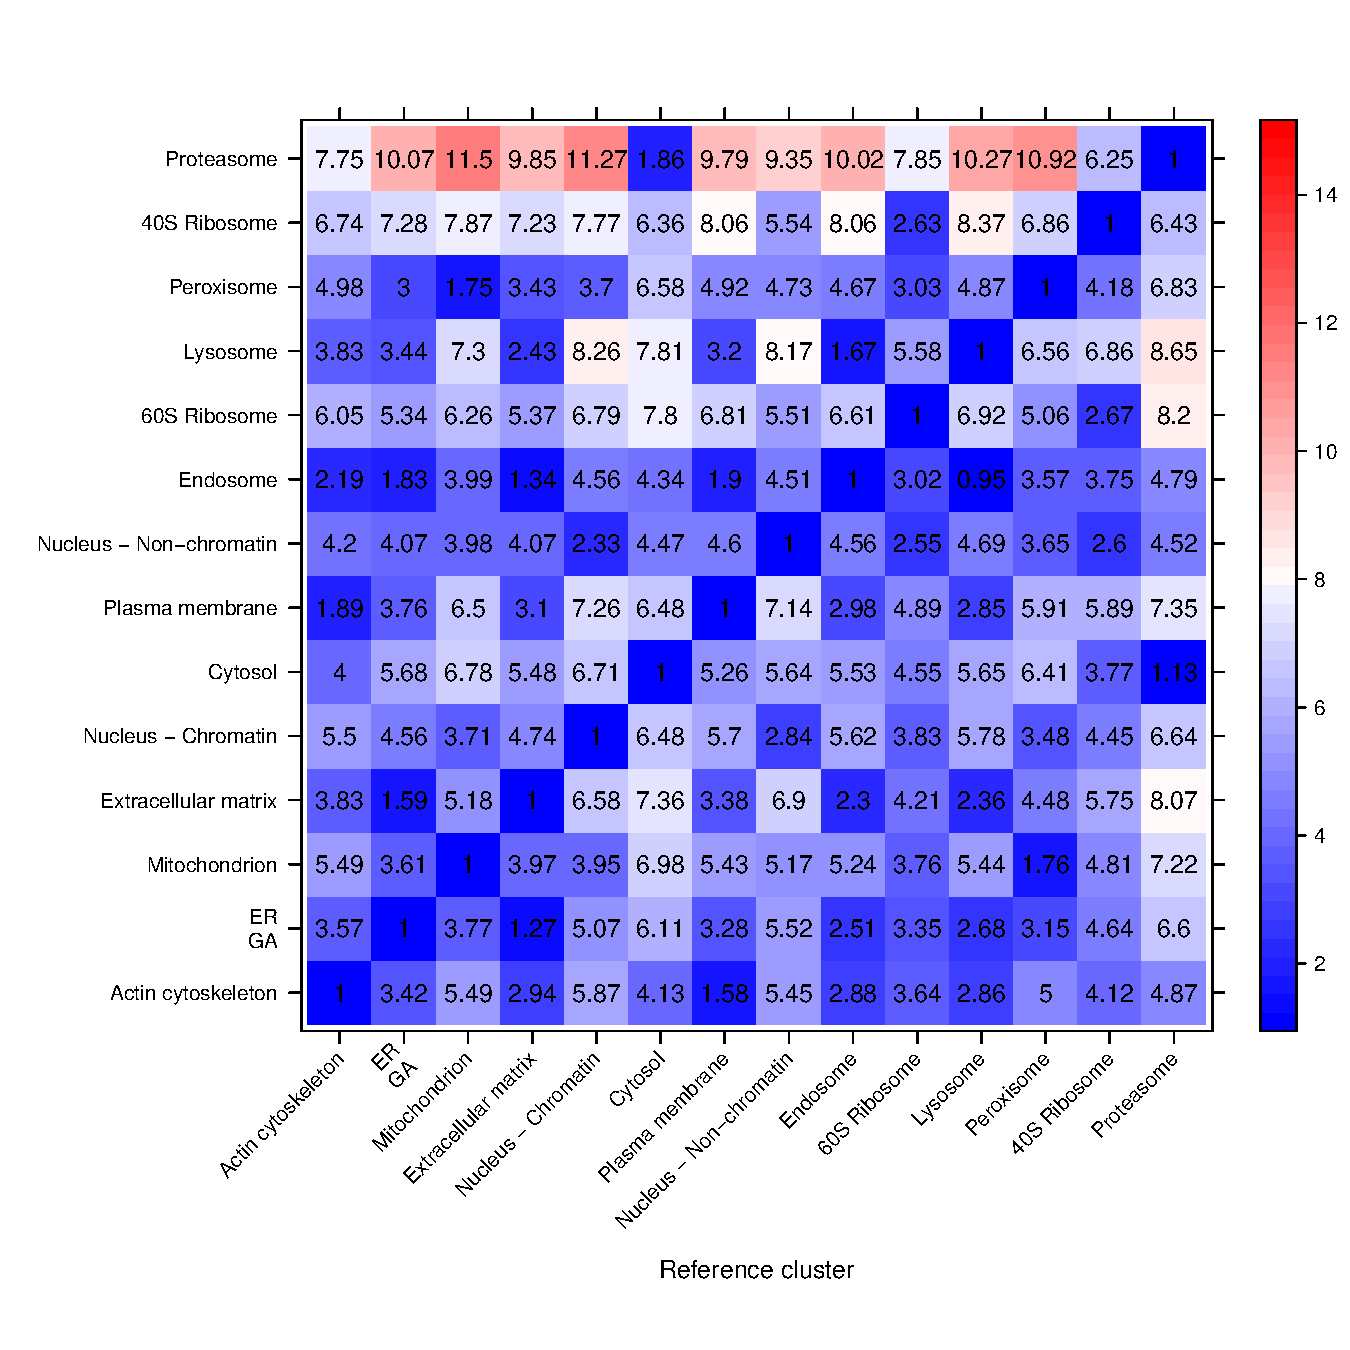
\includegraphics[width = 0.45\textwidth]{./figure/qsep0lv-2.pdf}
  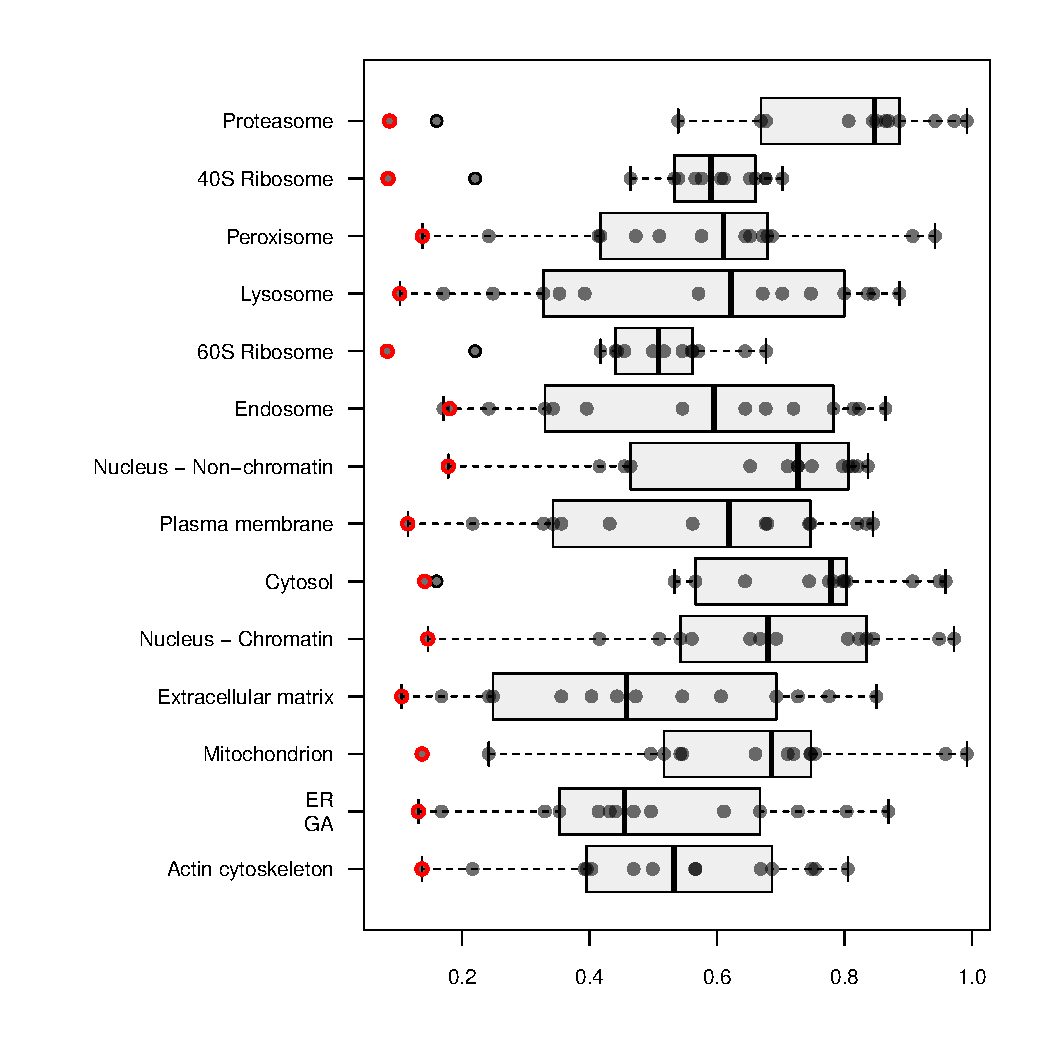
\includegraphics[width = 0.45\textwidth]{./figure/qsep0bx-1.pdf}
  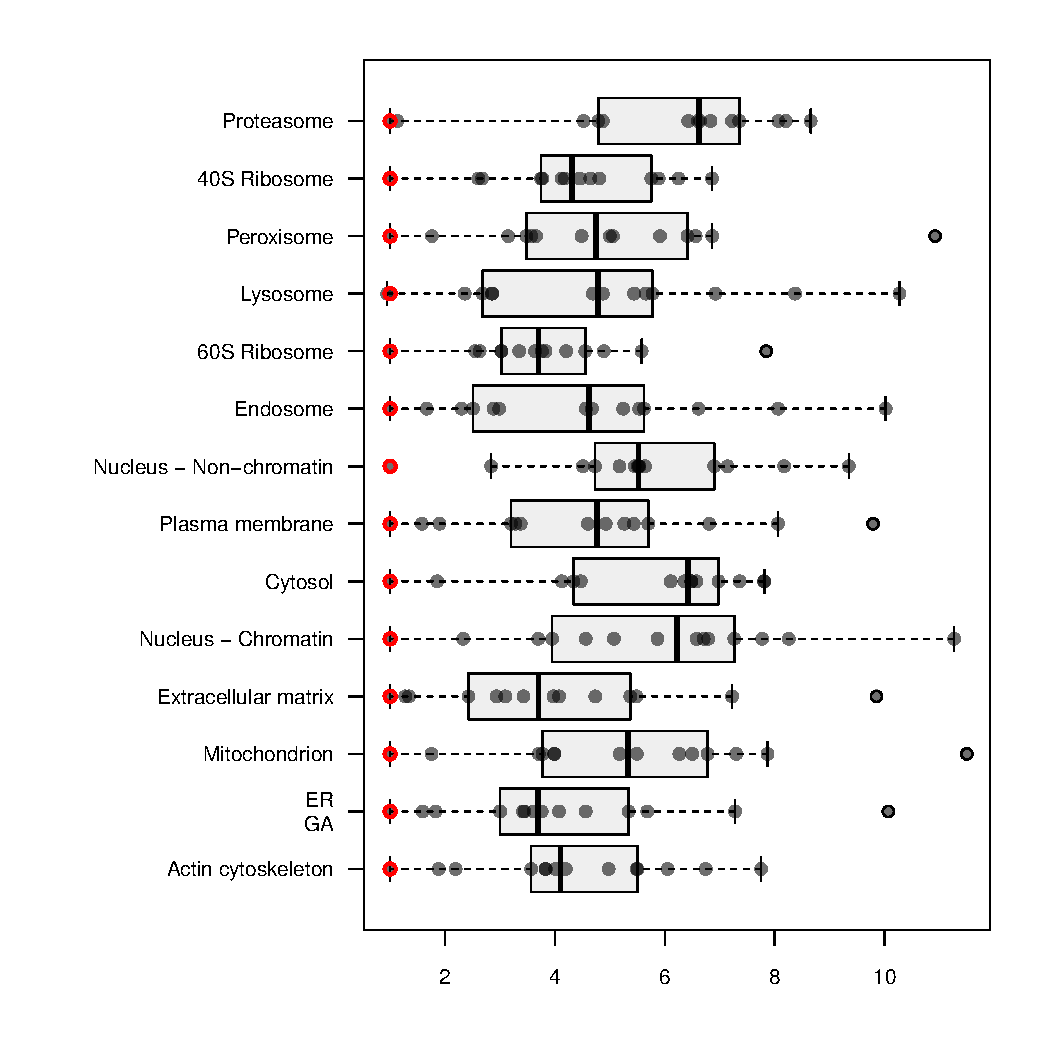
\includegraphics[width = 0.45\textwidth]{./figure/qsep0bx-2.pdf}
  \caption{Quantifying resolution of the \textit{hyperLOPIT2015} data
    \citet{Christoforou:2016}. The heatmaps at the top illustrate the
    raw (left) and average normalised (right) within (along the
    diagonal) and between euclidean cluster distances. The boxplots at
    the bottom summarise these same values (raw on the left,
    normalised on the right) to enable easier comparison between
    clusters, where the within distances are highlighted in red. }
  \label{fig:qsep0}
\end{figure}


The rational behind these measures is as follows. Intuitively, we
assess resolution by contrasting the separation between clusters
(formalised by the average distance between two clusters) and the
tightness of single clusters (formalised by the average within cluster
distance). Ideal sub-cellular fractionation would yield tight and
distant clusters, represented by a large normalised between cluster
distances on figure \ref{fig:qsep0}.

\clearpage

\subsection{Application of the assessment criteria}\label{sec:applic}



To further demonstrate the interpretation of these resolution metrics,
we directly compare the two recent global cell maps from
\cite{Christoforou:2016} (dataset \textit{hyperLOPIT2015}) and
\cite{Itzhak:2016} (dataset \textit{itzhak2016stcSILAC}). Both feature
high protein coverage (7114 and 5265 proteins
respectively) and good sub-cellular diversity (14 and
12 annotated clusters respectively). The former contains
duplicated experiments, each made of 10 fractions and the latter
contains 6 replicates with 5 fractions each. Figure~\ref{fig:pcacmp}
shows the PCA plots applying transparency to identify the underlying
structure in the quantitative data and the annotated versions using
the markers provided by the respective authors.

\begin{figure}[!h]
  \centering
\begin{knitrout}
\definecolor{shadecolor}{rgb}{0.969, 0.969, 0.969}\color{fgcolor}
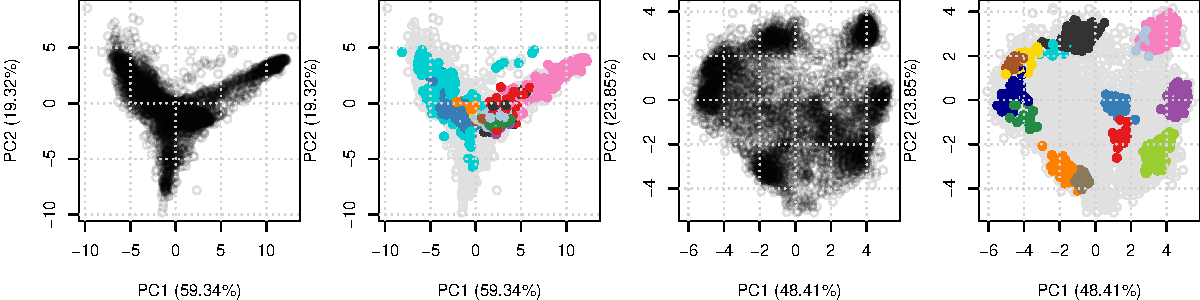
\includegraphics[width=\maxwidth]{figure/pcacmp-1} 

\end{knitrout}
\caption{PCA plots for \textit{itzhak2016stcSILAC} (left) and
  \textit{hyperLOPIT2015} (right). Here, we display PC 1 and 2 for
  both datasets for comparability. The original authors displayed PC 1
  and 3 for the \textit{itzhak2016stcSILAC} data (see
  figures~\ref{fig:denspca} and~\ref{fig:pca} below).}
  \label{fig:pcacmp}
\end{figure}


Figure~\ref{fig:qsepcmp} illustrates the normalised distance heatmaps
and boxplots for the two datasets (\textit{itzhak2016stcSILAC} at the
top and \textit{hyperLOPIT2015} at the bottom). The two heatmaps
display strikingly different colour patterns. The top heatmap shows a
majority of small normalised distances (blue cells) and with only a
limited number of large distances (red cells), along the mitochondrial
reference cluster. Conversely, the bottom heatmap displays a majority
of average (white cells) and large distances (red cells) across all
sub-cellular clusters. The boxplots allow a more direct comparison of the
distances across the two datasets. On the top boxplot, we detect
relatively short distances for most clusters, with most large
distances stemming from the mitochondria, leading to a median distance
of 2.48. The distributions on the bottom boxplot
show larger distances, equally spread among all clusters, with an
median distance of 4.91.

\begin{figure}[h]
  \centering
  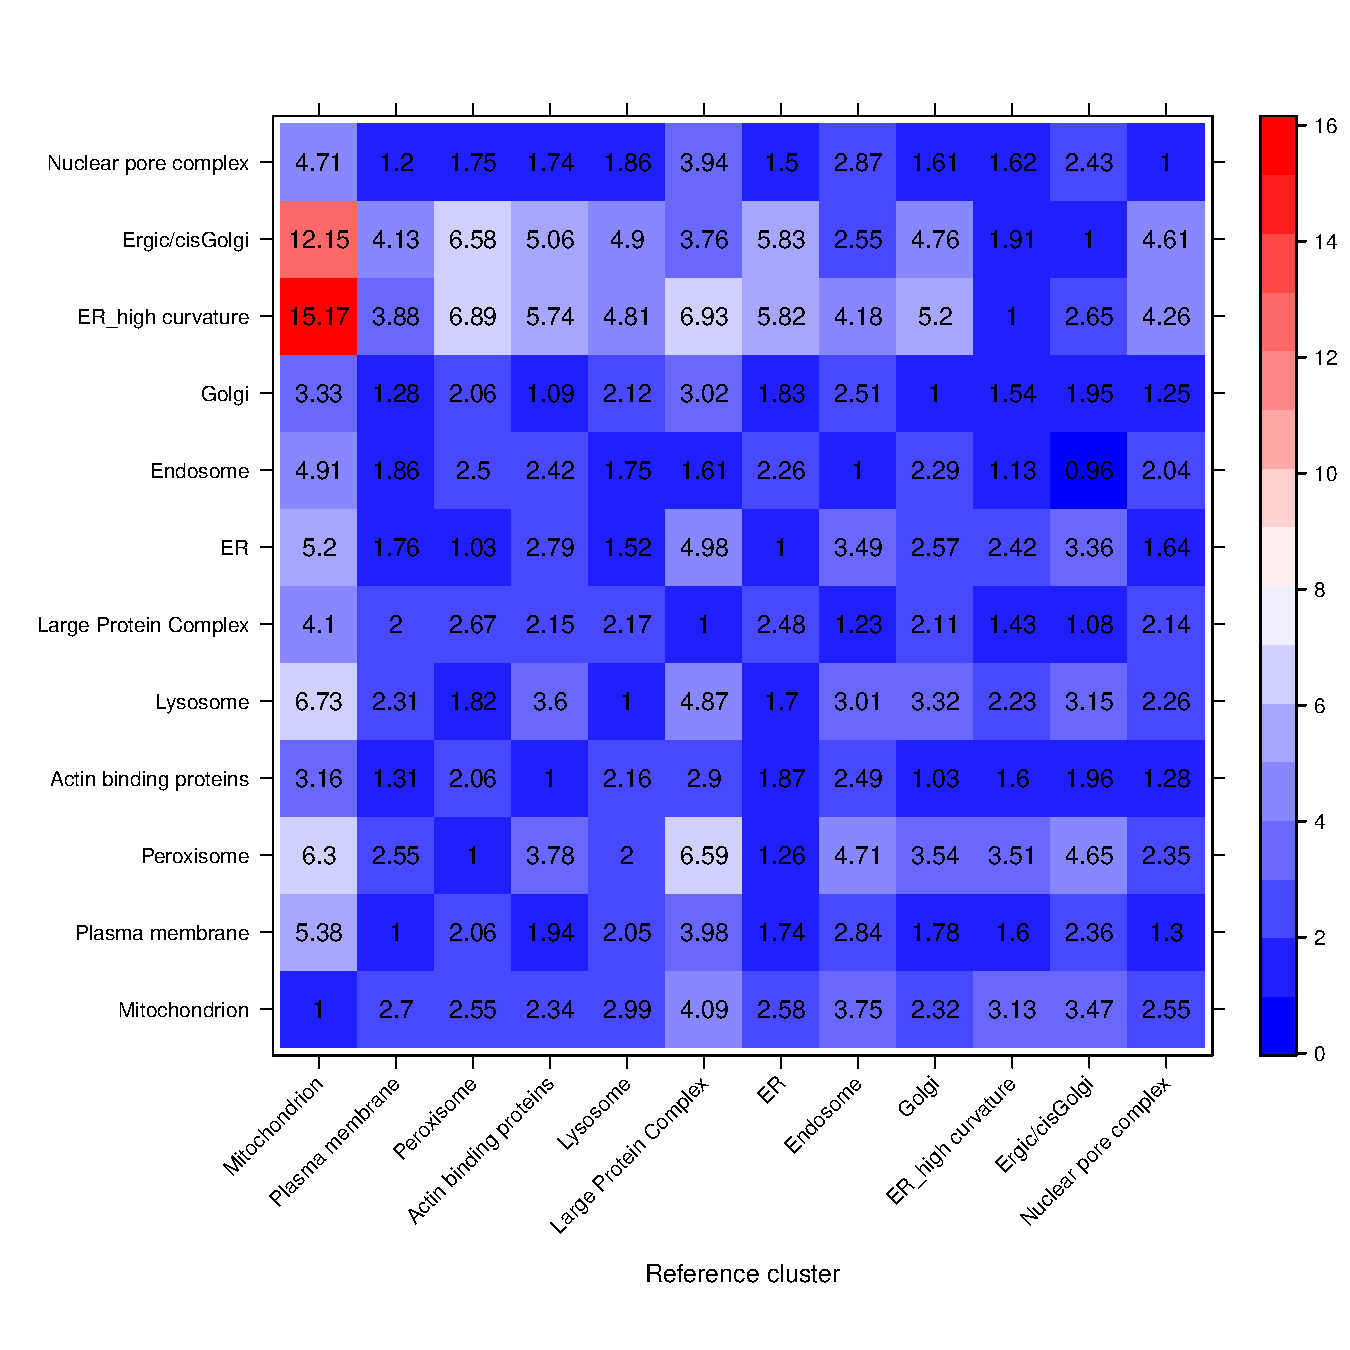
\includegraphics[width = 0.45\textwidth]{./figure/qsep0lv-3.pdf}
  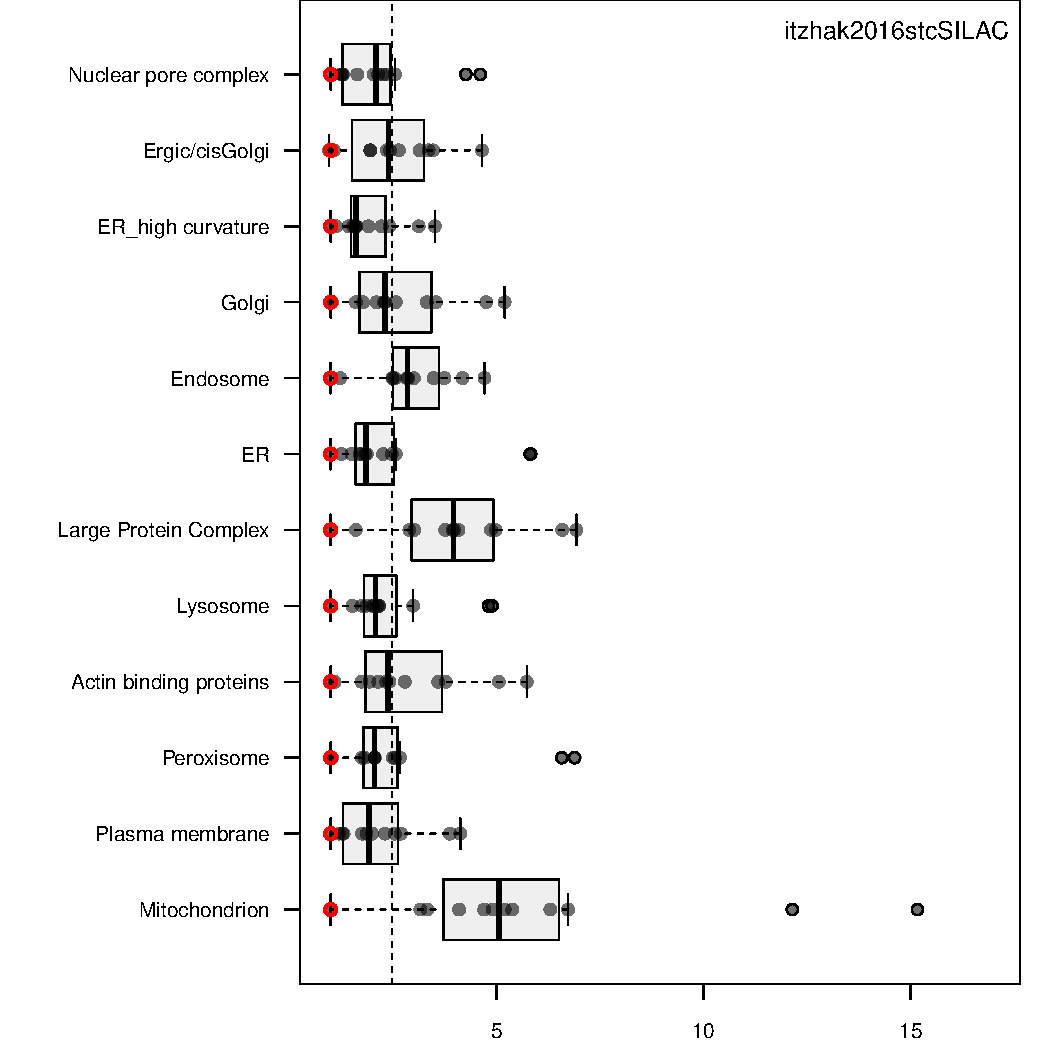
\includegraphics[width = 0.45\textwidth]{./figure/qsepcmp-2.pdf}
  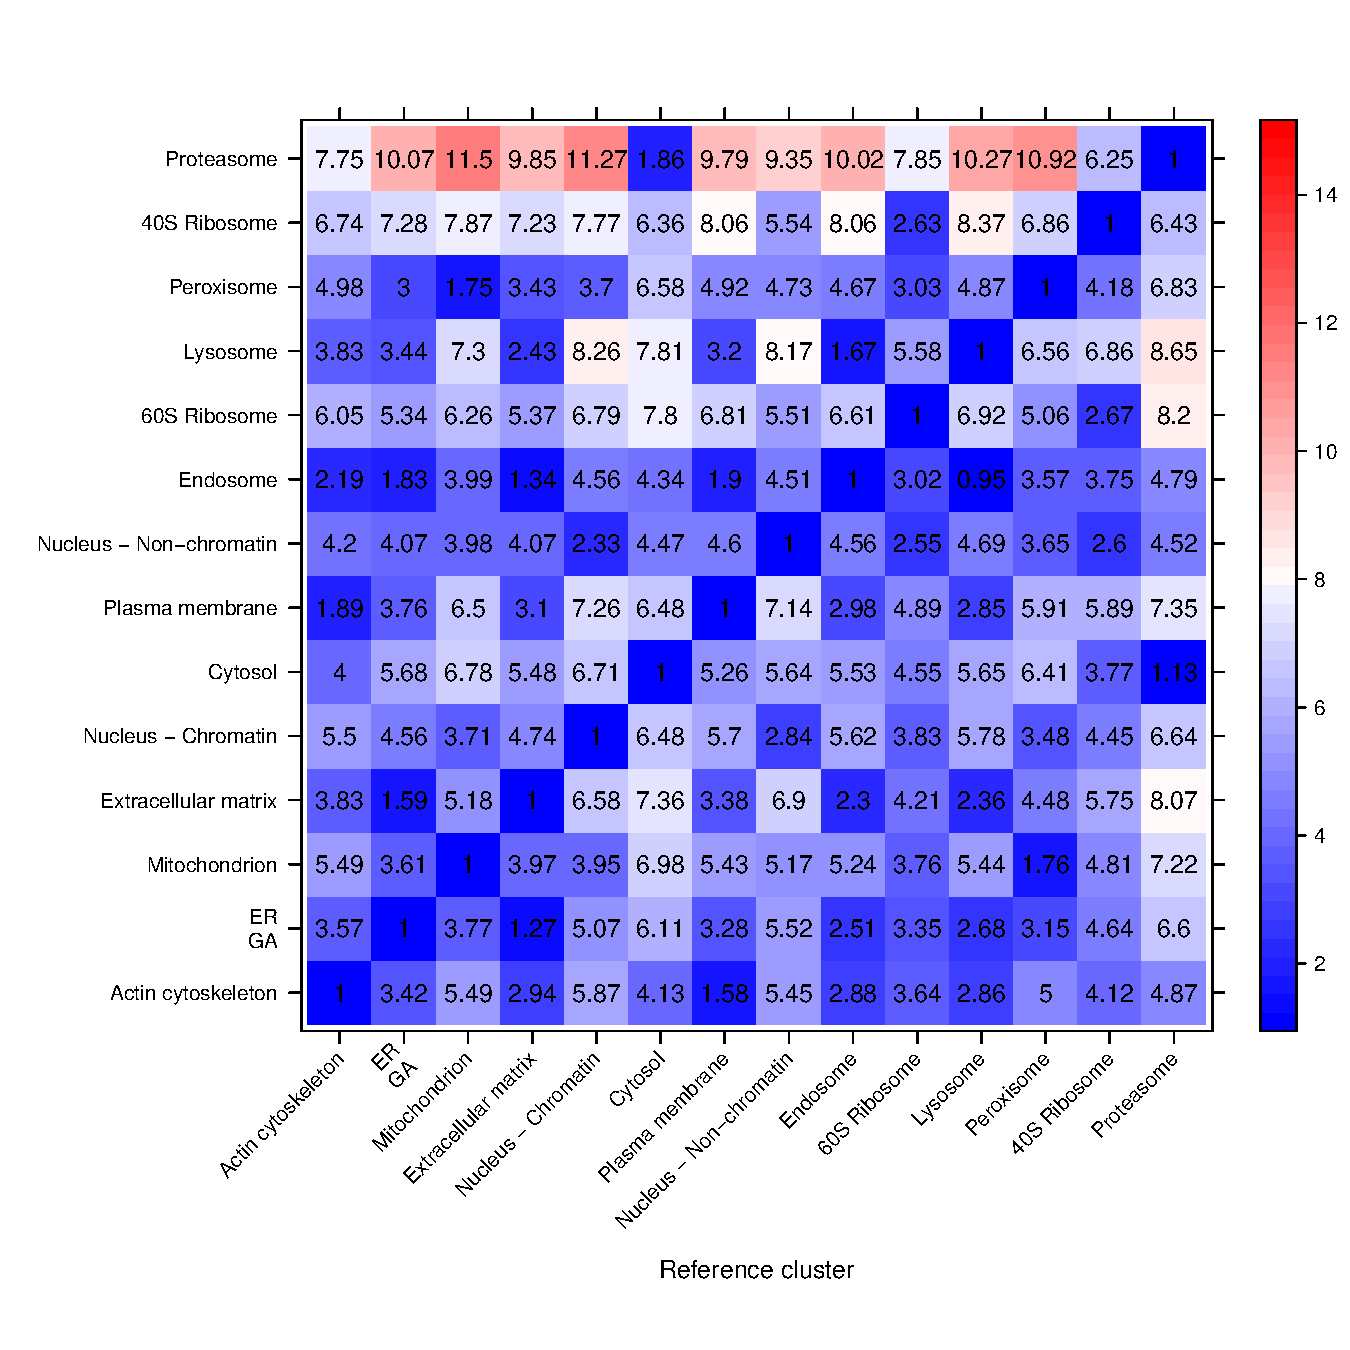
\includegraphics[width = 0.45\textwidth]{./figure/qsep0lv-2.pdf}
  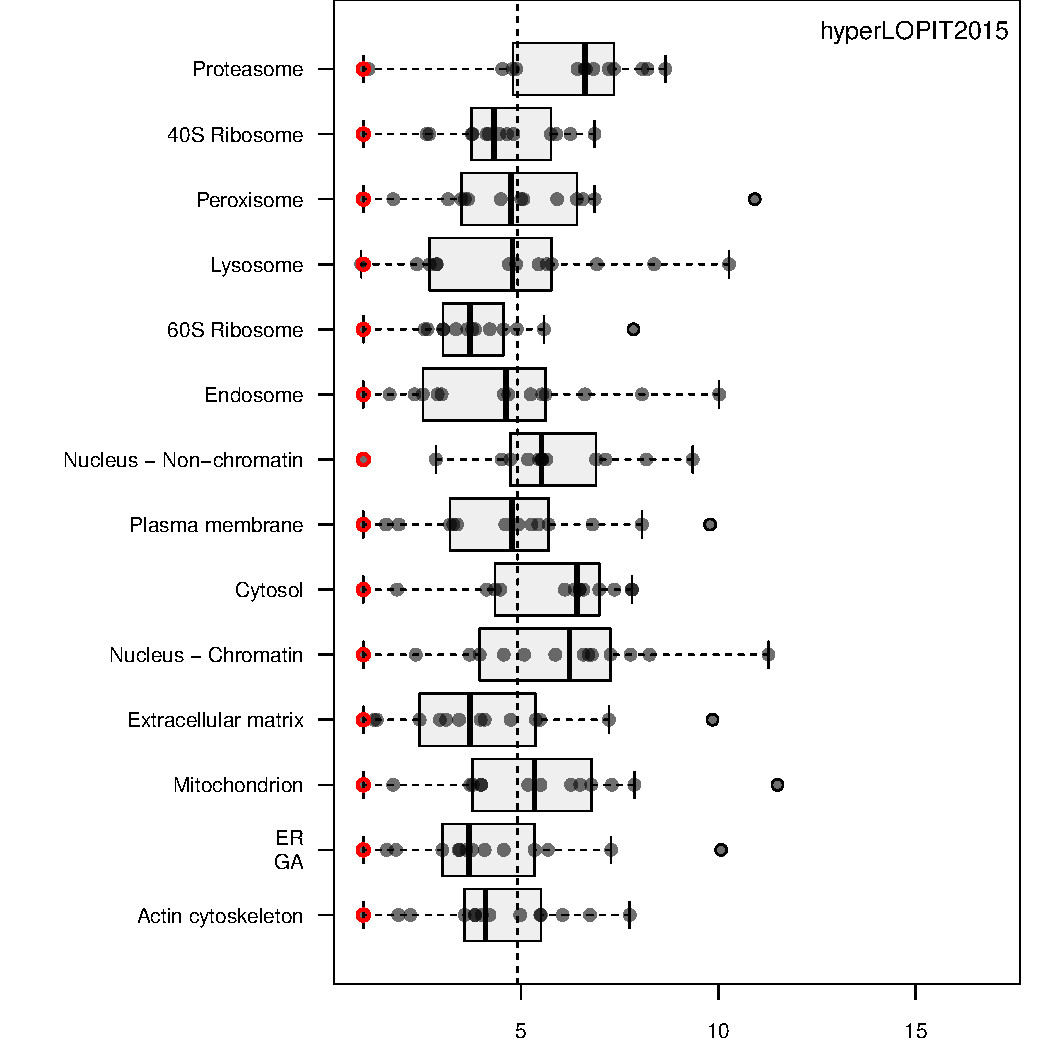
\includegraphics[width = 0.45\textwidth]{./figure/qsepcmp-1.pdf}
  \caption{Contrasting quantitative separation assessment between the
    \textit{itzhak2016stcSILAC} \citep{Itzhak:2016} (top) and
    \textit{hyperLOPIT2015} \citep{Christoforou:2016} (bottom)
    datasets. The dashed vertical lines on the boxplots represent the
    overall media between cluster distance, 2.48 and
    4.91 for \textit{itzhak2016stcSILAC} and
    \textit{hyperLOPIT2015} respectively. }
  \label{fig:qsepcmp}
\end{figure}

\clearpage

\section{Comparative study}\label{sec:compara}

We next apply the quantitative assessment of spatial resolution
described in section~\ref{sec:qsep} to compare the 29
experiments presented in section~\ref{sec:pdata}. On
figure~\ref{fig:qsep}, we show, for each dataset, a boxplot
illustrating the distribution of the global average normalised
distances for all spatial clusters. The datasets have been ordered
using the experiment-wide median between distance. It is important to
always refer back to the original data when considering
summarising metrics like these, to put the resolution into context;
the density and annotated PCA plots discussed in section~\ref{sec:vis}
are provided in figures~\ref{fig:denspca} and~\ref{fig:pca} and the
quantitative assessment boxplots and heatmaps are shown in
figures~\ref{fig:allqseps} and~\ref{fig:allhmaps}.



\begin{figure}[ht]
  \centering
\begin{knitrout}
\definecolor{shadecolor}{rgb}{0.969, 0.969, 0.969}\color{fgcolor}
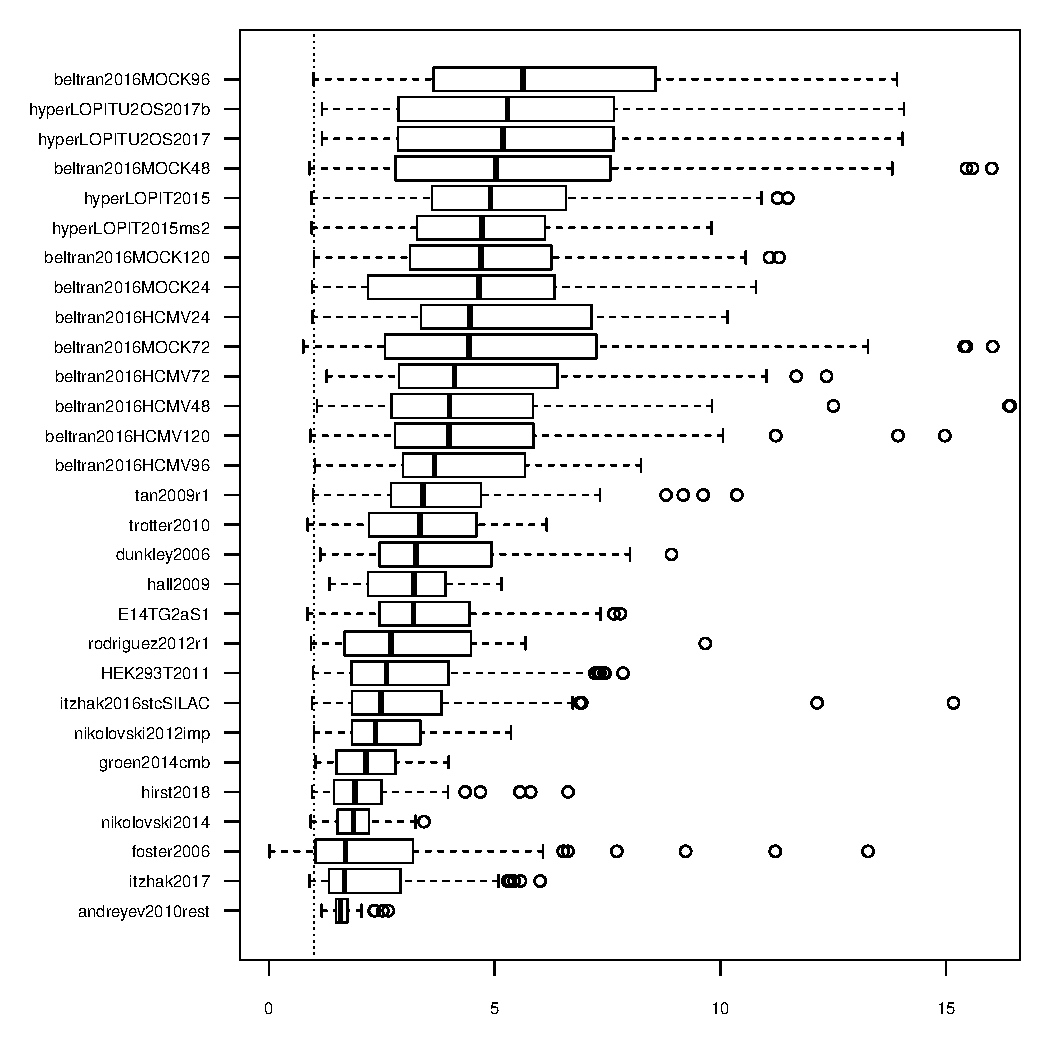
\includegraphics[width=0.65\linewidth]{figure/figqsep-1} 

\end{knitrout}
\caption{Quantitative separation assessment using experiment-wide
  normalised distances between cluster distances. The vertical line
  represents the normalised intra-cluster distance of 1.}
  \label{fig:qsep}
\end{figure}


The hyperLOPIT experiments \textit{hyperLOPIT2015} and
\textit{hyperLOPIT2015ms2} \citep{Christoforou:2016} using SPS MS$^3$
and conventional MS$^2$ show the best global, experiment-wide
resolution. As documented by the authors and illustrated in
section~\ref{sec:vis}, the increased quantitation accuracy of the
former result in better sub-cellular resolution.

The next set of experiment are \textit{tan2009r1},
\textit{trotter2010}, \textit{dunkley2006}, \textit{hall2009} and
\textit{E14TG2aS1}. It is important to highlight that most of datasets
(as well as \textit{HEK293T2011}, discussed later) have either been
directly re-analysed using a semi-supervised novelty detection
algorithm \textit{phenoDisco} \citep{Breckels:2013} (the only
exception here being \textit{hall2009}), or, in the case of
\textit{trotter2010}, have been annotated using markers based on the
\textit{phenoDisco} re-analysis. The novelty detection algorithm,
\textit{phenoDisco}, searches for new clusters of unlabelled proteins,
using the marker proteins to guide the clustering of unlabelled
features. These new clusters, termed \textit{phenotypes}, are then
validated by the user for coherence with known sub-cellular niches.
This re-analysis has proven successful \citep{Breckels:2013} and has
identified previously undetected sub-cellular niches that form tight
and well-resolved clusters (see for example ribosomial and trans-Golgi
network (TGN) in \textit{dunkley2006}, or proteasome and nucleus in
\textit{tan2009r1} to cite only a few), which in turn favour good
resolution scores. The \textit{hall2009} dataset is relatively poorly
annotated (only 5 sub-cellular clusters, which is the lowest in all
test datasets). As long as these few clusters are well separated, poor
annotation will not negatively influence the resolution scoring,
emphasising the importance of data visualisation
(section~\ref{sec:vis}).



The next set of experiments that show comparable resolution profiles
are \textit{HEK293T2011}, \textit{itzhak2016stcSILAC} and
\textit{nikolovski2012imp}. Note that the quantitative separation
measurement is robust to questionable marker annotation. For example,
the \textit{Large Protein Complex} class defined by the original
authors in the \textit{itzhak2016stcSILAC} data could be dropped as it
loosely defines many niches and thus lacks resolution. This omission only
marginally influences the overall assessment metrics as only the
distances to/from that class are affected (i.e. 23
out of 144 distances) and as such it would not change its
rank among the test datasets.

As mentioned earlier, the \textit{groen2014cmb} and
\textit{nikolovski2014} are targeted experiments, focusing on the
trans-Golgi-network and Golgi niches respectively. Such experiments do
not aim for the best global resolution, which is reflected by relatively
low resolution.

The \textit{foster2006} experiment displays relatively poor
separation. This might be due to the relatively high number of missing
values (42.4 \%). Finally, the \textit{andreyev2010rest} dataset suffers from
very broad sub-cellular clusters (compared to separation between
clusters).

%% HERE

\bigskip

The PCA plots and QSep heatmaps for all datasets are provided in the
appendix, section \ref{sec:figs}.










\section{Assessing the resolution metric}\label{sec:qsepassess}

In this section, we assess the resolution metric, and how the
annotation of the spatial proteomics data influences the metric
itself.



We find that the number of classes does not have any effect the resolution
assessment scoring. Indeed, dropping any class will result in a
sub-sample of normalised inter-cluster distances, with random
variations around the overall median inter-cluster distance. On
figure~\ref{fig:simn}, we show the distribution of the resolution
metrics when removing all possibly combinations of 1 to 3 sub-cellular
classes for the \textit{E14TG2aS1} dataset, that displays an average
overall resolution, and \textit{hyperLOPIT2015}, that has a highest
resolution. In both cases, we see that the number of removed classes
does not influence the overall score distributions. When modelling the
linear relation between the median scores and the number of removed
classes, the slopes are 0.036 and
0.01 respectively.

\begin{figure}[h]
  \centering
  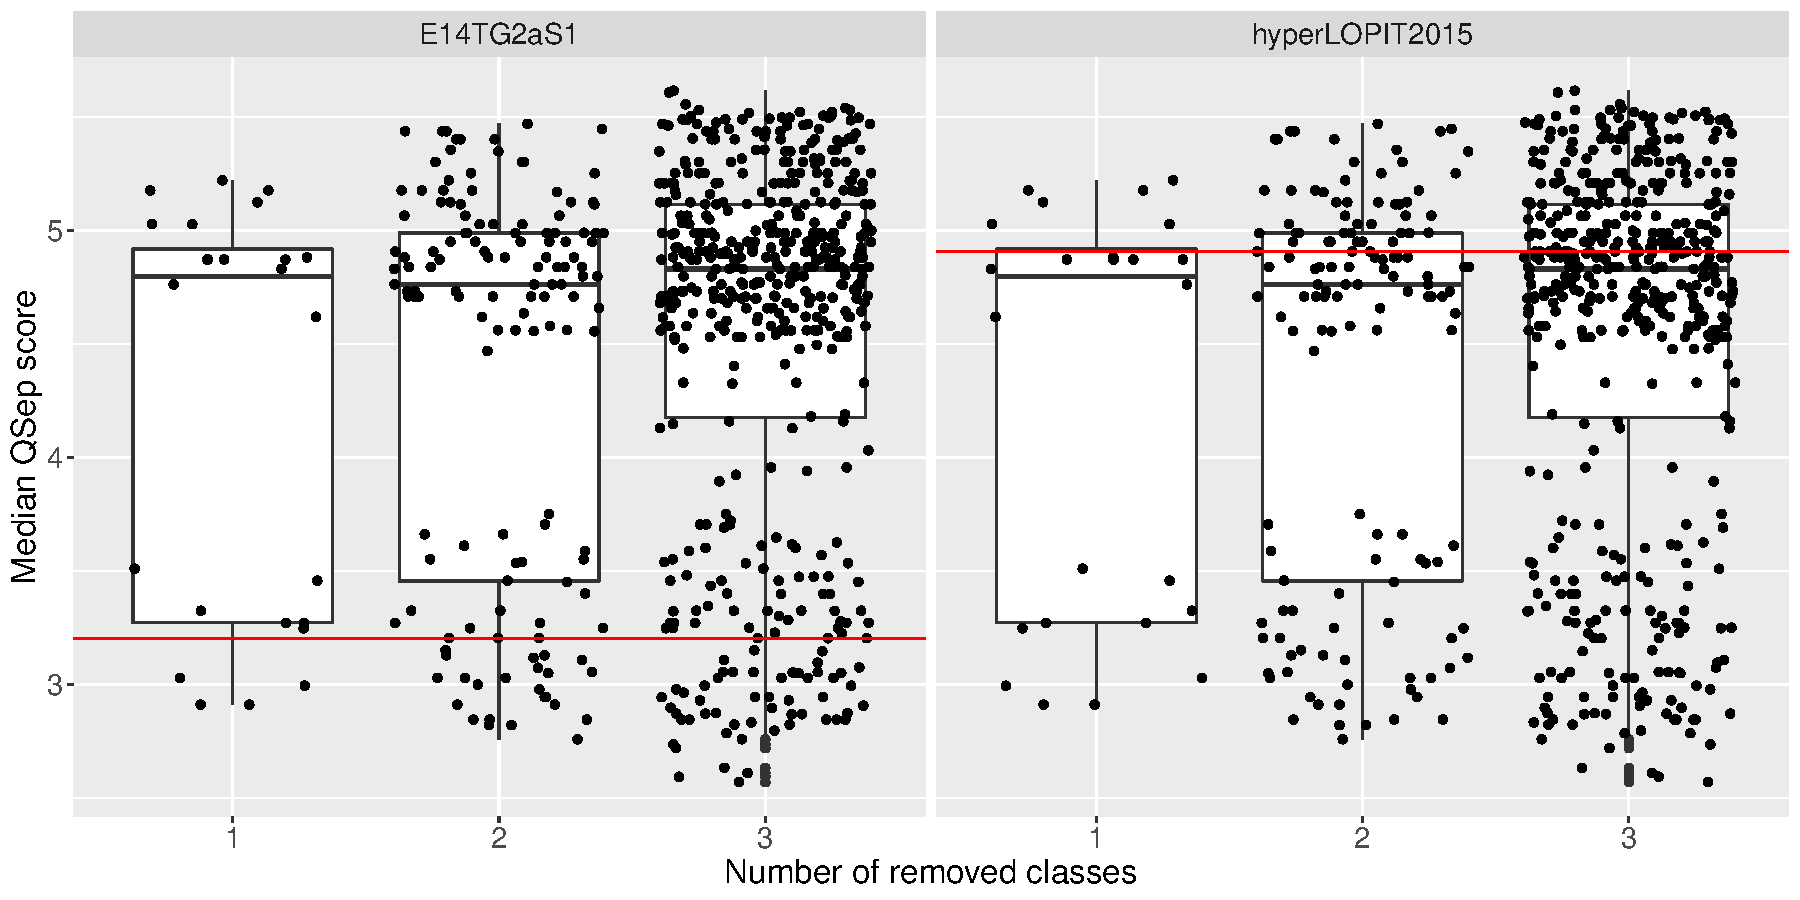
\includegraphics[width = .7\textwidth]{simn.pdf}
  \caption{Effect of removing sub-cellular clusters on the resolution
    metric for the \textit{E14TG2aD1} (left) and
    \textit{hyperLOPIT2015} experiments (right). Each dot represents a
    median resolution score for the experimental setting (i.e missing
    $n$ classes). The horizontal lines represents the median resolution
    metrics for the complete dataset. Note the overall higher median
    assessment scores for the better \textit{hyperLOPIT2015}
    experiment }
  \label{fig:simn}
\end{figure}

The definition of marker proteins has of course an effect on the
assessment metric. Tighter clusters will result in smaller intra-class
distances and, as a result, in larger normalised inter-class
distances. To assess the effect of marker definition, we transferred
the marker annotation between the \textit{hyperLOPIT2015} and
\textit{itzhak2016stcSILAC} datasets (see PCA plots on
figure~\ref{fig:mrkswtch}, left) and calculated the quantitative
resolution metrics (see boxplots on figure~\ref{fig:mrkswtch},
right).

\begin{figure}[h]
  \centering
  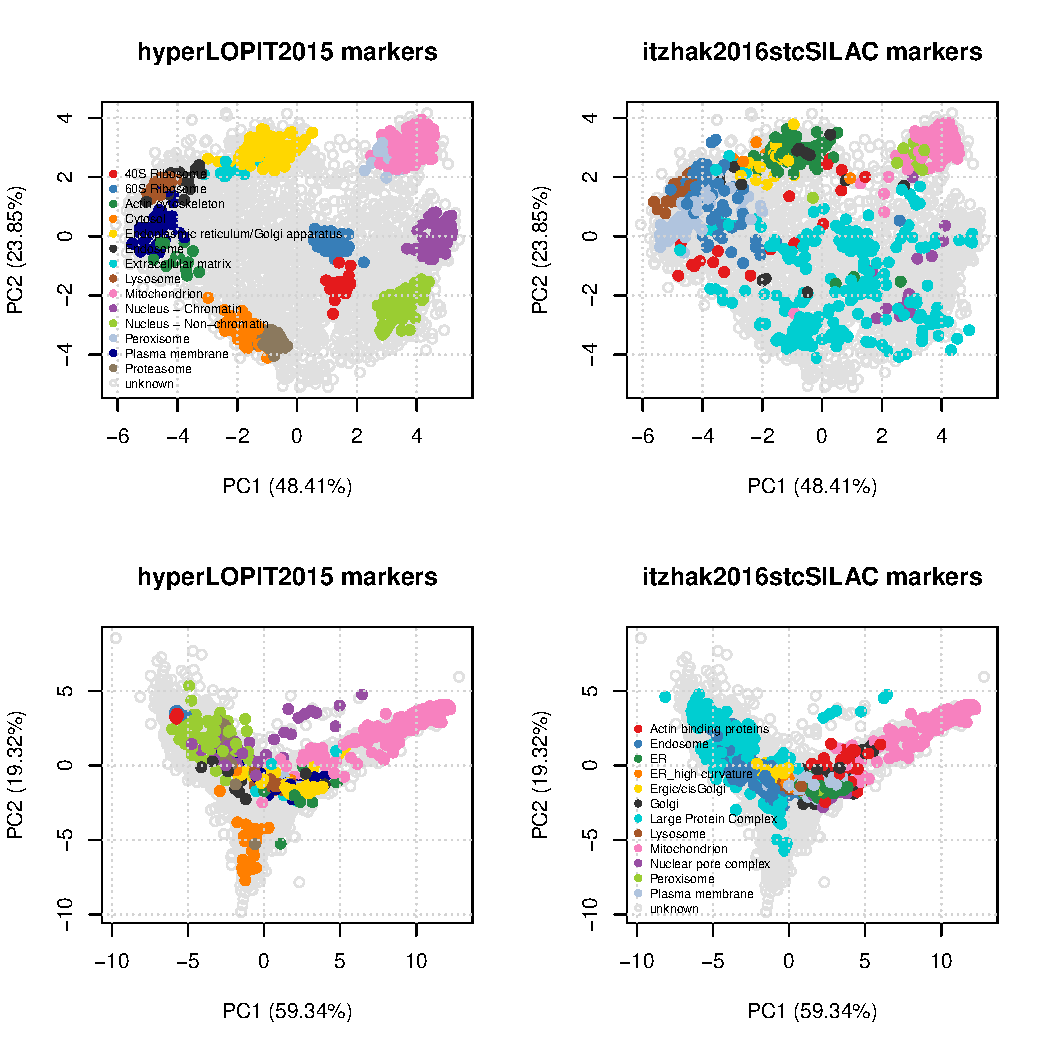
\includegraphics[width = 0.54\textwidth]{mrkswtch-pca.pdf}
  \raisebox{.1\height}{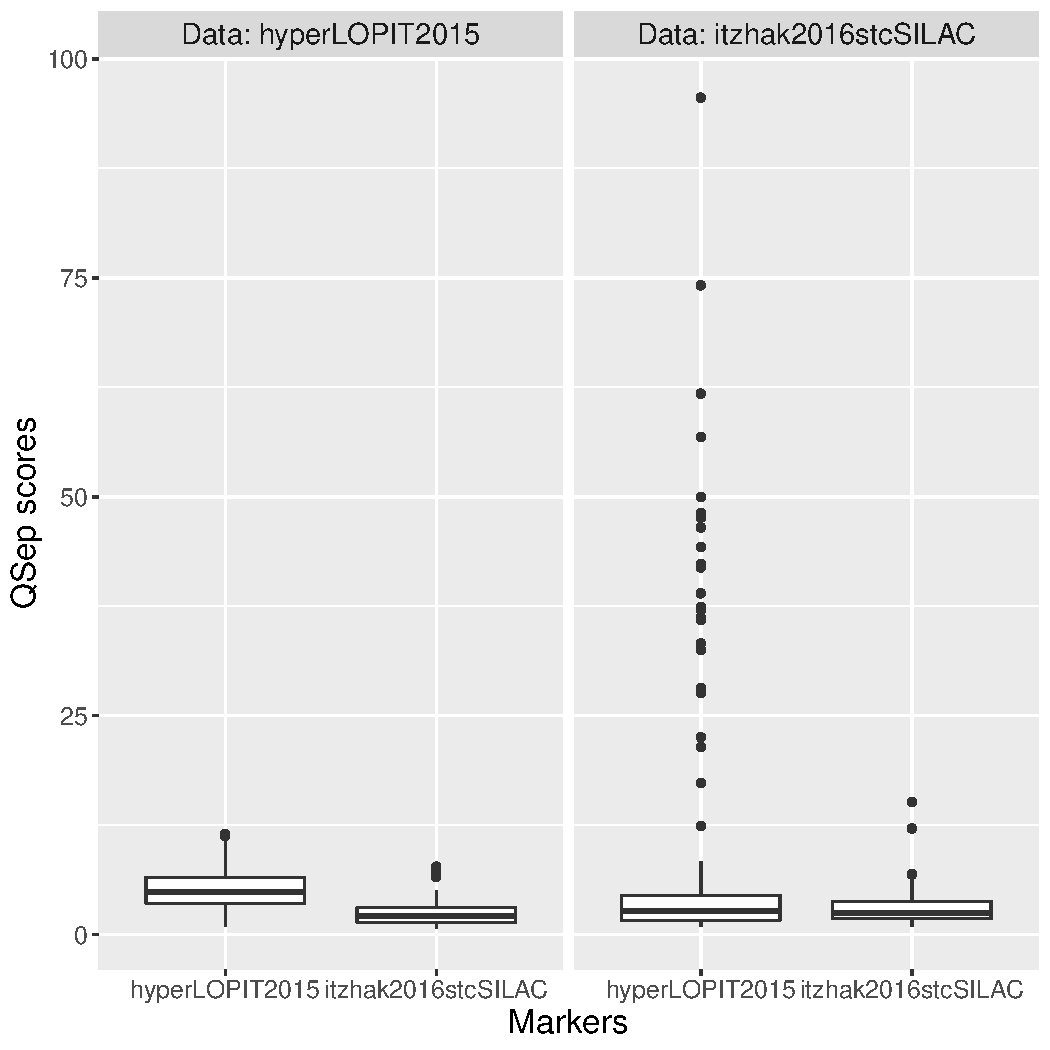
\includegraphics[width = 0.44\textwidth]{mrkswtch-qsep.pdf}}
  \caption{Marker transfer between \textit{hyperLOPIT2015} and
    \textit{itzhak2016stcSILAC}. On the left, the 4 data/marker
    combinations are displayed on PCA plots: the top and bottom row
    contains the \textit{hyperLOPIT2015} and
    \textit{itzhak2016stcSILAC} data respectively, while the left and
    right columns display the markers from \textit{hyperLOPIT2015} and
    \textit{itzhak2016stcSILAC} respectively. On the right, the
    resolution scores have been calculated for the same markers (along
    the $x$ axis) data (left and right panels). Note that the $y$
    scale has been cut at 15, ignoring outlying scores, to focus on
    the bulk of the distribution. }
  \label{fig:mrkswtch}
\end{figure}




As can be seen on figure~\ref{fig:mrkswtch}, transferring the
\textit{itzhak2016stcSILAC} markers to the \textit{hyperLOPIT2015}
dataset has a detrimental effect on the separation (testing the two
distributions with a t-test produces a p-value of \ensuremath{5.1\times 10^{-10}}). Conversely, annotating \textit{itzhak2016stcSILAC} with the
\textit{hyperLOPIT2015} markers significantly improves its resolution
metric (p-value of \ensuremath{1.9\times 10^{-10}}). Comparing both dataset
with the \textit{hyperLOPIT2015} marker set favours the resolution of
the \textit{hyperLOPIT2015} data (p-value of \ensuremath{2.8\times 10^{-4}})
while using the \textit{itzhak2016stcSILAC} markers with the two
datasets substantially reduces their difference in resolution score
(p-value of 0.023).

\section{Conclusions}

In this manuscript, we have described in great detail how to assess
and quantify the resolution of spatial proteomics experiments. We have
applied dimensionality reduction and visualisation, as well as a
simple and intuitive quantitative metric to explore and compare a
variety of publicly available spatial proteomics datasets using the
annotation provided by the original authors. We have also assessed the
resolution metric itself and observed that it was immune to the number
of clusters used for its computation and remained consistent to
different marker annotation.

The ordering of the quantitative resolution detailed in
section~\ref{sec:compara} should not be taken as absolute. Its main
purpose is to provide a guide to compare different experiments. It
will be useful for laboratories that do spatial studies on different
models and with different fractionation and/or quantitation methods,
to assess the impact of these variables (such as, for example
hyperLOPIT MS$^2$ and MS$^3$). It is also useful to compare separation
between different labs, as demonstrated in our comparative study
(section~\ref{sec:compara}). We anticipate that it will also prove
useful for the researcher wanting to assess the resolution of newly
published studies, and put them into a wider context. It is necessary
to emphasise that the importance and effect of marker definition on
estimating and assessing the resolution of spatial proteomics
experiments (section~\ref{sec:qsepassess}) and, of course, the
subsequent assignment of proteins to their most likely sub-cellular
compartments. Sub-cellular resolution is of course only one aspect of
spatial proteomics, albeit am important one, that critically
determines the reliability of protein assignments to spatial niches as
well as the identification of multi- and trans-localisation events.

\bigskip

Finally, we reflect on the implications of this work on the spatial
proteomics community, and more generally the cell biology community
that relies on protein localisation data. We have assessed dataset
spanning 12 years of spatial proteomics. Since 2006, the community has
seen many important improvements: tremendous advances in mass
spectrometry, improvements in spatial proteomics designs, and
considerable breakthroughs in data analysis. One might then wonder
whether these benefits have lead to tangible improvements in
resolution over time?

On figure~\ref{fig:restime}, we have ordered the datasets' resolution
metric according to their publication year. We can see that a set of
recent datasets, including the mouse stem cell
\citep{Christoforou:2016} and U2OS \citep{Thul:2017} hyperLOPIT
experiments (published in 2016 and 2017 respectively), and a variation
thereof, where \citet{JeanBeltran:2016} (published in 2016),
incorporating a temporal component in their experimental design, show
a consistent superior resolution.

\begin{figure}[h]
  \centering
\begin{knitrout}
\definecolor{shadecolor}{rgb}{0.969, 0.969, 0.969}\color{fgcolor}
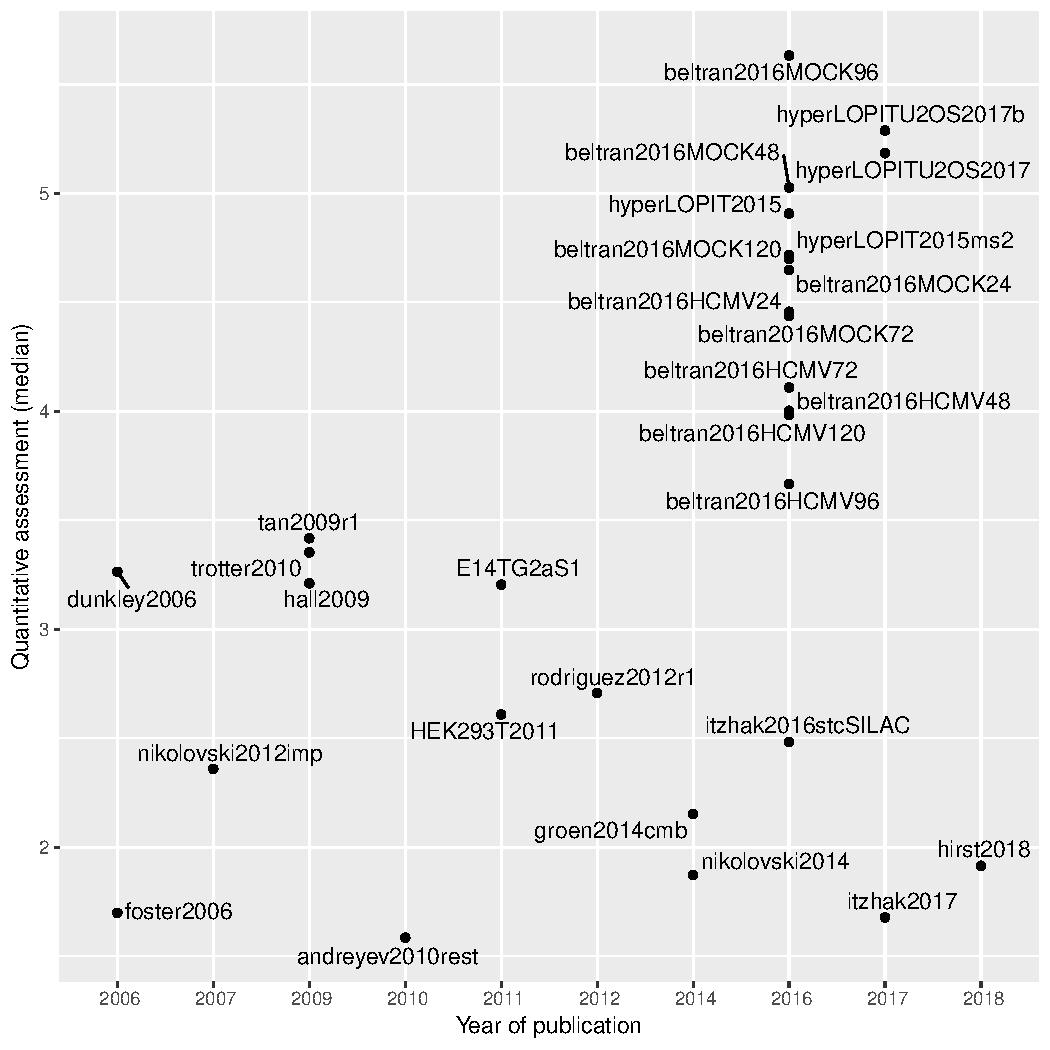
\includegraphics[width=0.8\linewidth]{figure/restime-1} 

\end{knitrout}
\caption{Resolution of spatial proteomics experiments over time. The
  assigned dates match either the original publication or, when know,
  the actual date the data was generated. For publications that
  re-analysed data, the date of the original publication of generation
  was used. When publications used several datasets, the date of the
  most recent one was used.}
  \label{fig:restime}
\end{figure}


While the definition of sub-cellular resolution, as defined by the
QSep measure, is only one aspect of spatial proteomics, one could
argue that the community at large would benefit from a more systematic
approach when considering the resolution of spatial proteomics
experiments. Indeed, there are various aspects that can be worked on
to improve resolution: quantitation accuracy at the mass spectrometry
level (see figures~\ref{fig:density} and~\ref{fig:hexbin1} comparing
SPS MS$^3$ and conventional MS$^2$ for an example), optimisations in
sub-cellular fractionation (as exemplified by the substantial
improvement obtained by \citep{Christoforou:2016}), improved data
annotation (see for example figure~\ref{fig:mrkswtch}), as well as
superior data analysis (for example using semi-supervised learning
\citet{Breckels:2013}).

Maybe there a need for some standardisation, or some general
guidelines in assessing spatial proteomics data in the community?
Shouldn't the community as a whole aim for collective improvement and
some agreement as to what constitutes a good spatial proteomics
experiment and a reliable protein sub-cellular assignment? The latter
can assessed using improved probabilistic classifiers such as the
Bayesian mixture modelling approach proposed by \citet{Crook:2018}. In
this work, we propose the QSep metric to assess the former. Better
spatial proteomics data and more reliable interpretation will be of
direct benefit to the spatial proteomics researchers themselves, and
will increase the trust and reliance of the cell biology community.

\section*{Acknowledgements}

This work was supported by a BBSRC Strategic Longer and Larger grant
(Award BB/L002817/1), a Wellcome Trust Technology Development Grant
(Grant number 108441/Z/15/Z) and a BBSRC Tools and resources
development grant (Award BB/N023129/1). The authors would like to
thank Dr Claire M. Mulvey for helpful comments on the quantitative
assessment.

\section*{Author contributions}

LG conceptualised the method and wrote the initial manuscript
draft. LG and LMB developed the QSep code. KSL contributed datasets
and feedback. All authors read and approved the manuscript.

\newpage

\begin{appendices}

\section{Additional figures}\label{sec:figs}

This section shows the density and annotated PCA and QSep plots for
the 29 datasets showcased in this manuscript.

\begin{figure}[htb]
  \centering
  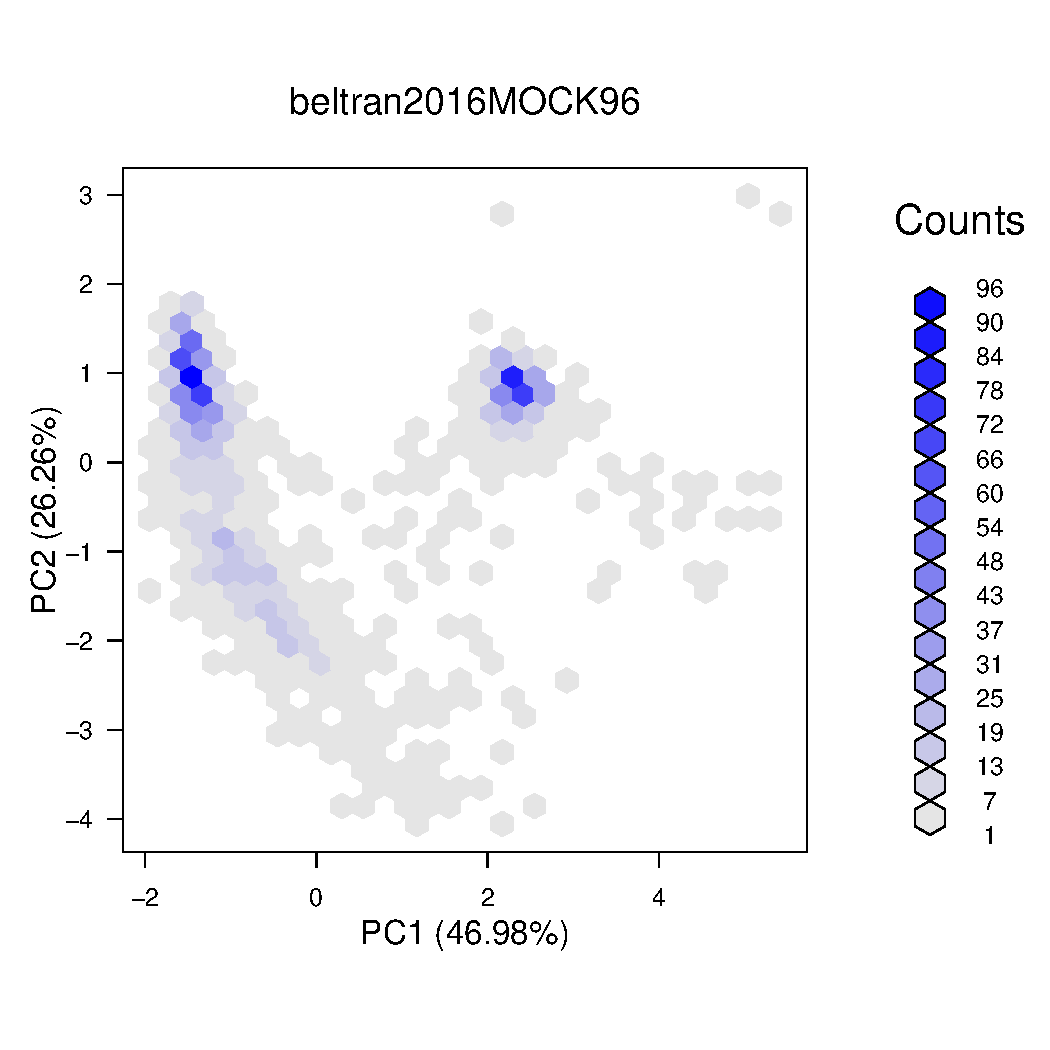
\includegraphics[width = 0.32\textwidth]{./figure/fighexpca-1.pdf}
  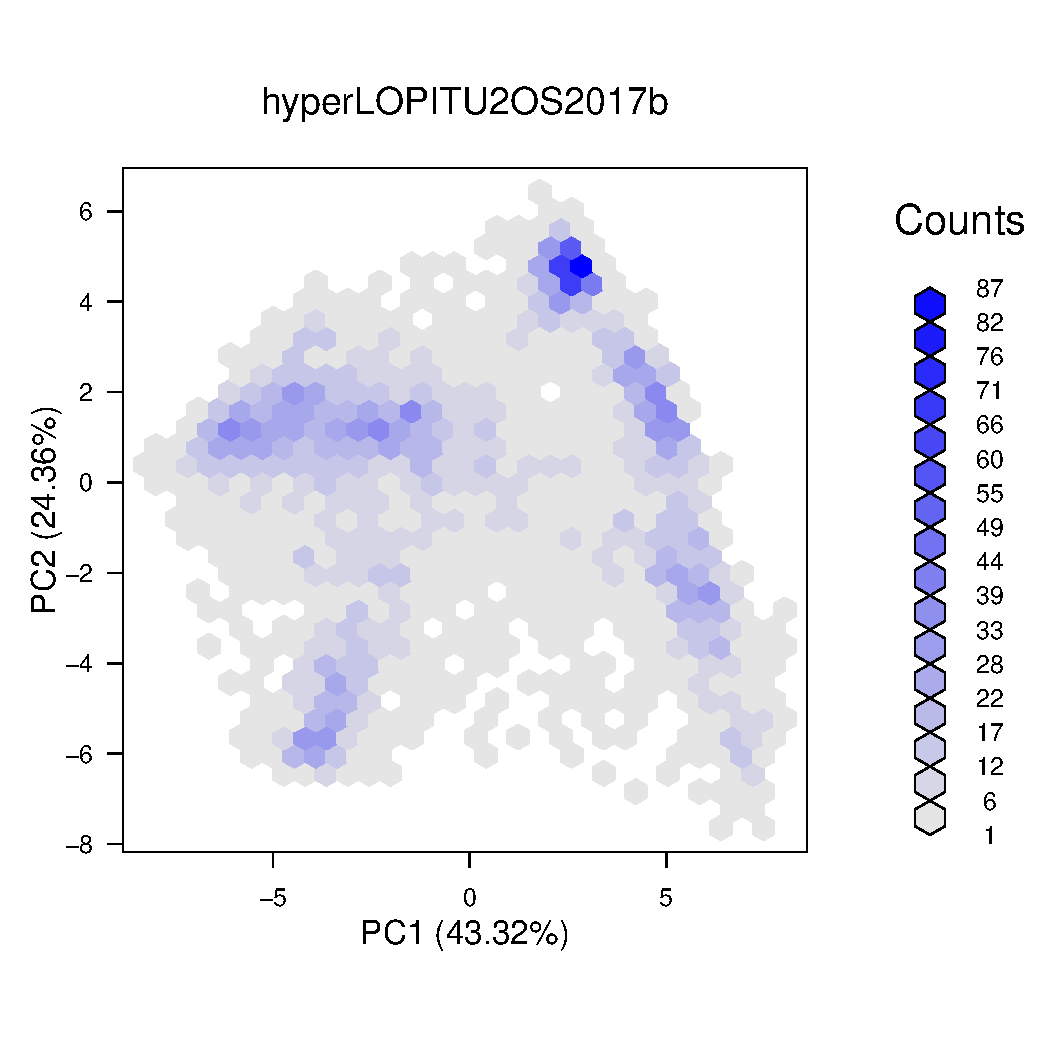
\includegraphics[width = 0.32\textwidth]{./figure/fighexpca-2.pdf}
  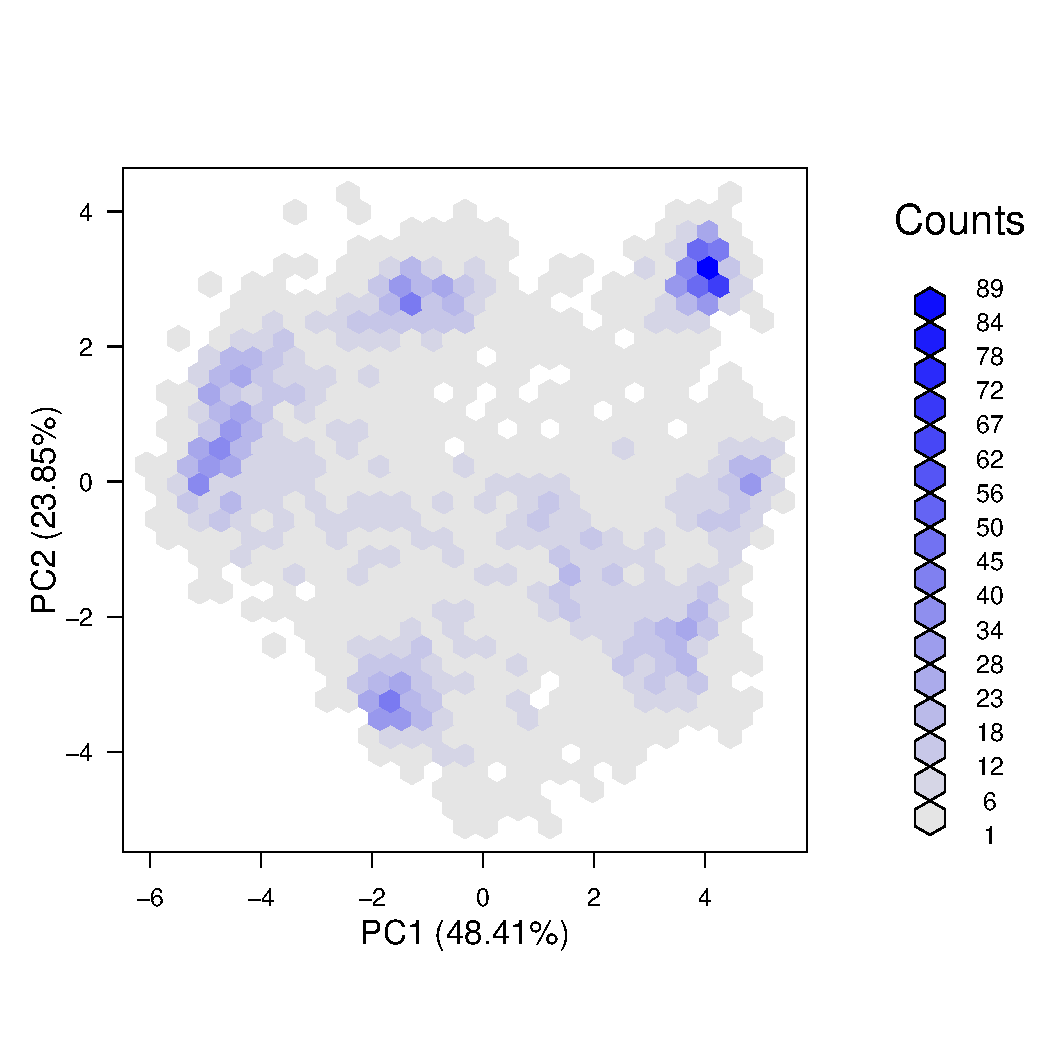
\includegraphics[width = 0.32\textwidth]{./figure/fighexpca-3.pdf}
  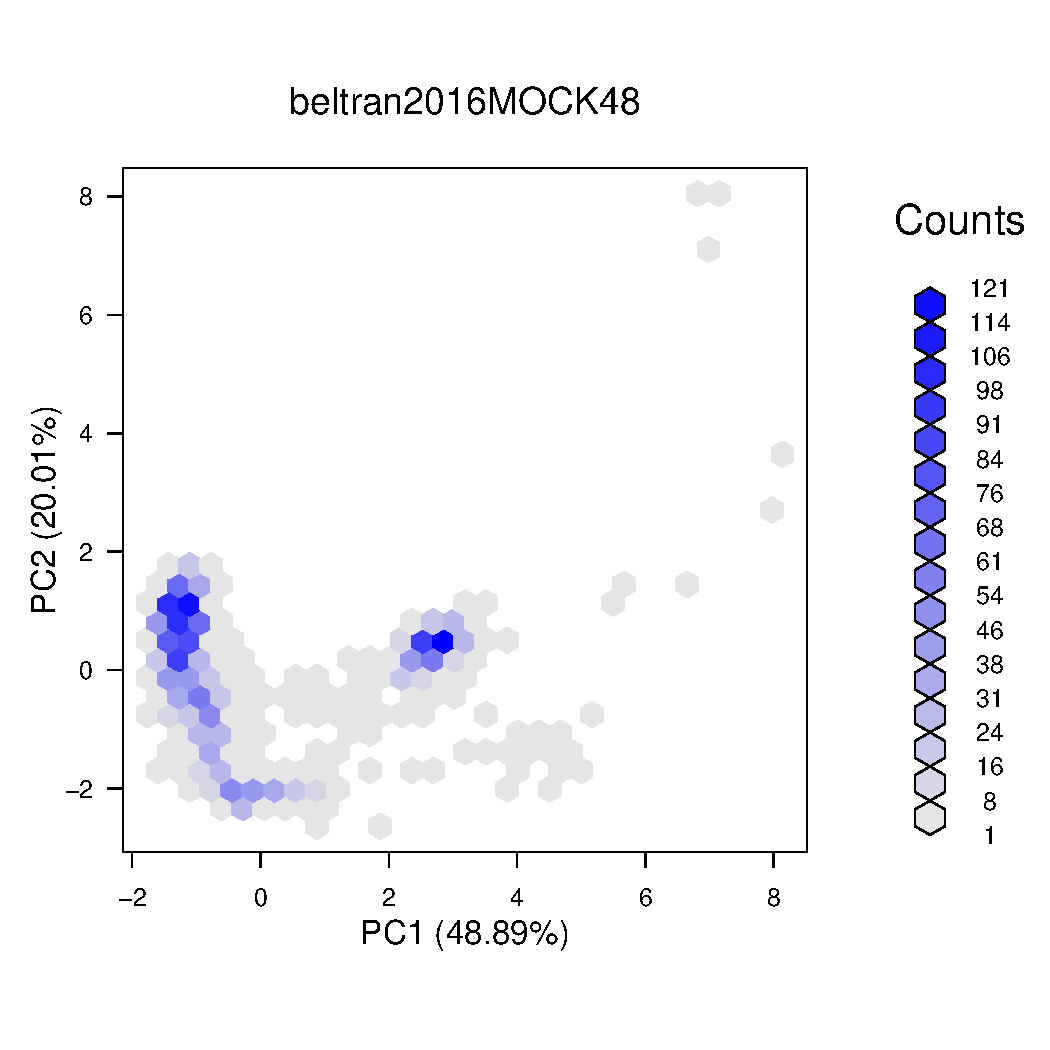
\includegraphics[width = 0.32\textwidth]{./figure/fighexpca-4.pdf}
  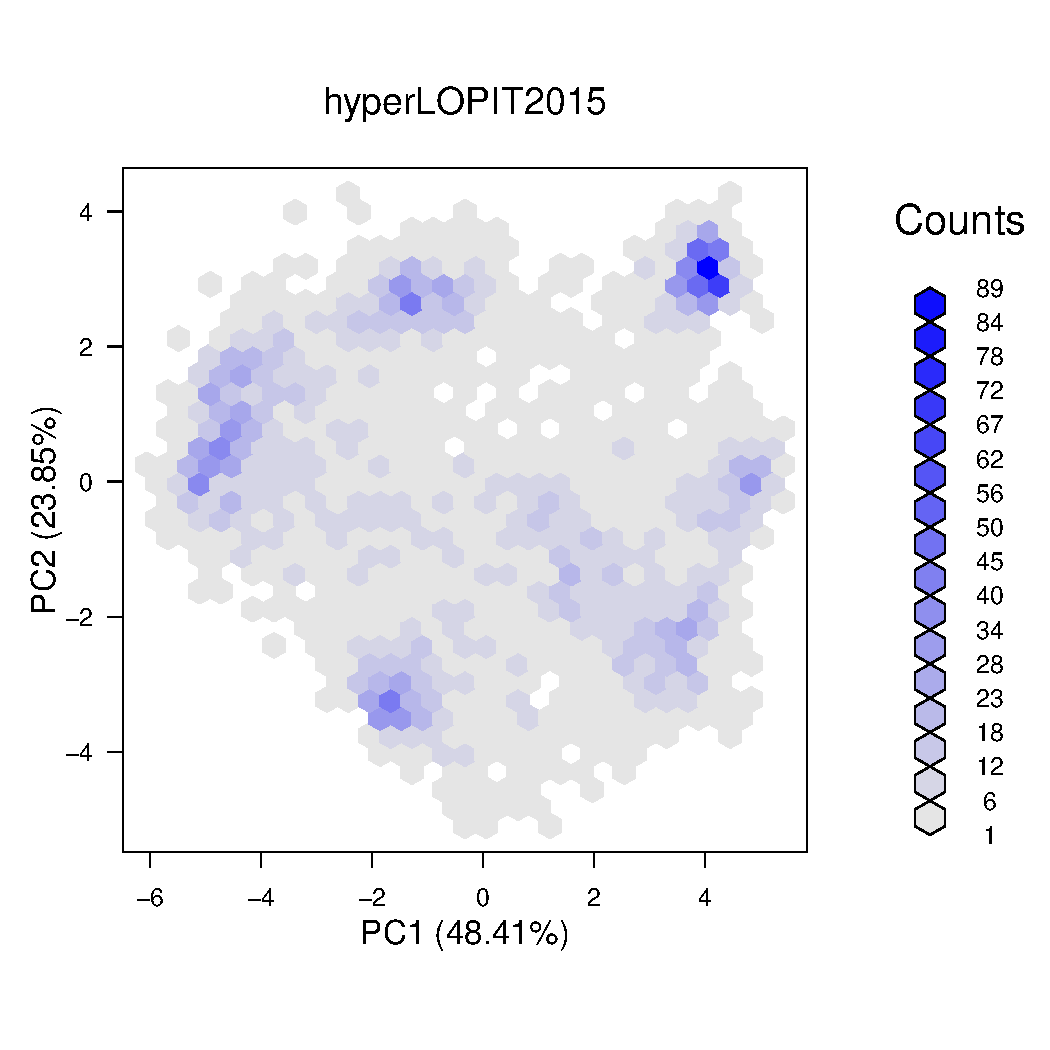
\includegraphics[width = 0.32\textwidth]{./figure/fighexpca-5.pdf}
  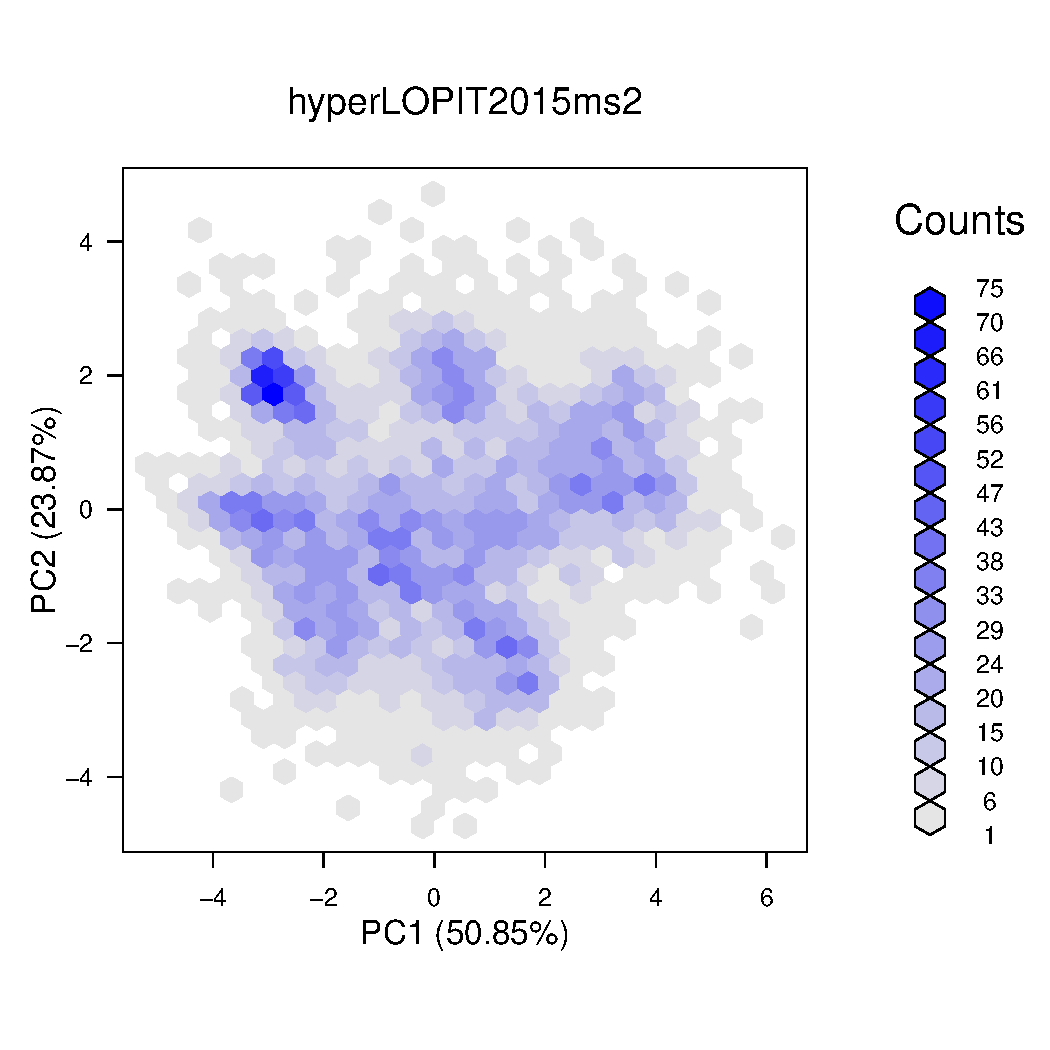
\includegraphics[width = 0.32\textwidth]{./figure/fighexpca-6.pdf}
  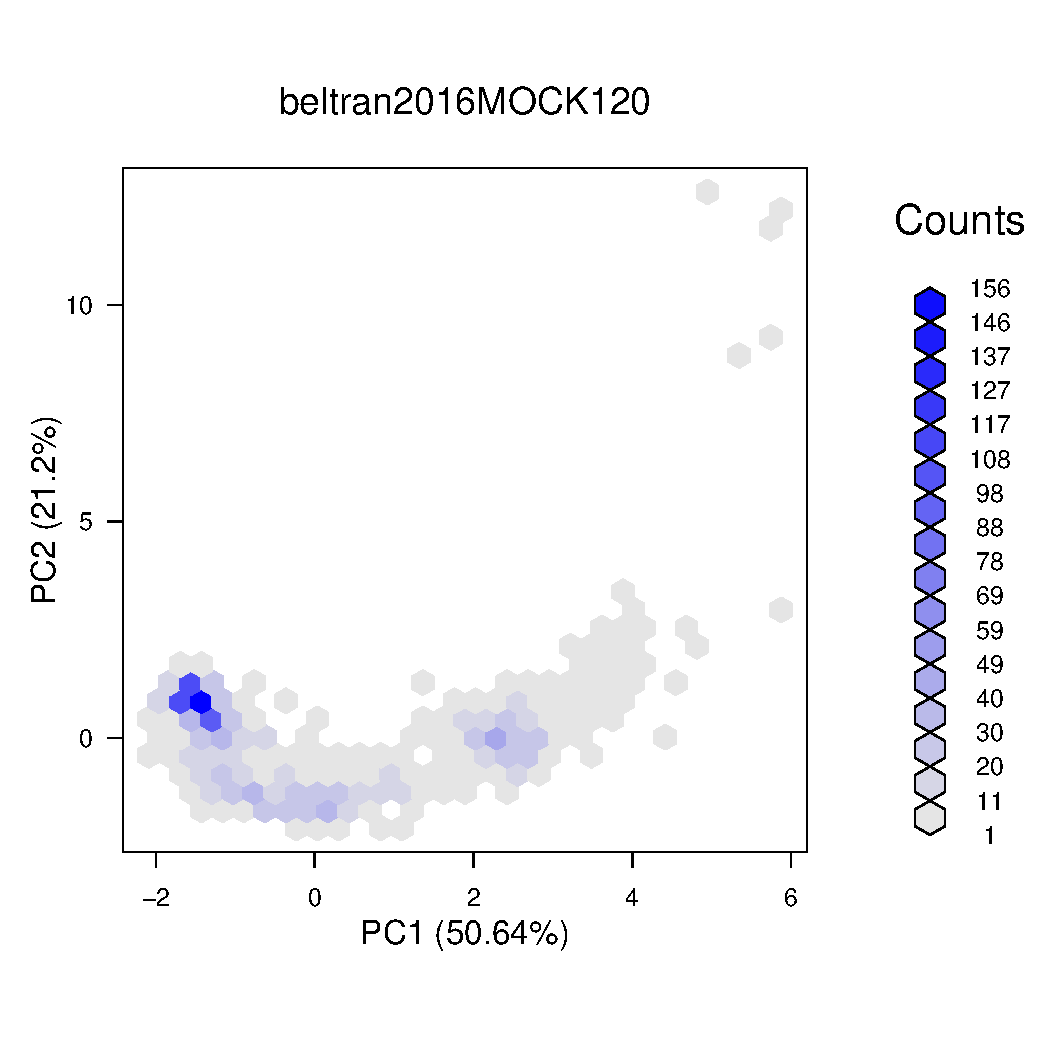
\includegraphics[width = 0.32\textwidth]{./figure/fighexpca-7.pdf}
  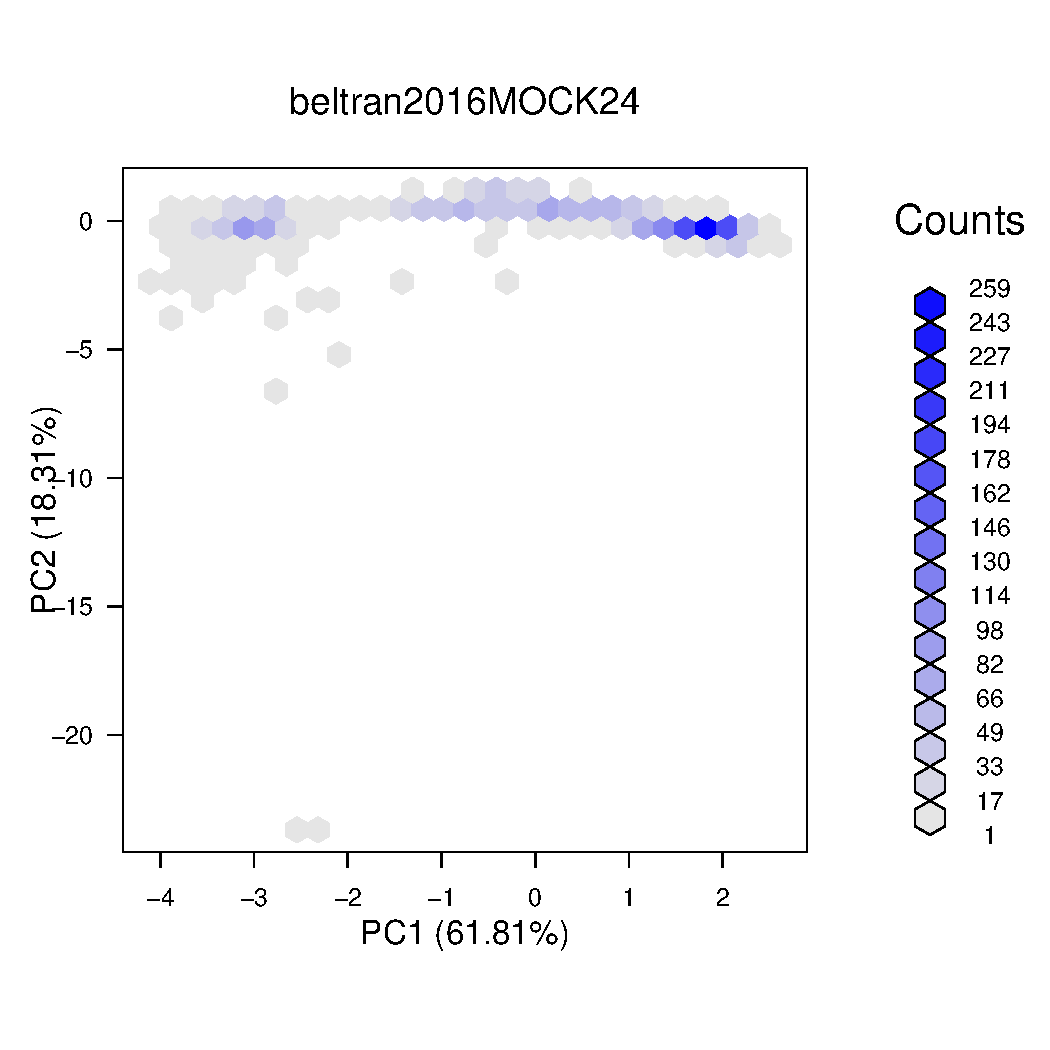
\includegraphics[width = 0.32\textwidth]{./figure/fighexpca-8.pdf}
  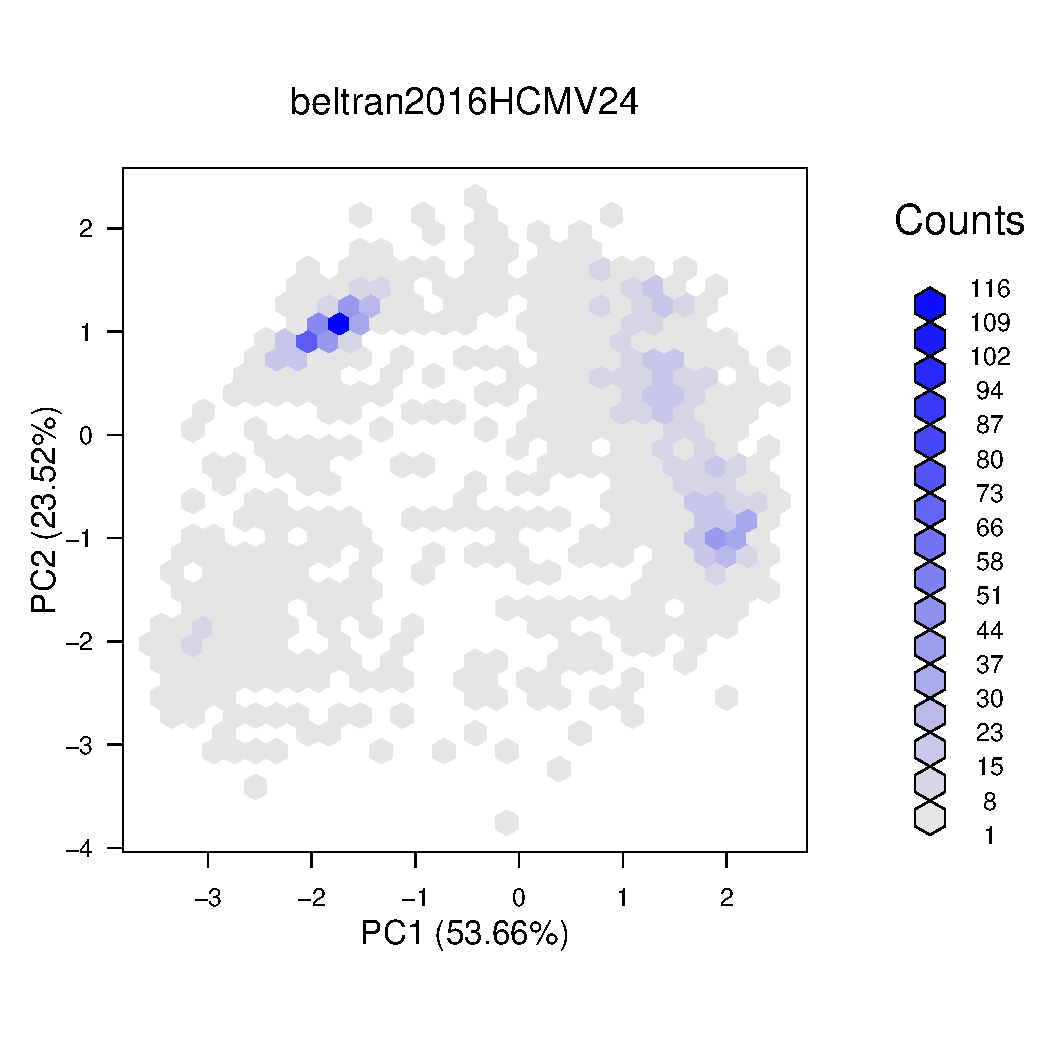
\includegraphics[width = 0.32\textwidth]{./figure/fighexpca-9.pdf}
\end{figure}
\begin{figure}[htb]\ContinuedFloat
  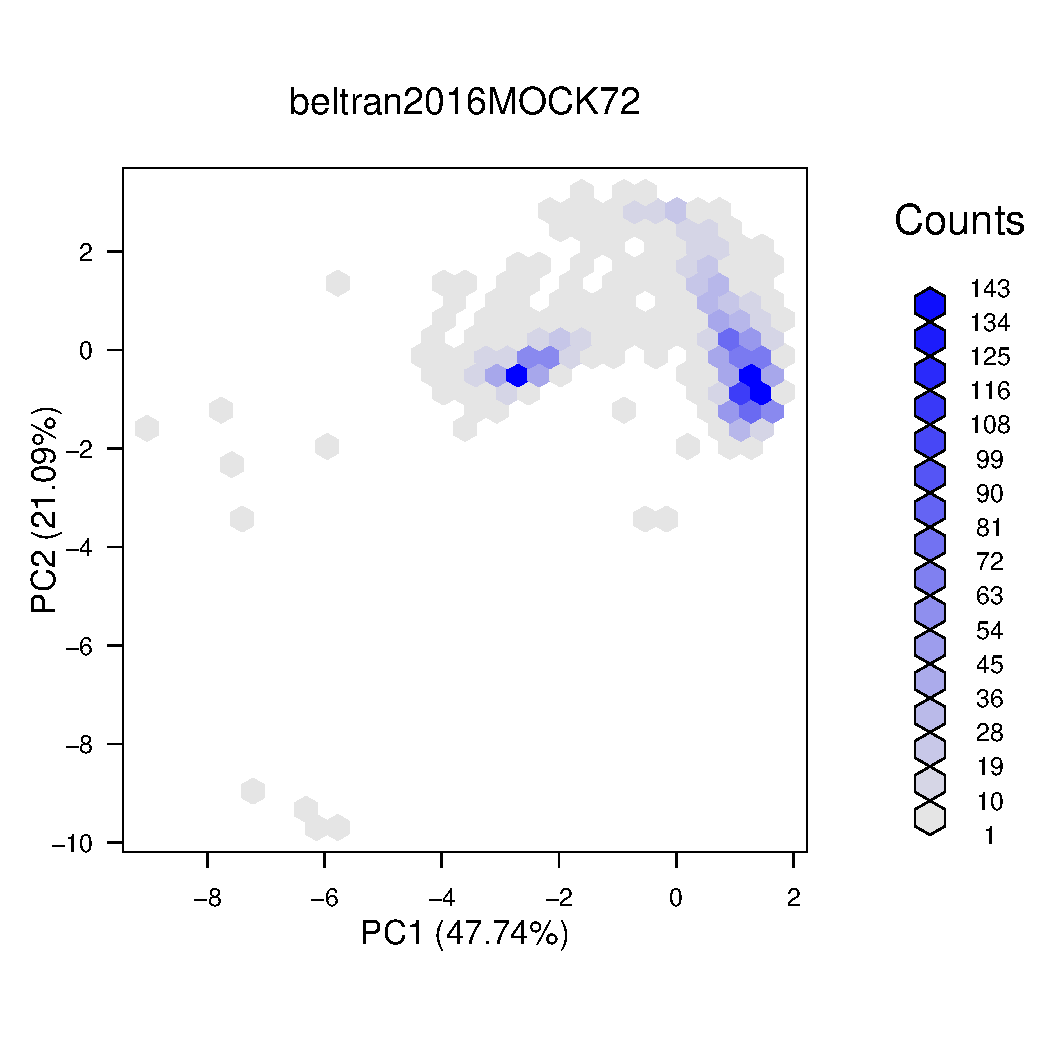
\includegraphics[width = 0.32\textwidth]{./figure/fighexpca-10.pdf}
  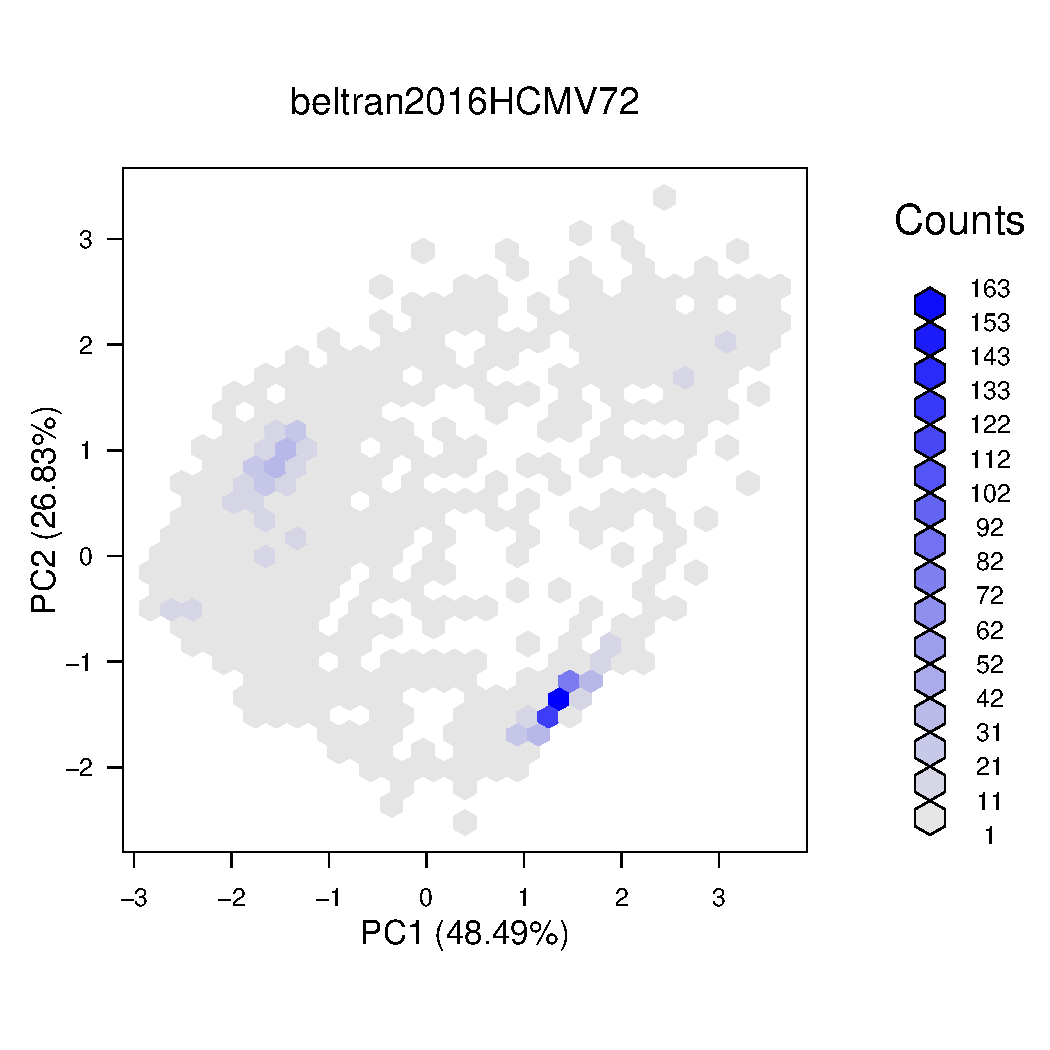
\includegraphics[width = 0.32\textwidth]{./figure/fighexpca-11.pdf}
  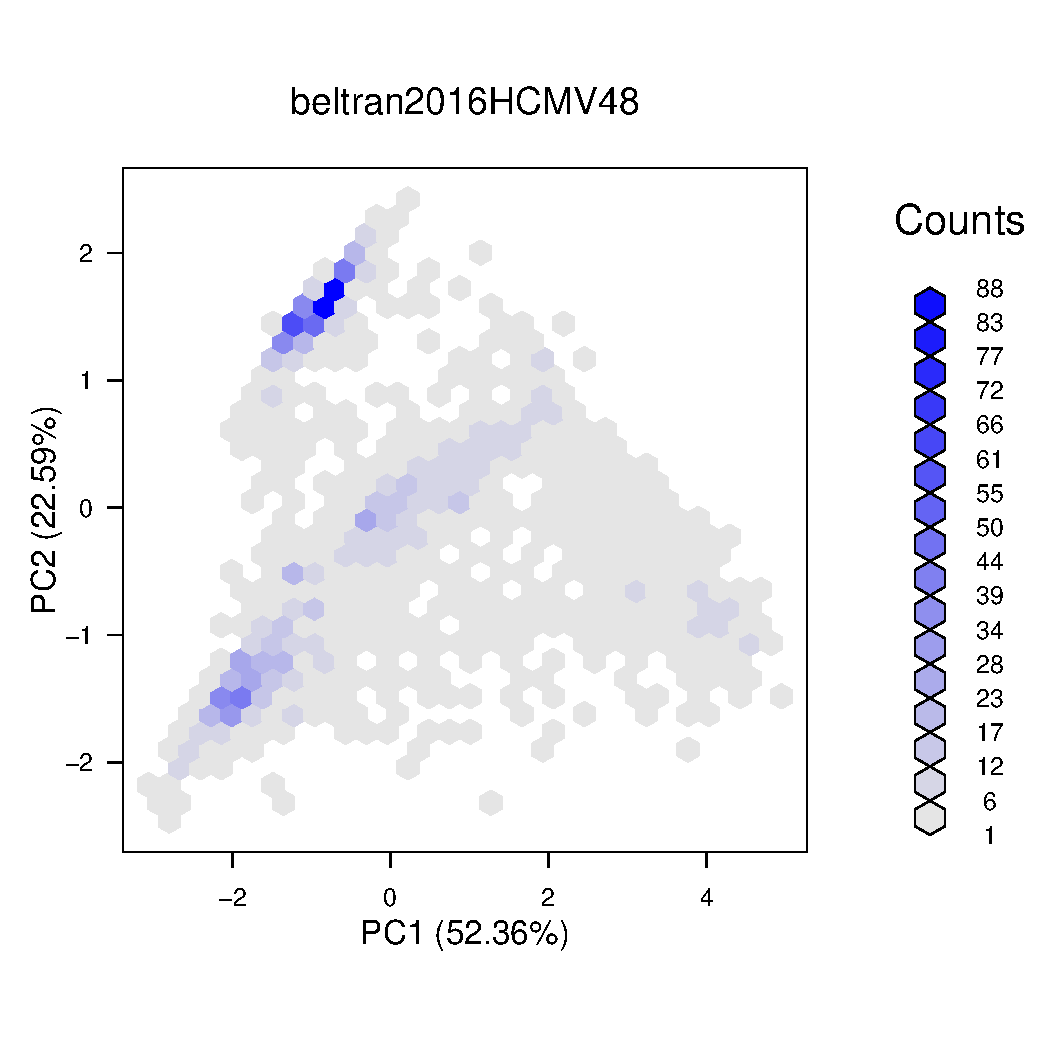
\includegraphics[width = 0.32\textwidth]{./figure/fighexpca-12.pdf}
  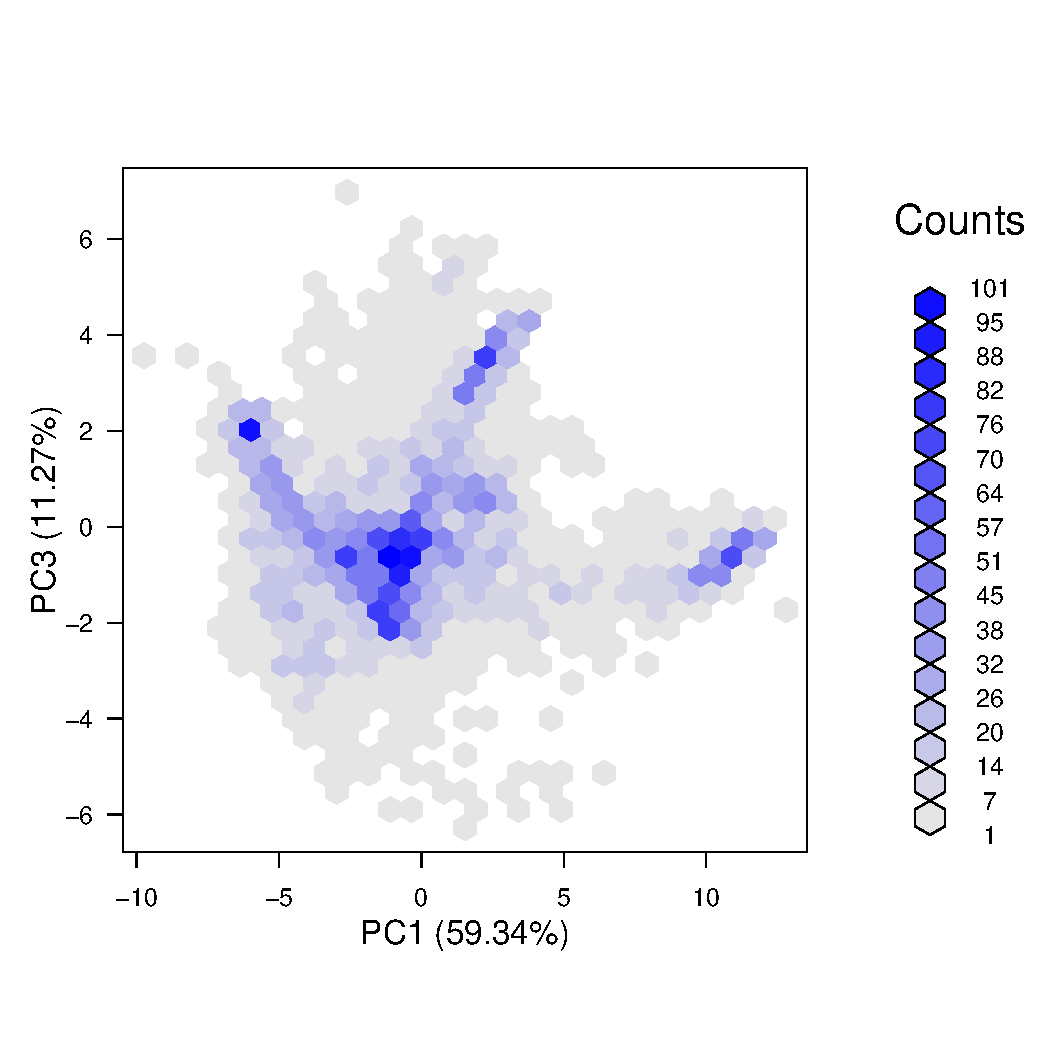
\includegraphics[width = 0.32\textwidth]{./figure/fighexpca-13.pdf}
  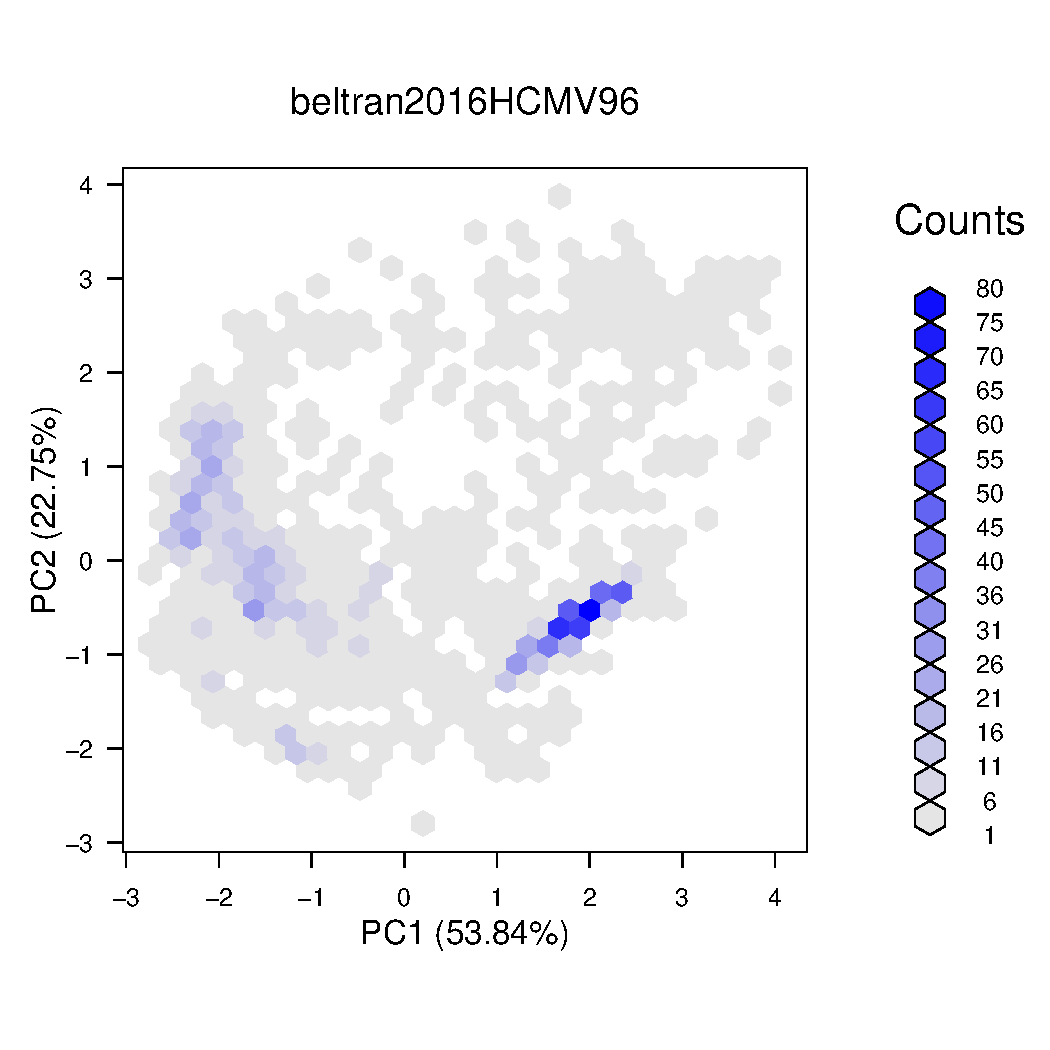
\includegraphics[width = 0.32\textwidth]{./figure/fighexpca-14.pdf}
  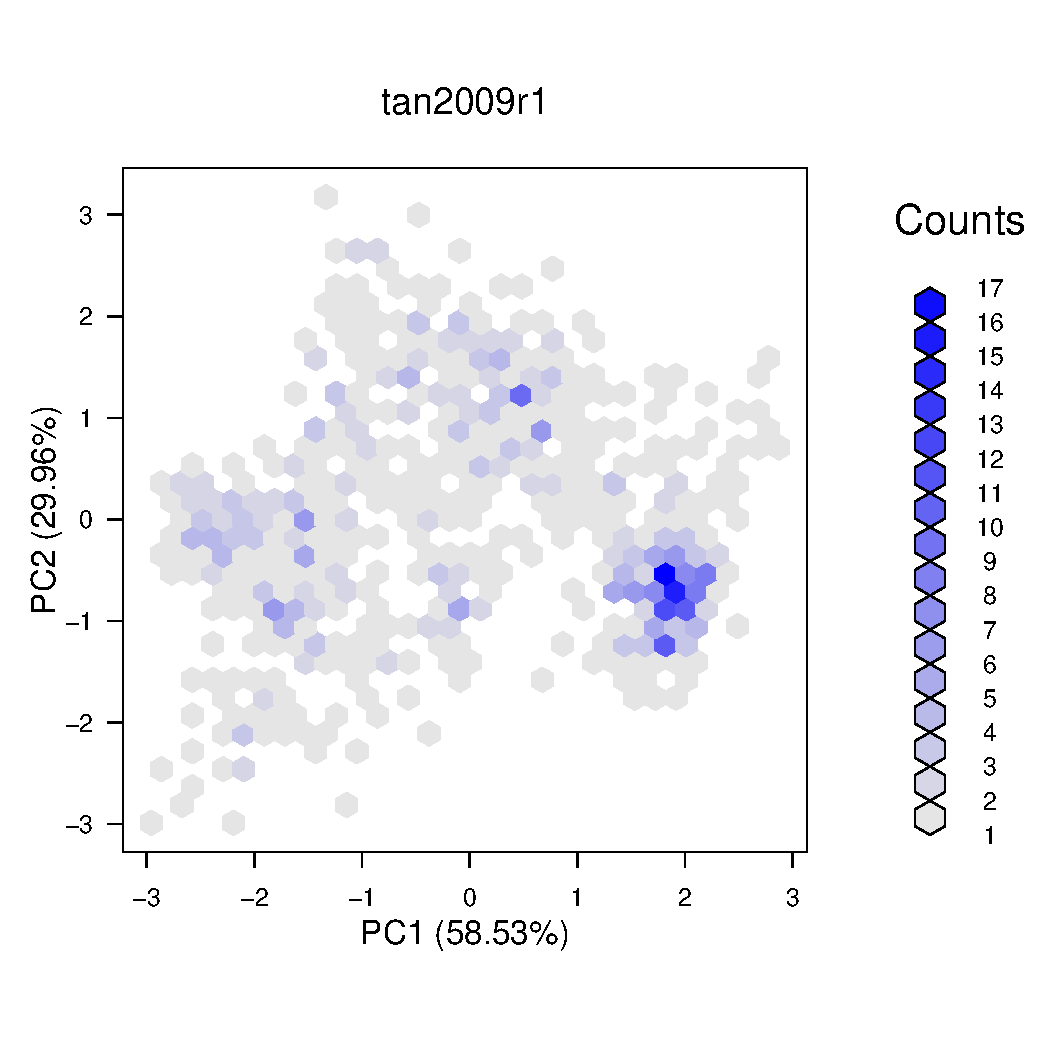
\includegraphics[width = 0.32\textwidth]{./figure/fighexpca-15.pdf}
  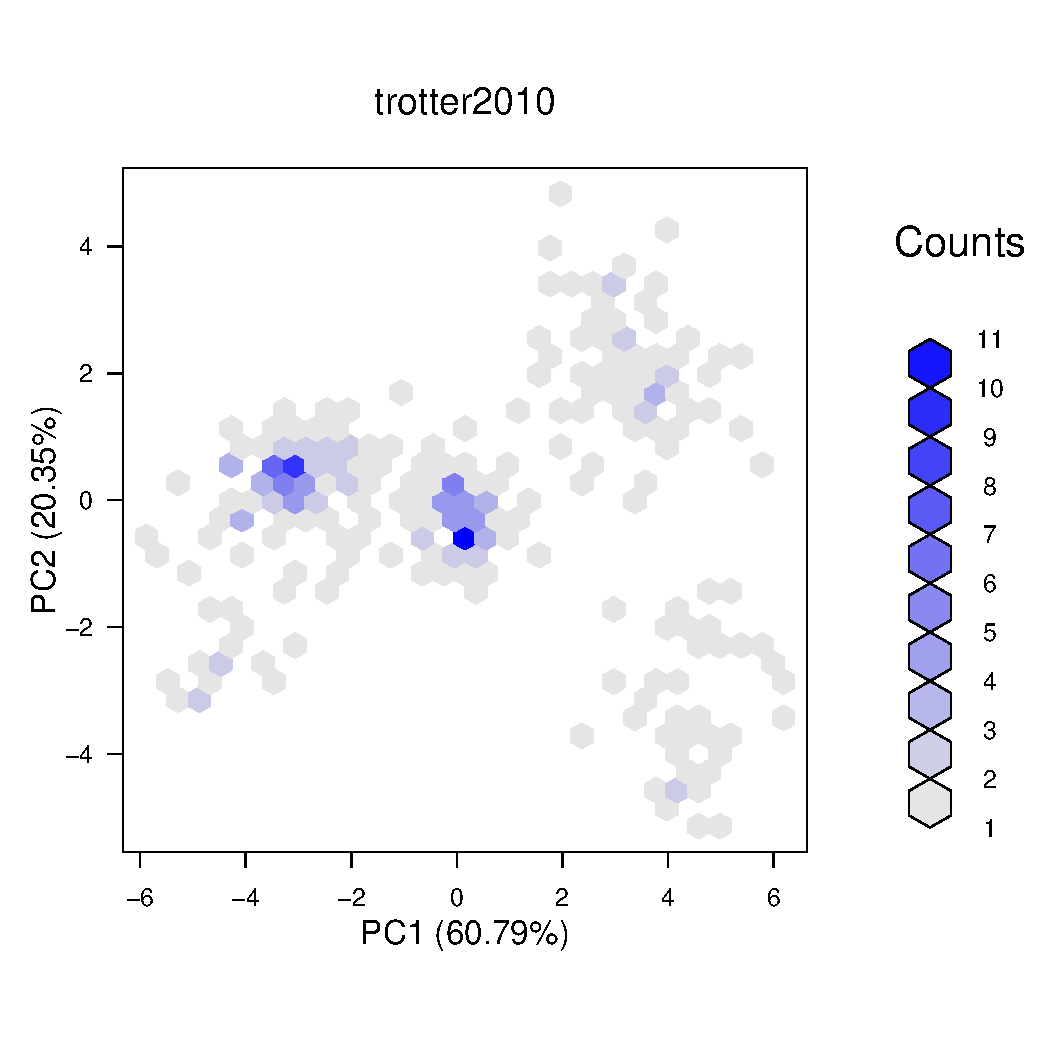
\includegraphics[width = 0.32\textwidth]{./figure/fighexpca-16.pdf}
  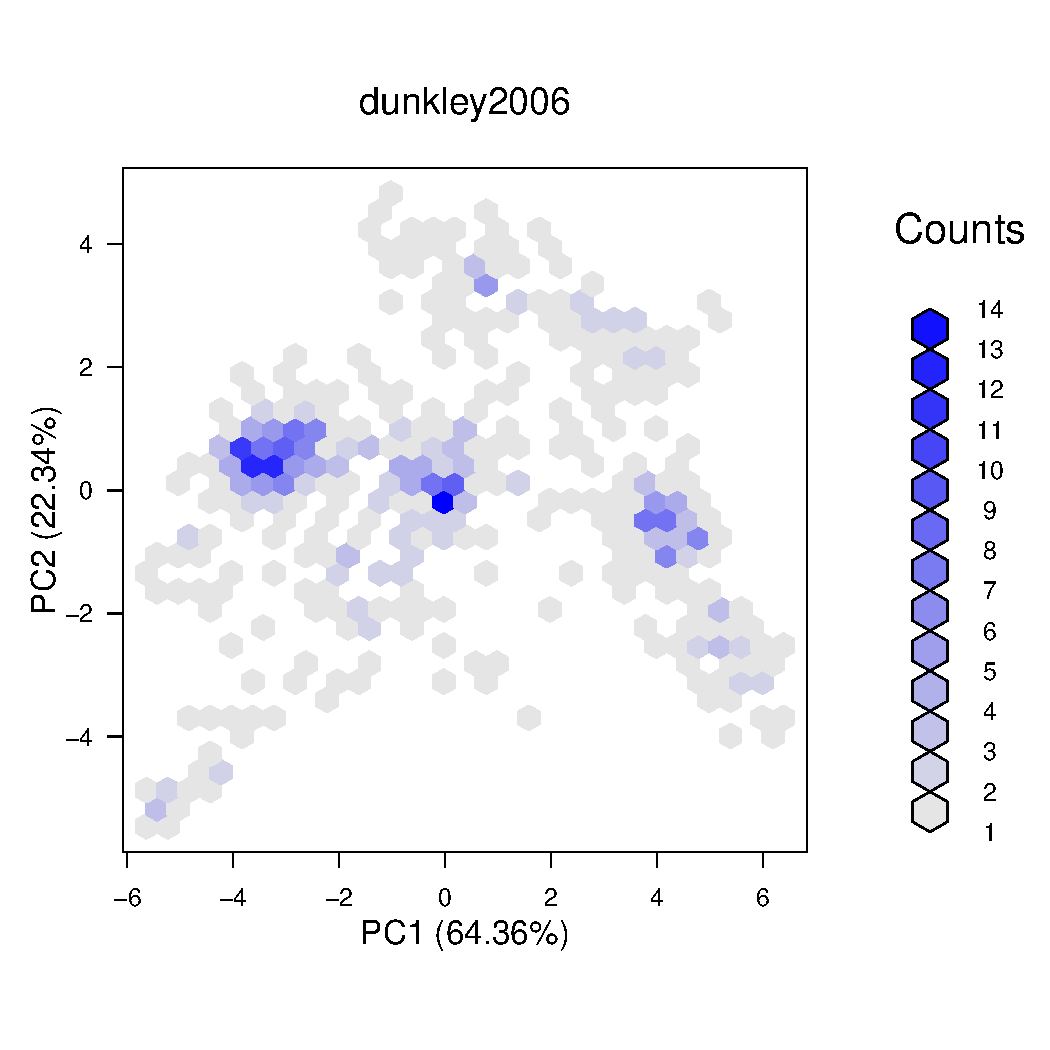
\includegraphics[width = 0.32\textwidth]{./figure/fighexpca-17.pdf}
  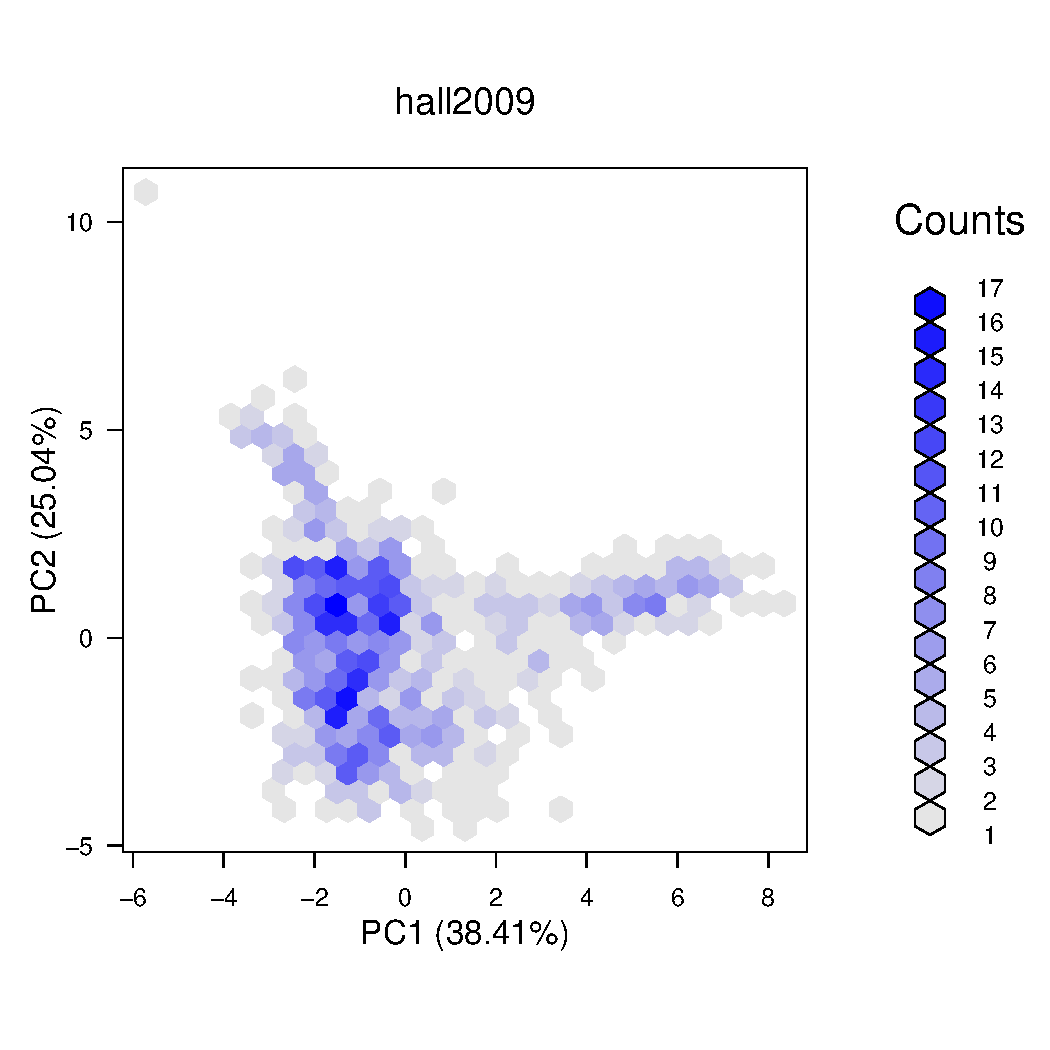
\includegraphics[width = 0.32\textwidth]{./figure/fighexpca-18.pdf}
  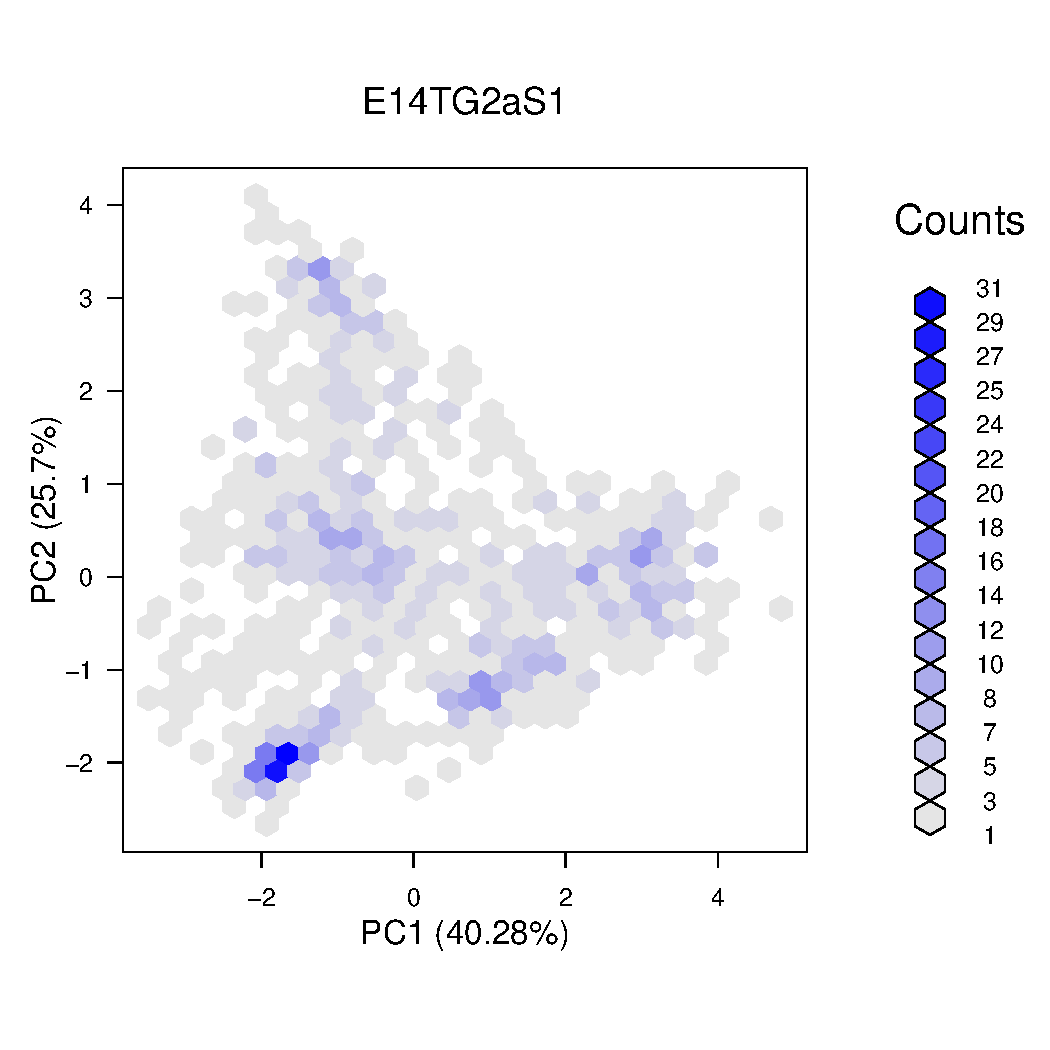
\includegraphics[width = 0.32\textwidth]{./figure/fighexpca-19.pdf}
  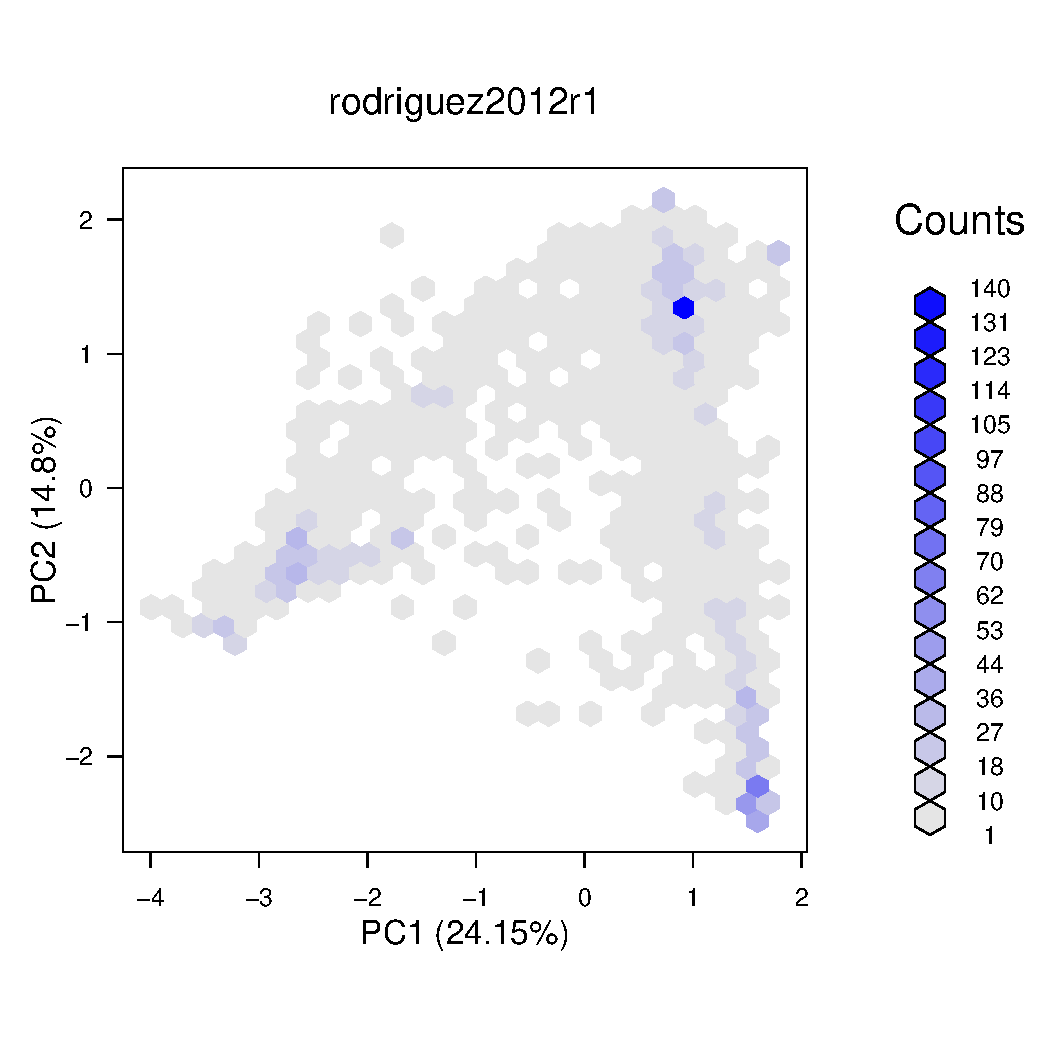
\includegraphics[width = 0.32\textwidth]{./figure/fighexpca-20.pdf}
  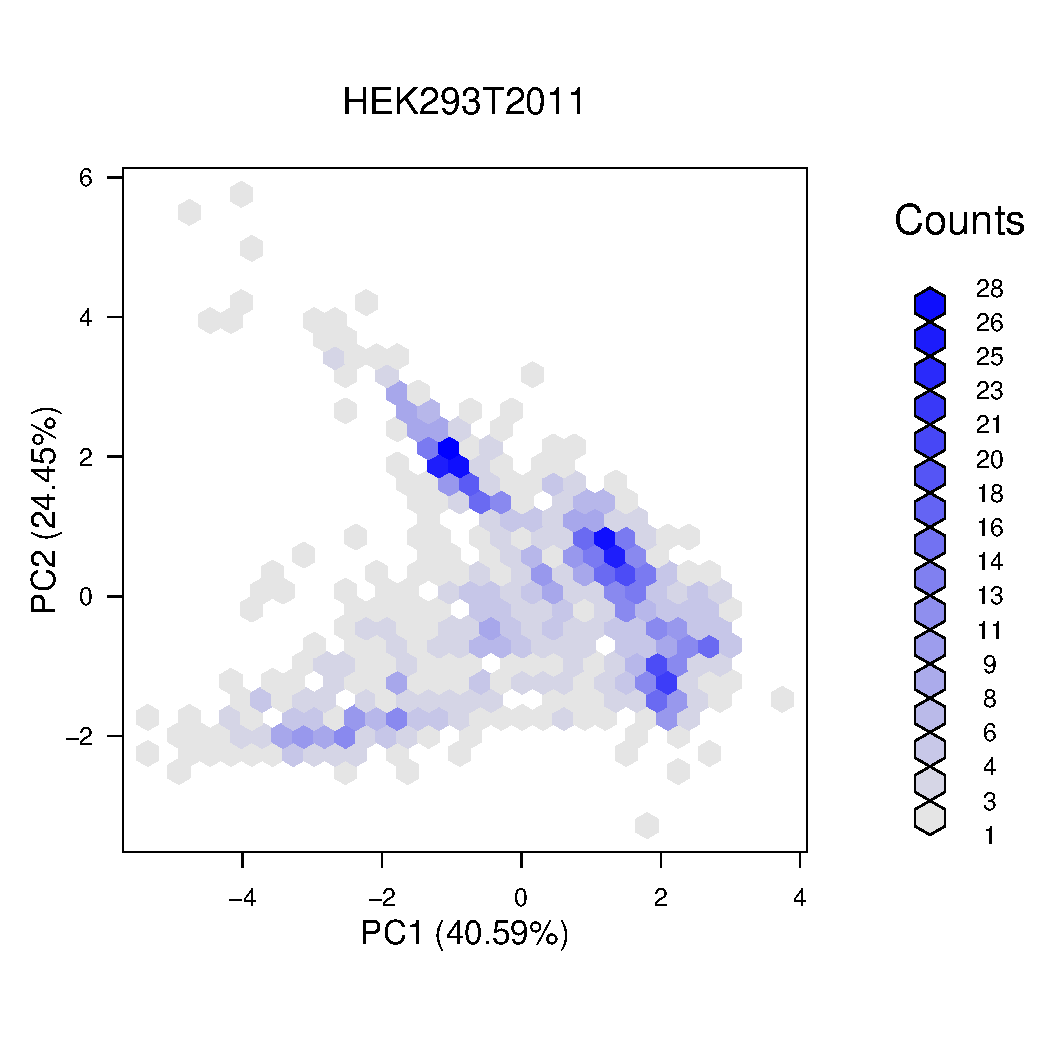
\includegraphics[width = 0.32\textwidth]{./figure/fighexpca-21.pdf}
\end{figure}
\begin{figure}[htb]
  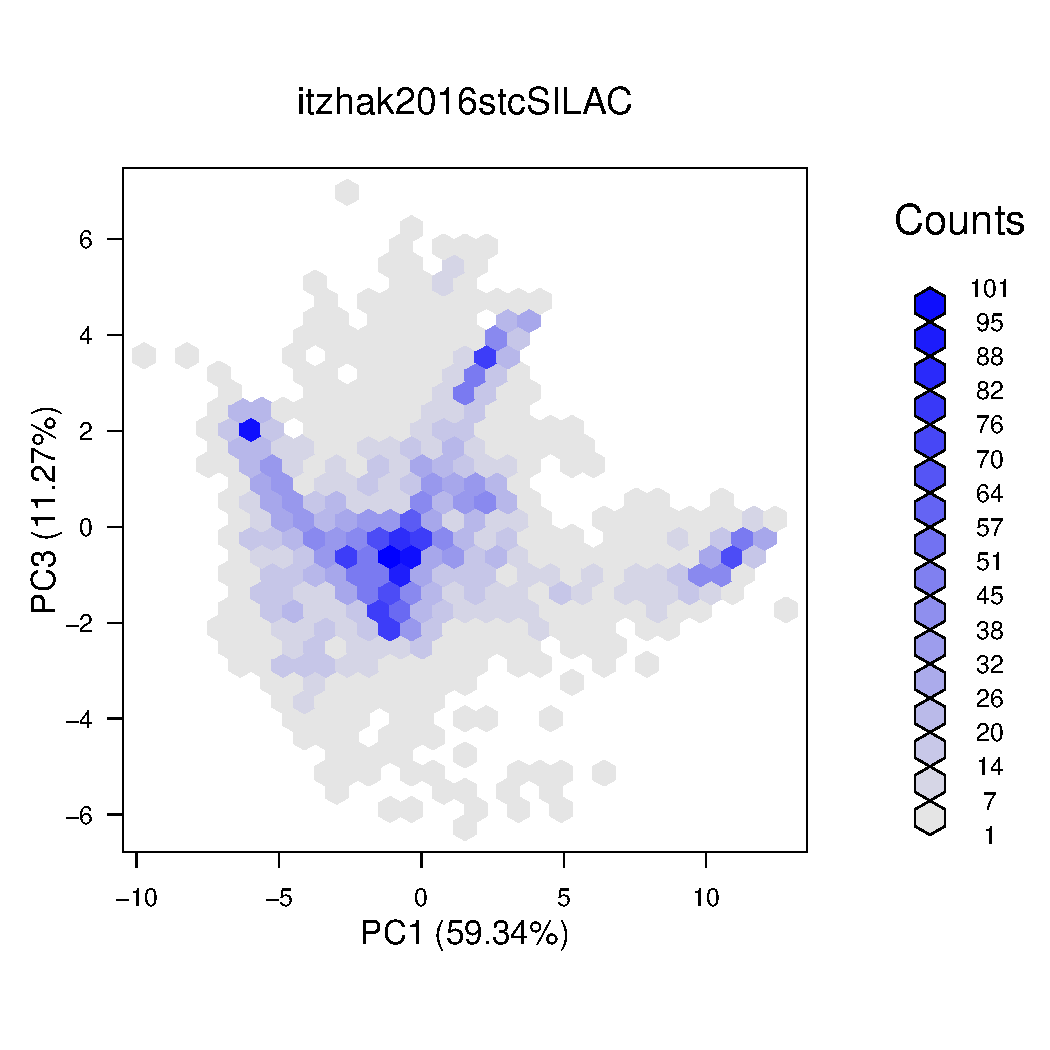
\includegraphics[width = 0.32\textwidth]{./figure/fighexpca-22.pdf}
  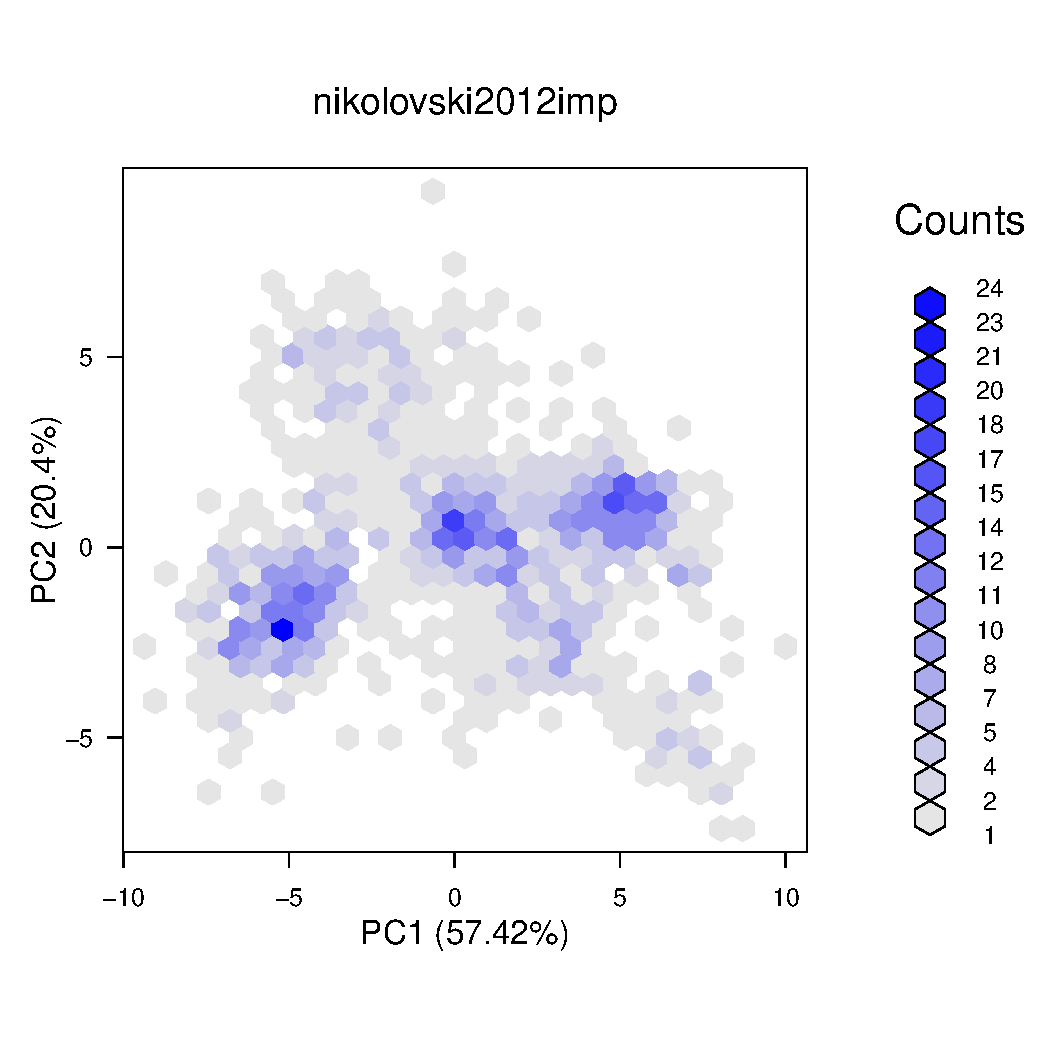
\includegraphics[width = 0.32\textwidth]{./figure/fighexpca-23.pdf}
  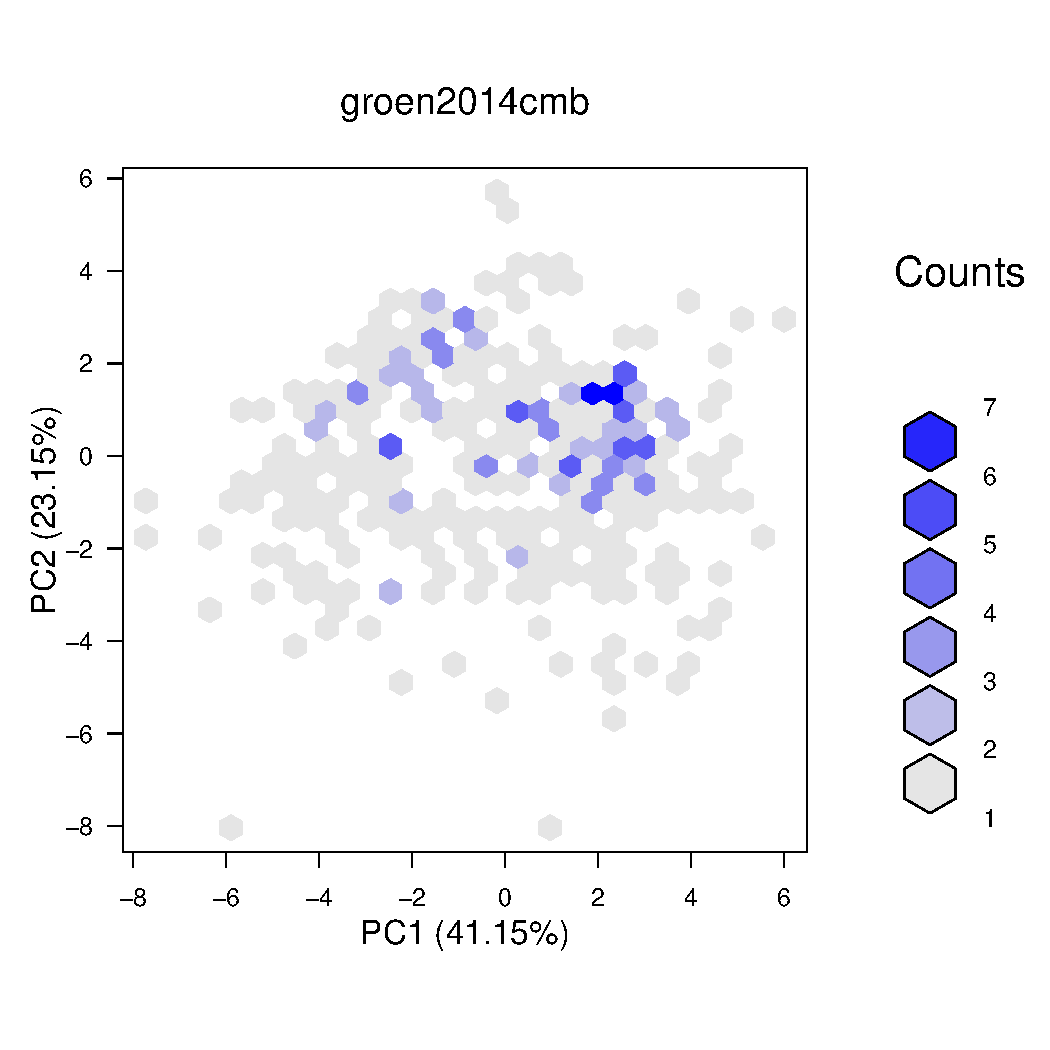
\includegraphics[width = 0.32\textwidth]{./figure/fighexpca-24.pdf}
  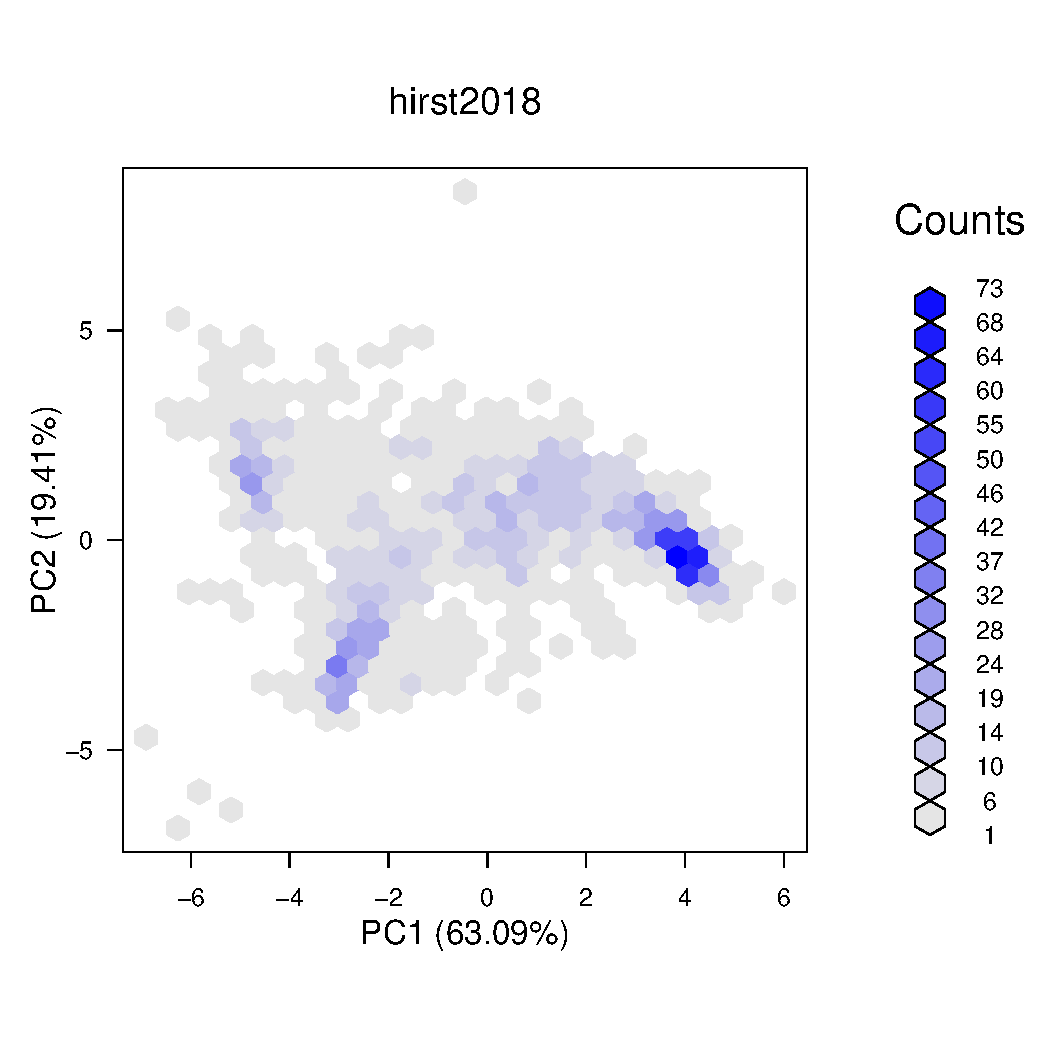
\includegraphics[width = 0.32\textwidth]{./figure/fighexpca-25.pdf}
  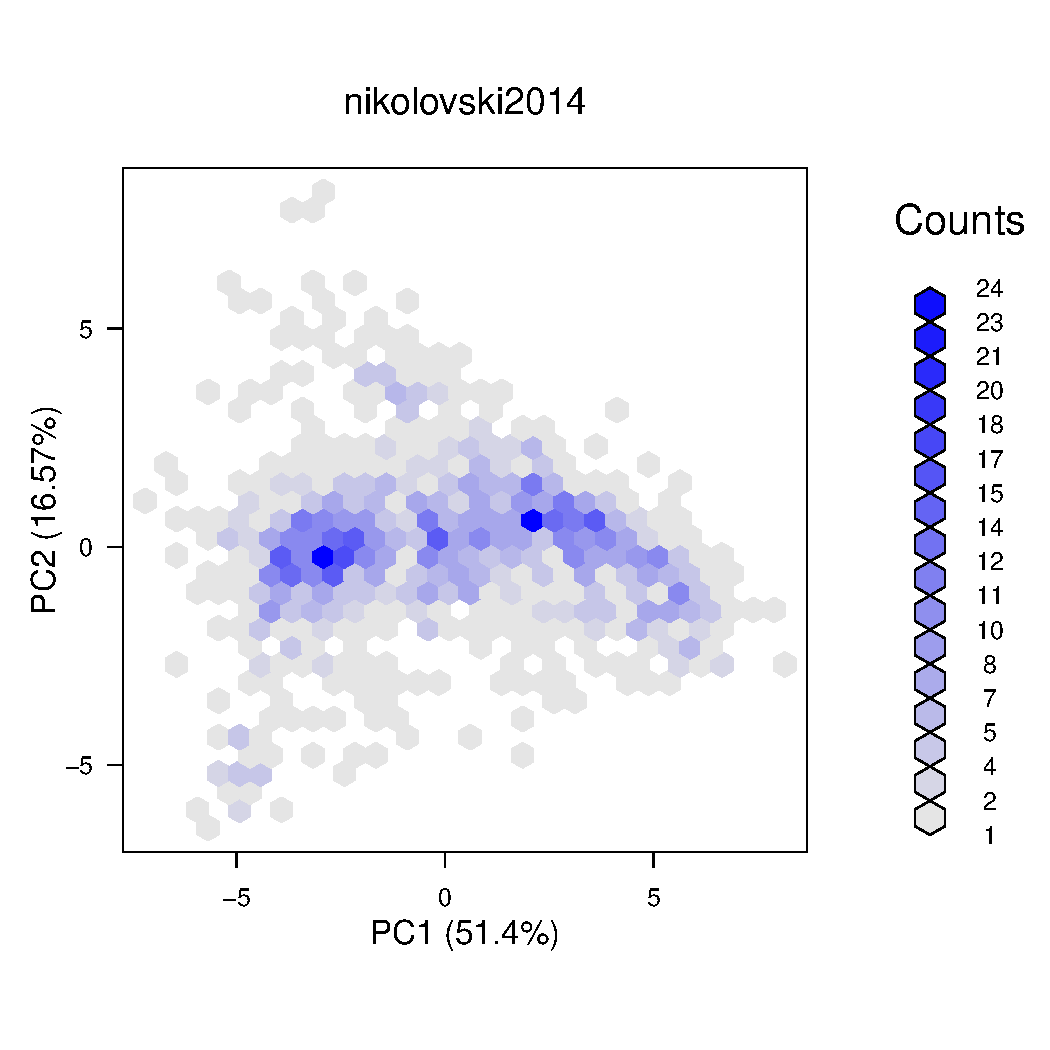
\includegraphics[width = 0.32\textwidth]{./figure/fighexpca-26.pdf}
  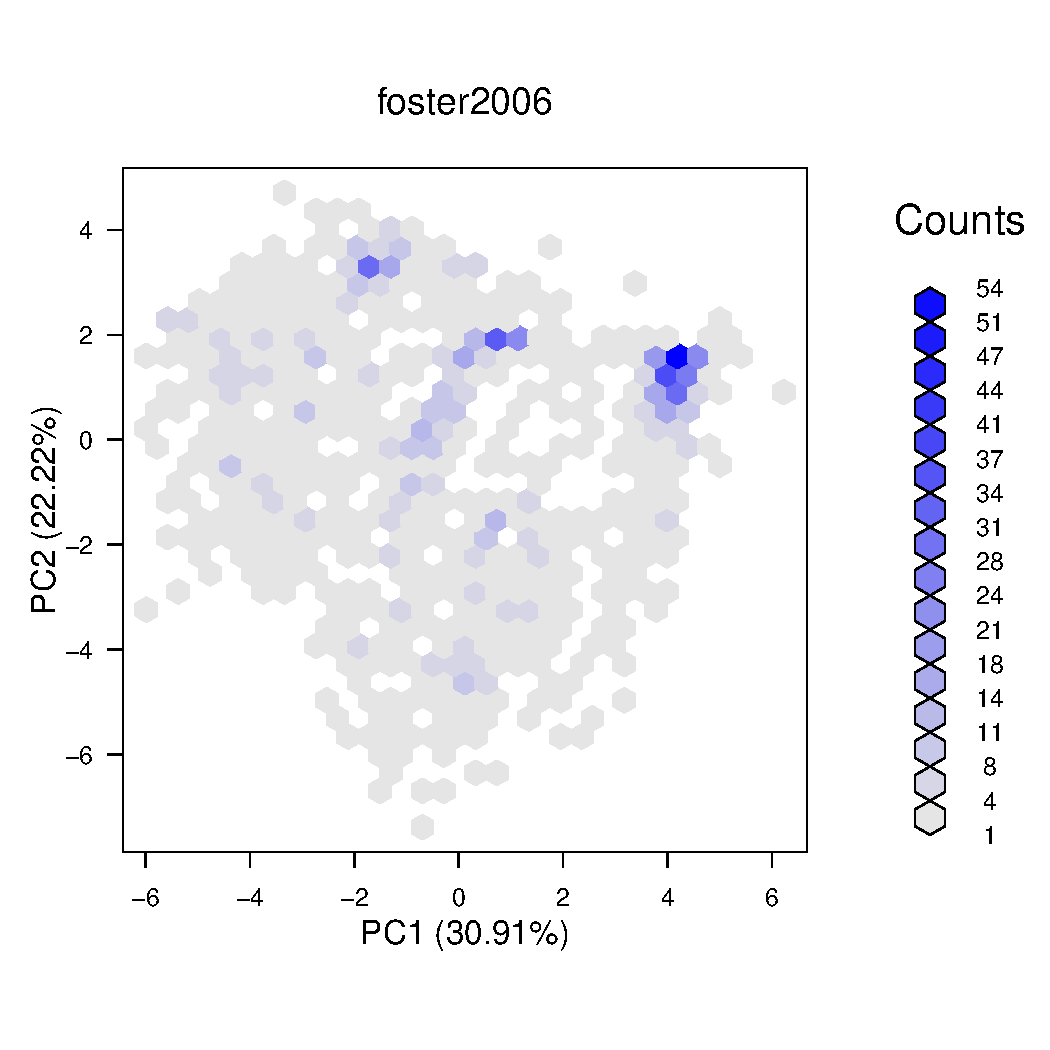
\includegraphics[width = 0.32\textwidth]{./figure/fighexpca-27.pdf}
  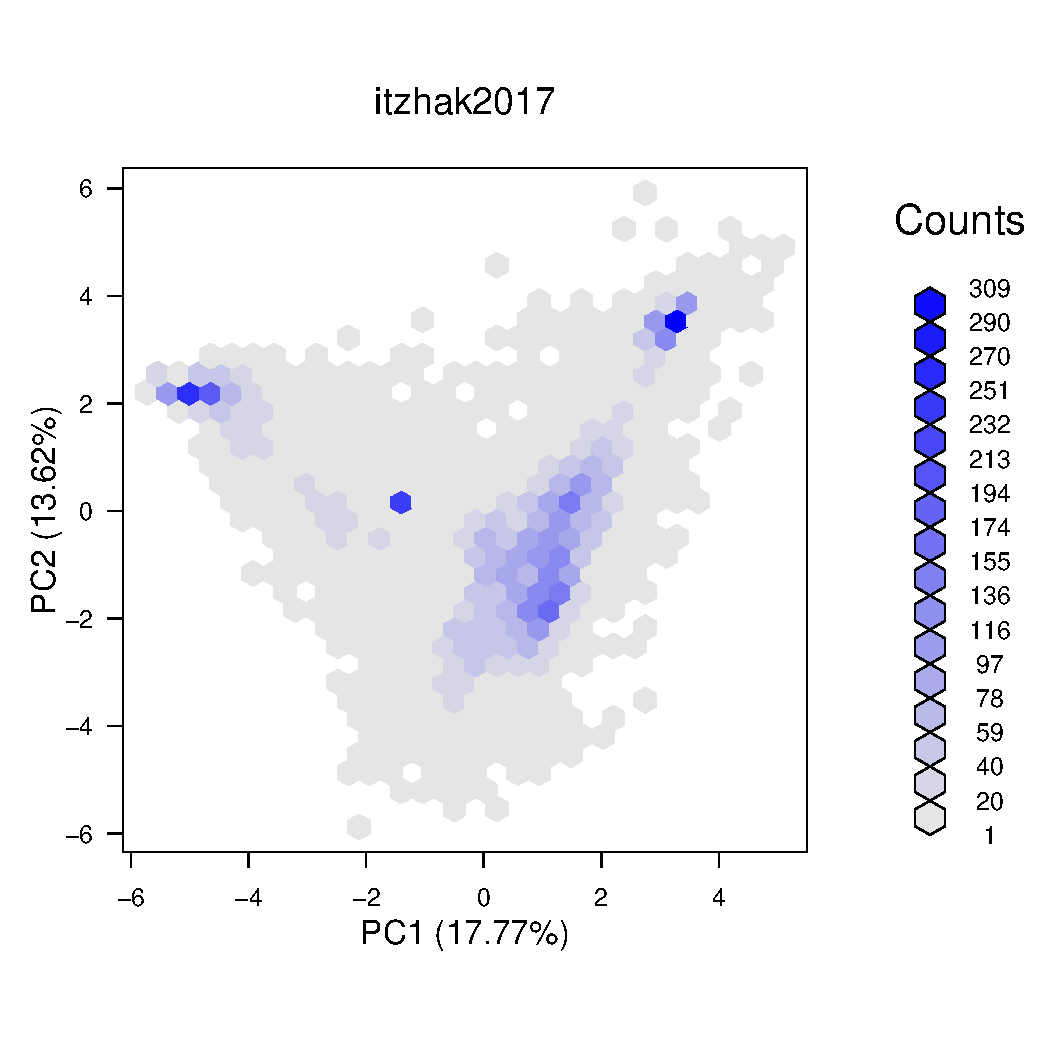
\includegraphics[width = 0.32\textwidth]{./figure/fighexpca-28.pdf}
  \caption{Density PCA plots for the 29 experiments
    used in this study. PC 1 and 2 were used except for
    \textit{itzhak2016stcSILAC}, where PC 1 and 3 were used to conform
    to the original authors figures. The experiments are ordered
    according to the median average between cluster distance (see
    figure~\ref{fig:qsep}). Figures have been generated using the
    \texttt{plot2D} function from the \Biocpkg{pRoloc} package.}
  \ContinuedFloat
  \label{fig:denspca}
\end{figure}


\begin{figure}[htb]
\centering
  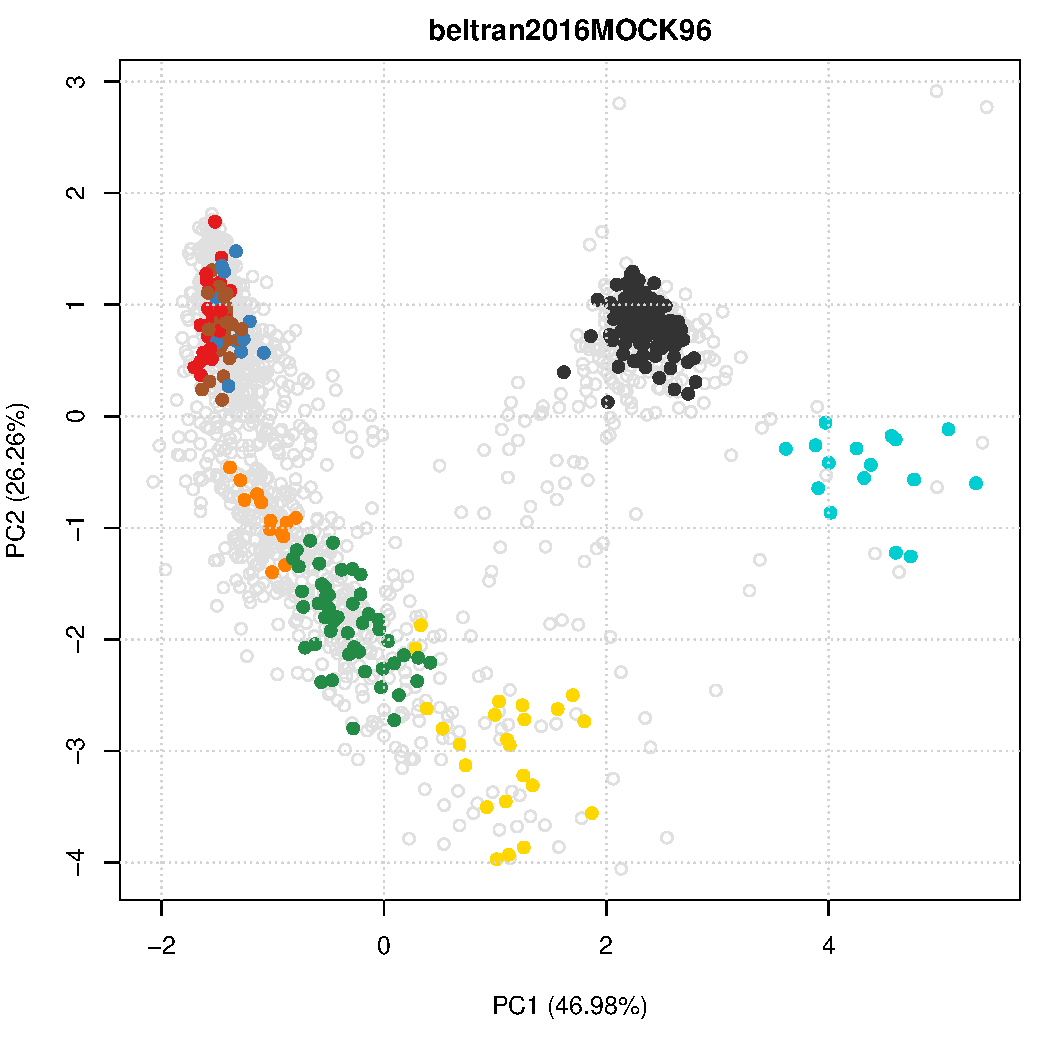
\includegraphics[width = 0.32\textwidth]{./figure/figpca-1.pdf}
  \includegraphics[width = 0.32\textwidth]{./figure/figpca-2.pdf}
  \includegraphics[width = 0.32\textwidth]{./figure/figpca-3.pdf}
  \includegraphics[width = 0.32\textwidth]{./figure/figpca-4.pdf}
  \includegraphics[width = 0.32\textwidth]{./figure/figpca-5.pdf}
  \includegraphics[width = 0.32\textwidth]{./figure/figpca-6.pdf}
  \includegraphics[width = 0.32\textwidth]{./figure/figpca-7.pdf}
  \includegraphics[width = 0.32\textwidth]{./figure/figpca-8.pdf}
  \includegraphics[width = 0.32\textwidth]{./figure/figpca-9.pdf}
  \includegraphics[width = 0.32\textwidth]{./figure/figpca-10.pdf}
  \includegraphics[width = 0.32\textwidth]{./figure/figpca-11.pdf}
  \includegraphics[width = 0.32\textwidth]{./figure/figpca-12.pdf}
\end{figure}
\begin{figure}[htb]\ContinuedFloat
  \includegraphics[width = 0.32\textwidth]{./figure/figpca-13.pdf}
  \includegraphics[width = 0.32\textwidth]{./figure/figpca-14.pdf}
  \includegraphics[width = 0.32\textwidth]{./figure/figpca-15.pdf}
  \includegraphics[width = 0.32\textwidth]{./figure/figpca-16.pdf}
  \includegraphics[width = 0.32\textwidth]{./figure/figpca-17.pdf}
  \includegraphics[width = 0.32\textwidth]{./figure/figpca-18.pdf}
  \includegraphics[width = 0.32\textwidth]{./figure/figpca-19.pdf}
  \includegraphics[width = 0.32\textwidth]{./figure/figpca-20.pdf}
  \includegraphics[width = 0.32\textwidth]{./figure/figpca-21.pdf}
  \includegraphics[width = 0.32\textwidth]{./figure/figpca-22.pdf}
  \includegraphics[width = 0.32\textwidth]{./figure/figpca-23.pdf}
  \includegraphics[width = 0.32\textwidth]{./figure/figpca-24.pdf}
\end{figure}
\begin{figure}[htb]
  \includegraphics[width = 0.32\textwidth]{./figure/figpca-25.pdf}
  \includegraphics[width = 0.32\textwidth]{./figure/figpca-26.pdf}
  \includegraphics[width = 0.32\textwidth]{./figure/figpca-27.pdf}
  \includegraphics[width = 0.32\textwidth]{./figure/figpca-28.pdf}
  \caption{PCA plots for the 29 experiments used in
    this study. PC 1 and 2 were used except for
    \textit{itzhak2016stcSILAC}, where PC 1 and 3 were used to conform
    to the original authors figures. The experiments are ordered
    according to the median average between cluster distance (see
    figure~\ref{fig:qsep}). The percentage of variance explained along
    the 2 PCs on the plots can be found in
    table~\ref{tab:pdtab}. Figures have been generated using the
    \texttt{plot2D} function from the \Biocpkg{pRoloc} package.}
  \ContinuedFloat
  \label{fig:pca}
\end{figure}

\begin{figure}[htb]
  \centering
  \includegraphics[width = 0.32\textwidth]{./figure/allqseps-1.pdf}
  \includegraphics[width = 0.32\textwidth]{./figure/allqseps-2.pdf}
  \includegraphics[width = 0.32\textwidth]{./figure/allqseps-3.pdf}
  \includegraphics[width = 0.32\textwidth]{./figure/allqseps-4.pdf}
  \includegraphics[width = 0.32\textwidth]{./figure/allqseps-5.pdf}
  \includegraphics[width = 0.32\textwidth]{./figure/allqseps-6.pdf}
  \includegraphics[width = 0.32\textwidth]{./figure/allqseps-7.pdf}
  \includegraphics[width = 0.32\textwidth]{./figure/allqseps-8.pdf}
  \includegraphics[width = 0.32\textwidth]{./figure/allqseps-9.pdf}
  \includegraphics[width = 0.32\textwidth]{./figure/allqseps-10.pdf}
  \includegraphics[width = 0.32\textwidth]{./figure/allqseps-11.pdf}
  \includegraphics[width = 0.32\textwidth]{./figure/allqseps-12.pdf}
\end{figure}
\begin{figure}[htb]\ContinuedFloat
  \includegraphics[width = 0.32\textwidth]{./figure/allqseps-13.pdf}
  \includegraphics[width = 0.32\textwidth]{./figure/allqseps-14.pdf}
  \includegraphics[width = 0.32\textwidth]{./figure/allqseps-15.pdf}
  \includegraphics[width = 0.32\textwidth]{./figure/allqseps-16.pdf}
  \includegraphics[width = 0.32\textwidth]{./figure/allqseps-17.pdf}
  \includegraphics[width = 0.32\textwidth]{./figure/allqseps-18.pdf}
  \includegraphics[width = 0.32\textwidth]{./figure/allqseps-19.pdf}
  \includegraphics[width = 0.32\textwidth]{./figure/allqseps-20.pdf}
  \includegraphics[width = 0.32\textwidth]{./figure/allqseps-21.pdf}
  \includegraphics[width = 0.32\textwidth]{./figure/allqseps-22.pdf}
  \includegraphics[width = 0.32\textwidth]{./figure/allqseps-23.pdf}
  \includegraphics[width = 0.32\textwidth]{./figure/allqseps-24.pdf}
\end{figure}
\begin{figure}[htb]
  \includegraphics[width = 0.32\textwidth]{./figure/allqseps-25.pdf}
  \includegraphics[width = 0.32\textwidth]{./figure/allqseps-26.pdf}
  \includegraphics[width = 0.32\textwidth]{./figure/allqseps-27.pdf}
  \includegraphics[width = 0.32\textwidth]{./figure/allqseps-28.pdf}
  \caption{Quantitative separation boxplot for the 29
    experiments used in this study. The experiments are ordered
    according to the median average between cluster distance (see
    figure~\ref{fig:qsep}). }
  \ContinuedFloat
  \label{fig:allqseps}
\end{figure}

\begin{figure}[htb]
  \centering
  \includegraphics[width = 0.32\textwidth]{./figure/allhmaps-1.pdf}
  \includegraphics[width = 0.32\textwidth]{./figure/allhmaps-2.pdf}
  \includegraphics[width = 0.32\textwidth]{./figure/allhmaps-3.pdf}
  \includegraphics[width = 0.32\textwidth]{./figure/allhmaps-4.pdf}
  \includegraphics[width = 0.32\textwidth]{./figure/allhmaps-5.pdf}
  \includegraphics[width = 0.32\textwidth]{./figure/allhmaps-6.pdf}
  \includegraphics[width = 0.32\textwidth]{./figure/allhmaps-7.pdf}
  \includegraphics[width = 0.32\textwidth]{./figure/allhmaps-8.pdf}
  \includegraphics[width = 0.32\textwidth]{./figure/allhmaps-9.pdf}
  \includegraphics[width = 0.32\textwidth]{./figure/allhmaps-10.pdf}
  \includegraphics[width = 0.32\textwidth]{./figure/allhmaps-11.pdf}
  \includegraphics[width = 0.32\textwidth]{./figure/allhmaps-12.pdf}
\end{figure}
\begin{figure}[htb]\ContinuedFloat
  \includegraphics[width = 0.32\textwidth]{./figure/allhmaps-13.pdf}
  \includegraphics[width = 0.32\textwidth]{./figure/allhmaps-14.pdf}
  \includegraphics[width = 0.32\textwidth]{./figure/allhmaps-15.pdf}
  \includegraphics[width = 0.32\textwidth]{./figure/allhmaps-16.pdf}
  \includegraphics[width = 0.32\textwidth]{./figure/allhmaps-17.pdf}
  \includegraphics[width = 0.32\textwidth]{./figure/allhmaps-18.pdf}
  \includegraphics[width = 0.32\textwidth]{./figure/allhmaps-19.pdf}
  \includegraphics[width = 0.32\textwidth]{./figure/allhmaps-20.pdf}
  \includegraphics[width = 0.32\textwidth]{./figure/allhmaps-21.pdf}
  \includegraphics[width = 0.32\textwidth]{./figure/allhmaps-22.pdf}
  \includegraphics[width = 0.32\textwidth]{./figure/allhmaps-23.pdf}
  \includegraphics[width = 0.32\textwidth]{./figure/allhmaps-24.pdf}
\end{figure}
\begin{figure}[htb]
  \includegraphics[width = 0.32\textwidth]{./figure/allhmaps-25.pdf}
  \includegraphics[width = 0.32\textwidth]{./figure/allhmaps-26.pdf}
  \includegraphics[width = 0.32\textwidth]{./figure/allhmaps-27.pdf}
  \includegraphics[width = 0.32\textwidth]{./figure/allhmaps-28.pdf}
  \caption{Quantitative separation heatmaps for the 29
    experiments used in this study. The experiments are ordered
    according to the median average between cluster distance (see
    figure~\ref{fig:qsep}). }
  \ContinuedFloat
  \label{fig:allhmaps}
\end{figure}

\clearpage

\section{Session information}

The software and versions used to produce this document are summarised
below. The source of this document enabling to reproduce all results
and figures is available in the source of this document in the public
manuscript repository~\cite{qseprepo} available at
\url{https://github.com/lgatto/QSep-manuscript/}.

\begin{itemize}\raggedright
  \item R Under development (unstable) (2018-04-02 r74505), \verb|x86_64-pc-linux-gnu|
  \item Running under: \verb|Ubuntu 14.04.5 LTS|
  \item Matrix products: default
  \item BLAS: \verb|/usr/lib/atlas-base/atlas/libblas.so.3.0|
  \item LAPACK: \verb|/usr/lib/lapack/liblapack.so.3.0|
  \item Base packages: base, datasets, graphics, grDevices,
    methods, parallel, stats, stats4, utils
  \item Other packages: annotate~1.58.0, AnnotationDbi~1.42.1,
    Biobase~2.40.0, BiocGenerics~0.26.0, BiocParallel~1.14.2,
    cluster~2.0.7-1, ggplot2~3.0.0, ggrepel~0.8.0, hexbin~1.27.2,
    IRanges~2.14.10, MLInterfaces~1.60.1, MSnbase~2.7.3,
    mzR~2.15.2, pRoloc~1.21.7, pRolocdata~1.18.0,
    ProtGenerics~1.12.0, Rcpp~0.12.18, S4Vectors~0.18.3,
    XML~3.98-1.12, xtable~1.8-2
  \item Loaded via a namespace (and not attached): abind~1.4-5,
    affy~1.58.0, affyio~1.50.0, assertthat~0.2.0, backports~1.1.2,
    base64enc~0.1-3, bindr~0.1.1, bindrcpp~0.2.2,
    BiocInstaller~1.30.0, biomaRt~2.36.1, bit~1.1-14, bit64~0.9-7,
    bitops~1.0-6, blob~1.1.1, broom~0.5.0, caret~6.0-80,
    class~7.3-14, coda~0.19-1, codetools~0.2-15, colorspace~1.3-2,
    compiler~3.6.0, crayon~1.3.4, crosstalk~1.0.0, CVST~0.2-2,
    DBI~1.0.0, ddalpha~1.3.4, dendextend~1.8.0, DEoptimR~1.0-8,
    digest~0.6.15, dimRed~0.1.0, diptest~0.75-7,
    doParallel~1.0.11, dplyr~0.7.6, DRR~0.0.3, e1071~1.6-8,
    evaluate~0.11, flexmix~2.3-14, FNN~1.1, foreach~1.4.4,
    fpc~2.1-11.1, gbm~2.1.3, gdata~2.18.0, genefilter~1.62.0,
    geometry~0.3-6, ggvis~0.4.3, glue~1.3.0, gower~0.1.2,
    grid~3.6.0, gridExtra~2.3, gtable~0.2.0, gtools~3.8.1,
    highr~0.7, hms~0.4.2, htmltools~0.3.6, htmlwidgets~1.2,
    httpuv~1.4.5, httr~1.3.1, hwriter~1.3.2, igraph~1.2.1,
    impute~1.54.0, ipred~0.9-6, iterators~1.0.10, kernlab~0.9-26,
    knitr~1.20, labeling~0.3, LaplacesDemon~16.1.1, later~0.7.3,
    lattice~0.20-35, lava~1.6.2, lazyeval~0.2.1, limma~3.36.2,
    lpSolve~5.6.13, lubridate~1.7.4, magic~1.5-8, magrittr~1.5,
    MALDIquant~1.18, MASS~7.3-50, Matrix~1.2-14, mclust~5.4.1,
    memoise~1.1.0, mime~0.5, mixtools~1.1.0, mlbench~2.1-1,
    ModelMetrics~1.1.0, modeltools~0.2-22, munsell~0.5.0,
    mvtnorm~1.0-8, mzID~1.18.0, nlme~3.1-137, nnet~7.3-12,
    pcaMethods~1.72.0, pillar~1.3.0, pkgconfig~2.0.1, pls~2.6-0,
    plyr~1.8.4, prabclus~2.2-6, preprocessCore~1.42.0,
    prettyunits~1.0.2, prodlim~2018.04.18, progress~1.2.0,
    promises~1.0.1, proxy~0.4-22, purrr~0.2.5, R6~2.2.2,
    randomForest~4.6-14, RColorBrewer~1.1-2, RcppRoll~0.3.0,
    RCurl~1.95-4.11, rda~1.0.2-2.1, recipes~0.1.3, reshape2~1.4.3,
    rlang~0.2.1, robustbase~0.93-1.1, rpart~4.1-13, RSQLite~2.1.1,
    sampling~2.8, scales~0.5.0, segmented~0.5-3.0, sfsmisc~1.1-2,
    shiny~1.1.0, splines~3.6.0, stringi~1.2.4, stringr~1.3.1,
    survival~2.42-4, threejs~0.3.1, tibble~1.4.2, tidyr~0.8.1,
    tidyselect~0.2.4, timeDate~3043.102, tools~3.6.0,
    trimcluster~0.1-2.1, viridis~0.5.1, viridisLite~0.3.0,
    vsn~3.48.1, whisker~0.3-2, withr~2.1.2, zlibbioc~1.26.0
\end{itemize}


\end{appendices}

\bibliographystyle{plainnat}
\bibliography{qsep}

\end{document}
